\documentclass[]{book}
\usepackage{lmodern}
\usepackage{amssymb,amsmath}
\usepackage{ifxetex,ifluatex}
\usepackage{fixltx2e} % provides \textsubscript
\ifnum 0\ifxetex 1\fi\ifluatex 1\fi=0 % if pdftex
  \usepackage[T1]{fontenc}
  \usepackage[utf8]{inputenc}
\else % if luatex or xelatex
  \ifxetex
    \usepackage{mathspec}
  \else
    \usepackage{fontspec}
  \fi
  \defaultfontfeatures{Ligatures=TeX,Scale=MatchLowercase}
\fi
% use upquote if available, for straight quotes in verbatim environments
\IfFileExists{upquote.sty}{\usepackage{upquote}}{}
% use microtype if available
\IfFileExists{microtype.sty}{%
\usepackage{microtype}
\UseMicrotypeSet[protrusion]{basicmath} % disable protrusion for tt fonts
}{}
\usepackage[margin=1in]{geometry}
\usepackage{hyperref}
\hypersetup{unicode=true,
            pdftitle={Notebook},
            pdfauthor={Aji John},
            pdfborder={0 0 0},
            breaklinks=true}
\urlstyle{same}  % don't use monospace font for urls
\usepackage{natbib}
\bibliographystyle{apalike}
\usepackage{color}
\usepackage{fancyvrb}
\newcommand{\VerbBar}{|}
\newcommand{\VERB}{\Verb[commandchars=\\\{\}]}
\DefineVerbatimEnvironment{Highlighting}{Verbatim}{commandchars=\\\{\}}
% Add ',fontsize=\small' for more characters per line
\usepackage{framed}
\definecolor{shadecolor}{RGB}{248,248,248}
\newenvironment{Shaded}{\begin{snugshade}}{\end{snugshade}}
\newcommand{\KeywordTok}[1]{\textcolor[rgb]{0.13,0.29,0.53}{\textbf{#1}}}
\newcommand{\DataTypeTok}[1]{\textcolor[rgb]{0.13,0.29,0.53}{#1}}
\newcommand{\DecValTok}[1]{\textcolor[rgb]{0.00,0.00,0.81}{#1}}
\newcommand{\BaseNTok}[1]{\textcolor[rgb]{0.00,0.00,0.81}{#1}}
\newcommand{\FloatTok}[1]{\textcolor[rgb]{0.00,0.00,0.81}{#1}}
\newcommand{\ConstantTok}[1]{\textcolor[rgb]{0.00,0.00,0.00}{#1}}
\newcommand{\CharTok}[1]{\textcolor[rgb]{0.31,0.60,0.02}{#1}}
\newcommand{\SpecialCharTok}[1]{\textcolor[rgb]{0.00,0.00,0.00}{#1}}
\newcommand{\StringTok}[1]{\textcolor[rgb]{0.31,0.60,0.02}{#1}}
\newcommand{\VerbatimStringTok}[1]{\textcolor[rgb]{0.31,0.60,0.02}{#1}}
\newcommand{\SpecialStringTok}[1]{\textcolor[rgb]{0.31,0.60,0.02}{#1}}
\newcommand{\ImportTok}[1]{#1}
\newcommand{\CommentTok}[1]{\textcolor[rgb]{0.56,0.35,0.01}{\textit{#1}}}
\newcommand{\DocumentationTok}[1]{\textcolor[rgb]{0.56,0.35,0.01}{\textbf{\textit{#1}}}}
\newcommand{\AnnotationTok}[1]{\textcolor[rgb]{0.56,0.35,0.01}{\textbf{\textit{#1}}}}
\newcommand{\CommentVarTok}[1]{\textcolor[rgb]{0.56,0.35,0.01}{\textbf{\textit{#1}}}}
\newcommand{\OtherTok}[1]{\textcolor[rgb]{0.56,0.35,0.01}{#1}}
\newcommand{\FunctionTok}[1]{\textcolor[rgb]{0.00,0.00,0.00}{#1}}
\newcommand{\VariableTok}[1]{\textcolor[rgb]{0.00,0.00,0.00}{#1}}
\newcommand{\ControlFlowTok}[1]{\textcolor[rgb]{0.13,0.29,0.53}{\textbf{#1}}}
\newcommand{\OperatorTok}[1]{\textcolor[rgb]{0.81,0.36,0.00}{\textbf{#1}}}
\newcommand{\BuiltInTok}[1]{#1}
\newcommand{\ExtensionTok}[1]{#1}
\newcommand{\PreprocessorTok}[1]{\textcolor[rgb]{0.56,0.35,0.01}{\textit{#1}}}
\newcommand{\AttributeTok}[1]{\textcolor[rgb]{0.77,0.63,0.00}{#1}}
\newcommand{\RegionMarkerTok}[1]{#1}
\newcommand{\InformationTok}[1]{\textcolor[rgb]{0.56,0.35,0.01}{\textbf{\textit{#1}}}}
\newcommand{\WarningTok}[1]{\textcolor[rgb]{0.56,0.35,0.01}{\textbf{\textit{#1}}}}
\newcommand{\AlertTok}[1]{\textcolor[rgb]{0.94,0.16,0.16}{#1}}
\newcommand{\ErrorTok}[1]{\textcolor[rgb]{0.64,0.00,0.00}{\textbf{#1}}}
\newcommand{\NormalTok}[1]{#1}
\usepackage{longtable,booktabs}
\usepackage{graphicx,grffile}
\makeatletter
\def\maxwidth{\ifdim\Gin@nat@width>\linewidth\linewidth\else\Gin@nat@width\fi}
\def\maxheight{\ifdim\Gin@nat@height>\textheight\textheight\else\Gin@nat@height\fi}
\makeatother
% Scale images if necessary, so that they will not overflow the page
% margins by default, and it is still possible to overwrite the defaults
% using explicit options in \includegraphics[width, height, ...]{}
\setkeys{Gin}{width=\maxwidth,height=\maxheight,keepaspectratio}
\IfFileExists{parskip.sty}{%
\usepackage{parskip}
}{% else
\setlength{\parindent}{0pt}
\setlength{\parskip}{6pt plus 2pt minus 1pt}
}
\setlength{\emergencystretch}{3em}  % prevent overfull lines
\providecommand{\tightlist}{%
  \setlength{\itemsep}{0pt}\setlength{\parskip}{0pt}}
\setcounter{secnumdepth}{5}
% Redefines (sub)paragraphs to behave more like sections
\ifx\paragraph\undefined\else
\let\oldparagraph\paragraph
\renewcommand{\paragraph}[1]{\oldparagraph{#1}\mbox{}}
\fi
\ifx\subparagraph\undefined\else
\let\oldsubparagraph\subparagraph
\renewcommand{\subparagraph}[1]{\oldsubparagraph{#1}\mbox{}}
\fi

%%% Use protect on footnotes to avoid problems with footnotes in titles
\let\rmarkdownfootnote\footnote%
\def\footnote{\protect\rmarkdownfootnote}

%%% Change title format to be more compact
\usepackage{titling}

% Create subtitle command for use in maketitle
\newcommand{\subtitle}[1]{
  \posttitle{
    \begin{center}\large#1\end{center}
    }
}

\setlength{\droptitle}{-2em}
  \title{Notebook}
  \pretitle{\vspace{\droptitle}\centering\huge}
  \posttitle{\par}
  \author{Aji John}
  \preauthor{\centering\large\emph}
  \postauthor{\par}
  \predate{\centering\large\emph}
  \postdate{\par}
  \date{2018-07-26}

\usepackage{booktabs}
\usepackage{amsthm}
\makeatletter
\def\thm@space@setup{%
  \thm@preskip=8pt plus 2pt minus 4pt
  \thm@postskip=\thm@preskip
}
\makeatother

\usepackage{amsthm}
\newtheorem{theorem}{Theorem}[chapter]
\newtheorem{lemma}{Lemma}[chapter]
\theoremstyle{definition}
\newtheorem{definition}{Definition}[chapter]
\newtheorem{corollary}{Corollary}[chapter]
\newtheorem{proposition}{Proposition}[chapter]
\theoremstyle{definition}
\newtheorem{example}{Example}[chapter]
\theoremstyle{definition}
\newtheorem{exercise}{Exercise}[chapter]
\theoremstyle{remark}
\newtheorem*{remark}{Remark}
\newtheorem*{solution}{Solution}
\begin{document}
\maketitle

{
\setcounter{tocdepth}{1}
\tableofcontents
}
\chapter{Preamble}\label{preamble}

I am a PhD student in Biology at University of Washington. I'm intersted
in boundary layer climate, and the effects of microclimates(think of
climate right above ground) on plants and animals. I like to develop
\emph{computational tools} in \textbf{R and Python}. I embrace openness
in research and believe in sharing knowledge.

Below are the packages developed in \emph{\textbf{R}} that could be used
in any field.

\begin{Shaded}
\begin{Highlighting}[]
\CommentTok{# TrenchR - Energy balance functions}
\CommentTok{# devtools::install_github("trenchproject/TrenchR")}
\CommentTok{# TrenchR - UI to extract microclimate data}
\CommentTok{# devtools::install_github("trenchproject/ebm")}
\CommentTok{# TrenchR - Backend processor for UI (Uses Amazon Mail API)}
\CommentTok{# devtools::install_github("trenchproject/tecor-monitor")}
\end{Highlighting}
\end{Shaded}

Few sites where my research can be visualized. Extract microclimate data
at \url{http://microclim.org/}.

\section{Areas of interest}\label{areas-of-interest}

\section{Published papers}\label{published-papers}

Ausmees, Kristiina, Aji John, Salman Z. Toor, Andreas Hellander, and
Carl Nettelblad. ``BAMSI: a multi-cloud service for scalable distributed
filtering of massive genome data.'' BMC bioinformatics 19, no. 1 (2018):
240.

Ausmees, Kristiina, and Pushpam Aji John. ``Analysis of Chromosome 20-A
Study.'' arXiv preprint arXiv:1607.00276 (2016).

John, Pushpam Aji, et al. ``868 MHz Wireless Sensor Network-A Study.''
arXiv preprint arXiv:1609.00475 (2016).

\section{Un-Published papers}\label{un-published-papers}

\chapter{Introduction}\label{intro}

You can label chapter and section titles using \texttt{\{\#label\}}
after them, e.g., we can reference Chapter \ref{intro}. If you do not
manually label them, there will be automatic labels anyway, e.g.,
Chapter \ref{methods}.

Figures and tables with captions will be placed in \texttt{figure} and
\texttt{table} environments, respectively.

Reference a figure by its code chunk label with the \texttt{fig:}
prefix, e.g., see Figure \ref{fig:nice-fig}. Similarly, you can
reference tables generated from \texttt{knitr::kable()}, e.g., see Table
\ref{tab:nice-tab}.

You can write citations, too. For example, we are using the
\textbf{bookdown} package \citep{R-bookdown} in this sample book, which
was built on top of R Markdown and \textbf{knitr} \citep{aj2018}.

\chapter{Background}\label{background}

This section deals with what I had to learn or I learnt from the courses
I took. You can label chapter and section titles using
\texttt{\{\#label\}} after them, e.g., we can reference Chapter
\ref{intro}. If you do not manually label them, there will be automatic
labels anyway, e.g., Chapter \ref{methods}.

Figures and tables with captions will be placed in \texttt{figure} and
\texttt{table} environments, respectively.

\begin{Shaded}
\begin{Highlighting}[]
\KeywordTok{par}\NormalTok{(}\DataTypeTok{mar =} \KeywordTok{c}\NormalTok{(}\DecValTok{4}\NormalTok{, }\DecValTok{4}\NormalTok{, .}\DecValTok{1}\NormalTok{, .}\DecValTok{1}\NormalTok{))}
\KeywordTok{plot}\NormalTok{(pressure, }\DataTypeTok{type =} \StringTok{'b'}\NormalTok{, }\DataTypeTok{pch =} \DecValTok{19}\NormalTok{)}
\end{Highlighting}
\end{Shaded}

\begin{figure}

{\centering 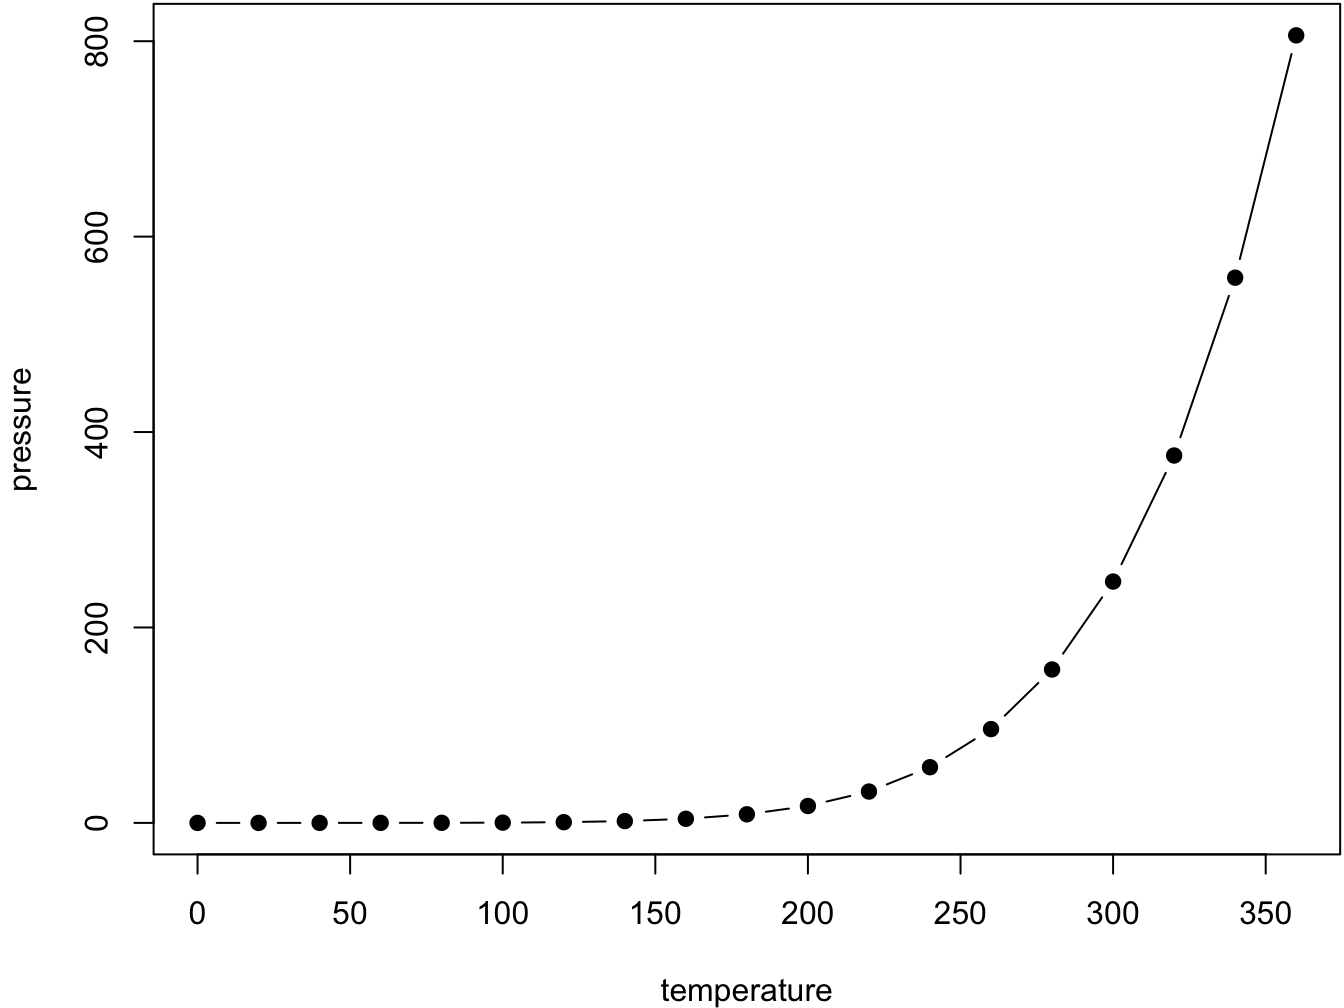
\includegraphics[width=0.8\linewidth]{Research_book_files/figure-latex/nice-fig-1} 

}

\caption{Here is a nice figure!}\label{fig:nice-fig}
\end{figure}

Reference a figure by its code chunk label with the \texttt{fig:}
prefix, e.g., see Figure \ref{fig:nice-fig}. Similarly, you can
reference tables generated from \texttt{knitr::kable()}, e.g., see Table
\ref{tab:nice-tab}.

\begin{Shaded}
\begin{Highlighting}[]
\NormalTok{knitr}\OperatorTok{::}\KeywordTok{kable}\NormalTok{(}
  \KeywordTok{head}\NormalTok{(iris, }\DecValTok{20}\NormalTok{), }\DataTypeTok{caption =} \StringTok{'Here is a nice table!'}\NormalTok{,}
  \DataTypeTok{booktabs =} \OtherTok{TRUE}
\NormalTok{)}
\end{Highlighting}
\end{Shaded}

\begin{table}

\caption{\label{tab:nice-tab}Here is a nice table!}
\centering
\begin{tabular}[t]{rrrrl}
\toprule
Sepal.Length & Sepal.Width & Petal.Length & Petal.Width & Species\\
\midrule
5.1 & 3.5 & 1.4 & 0.2 & setosa\\
4.9 & 3.0 & 1.4 & 0.2 & setosa\\
4.7 & 3.2 & 1.3 & 0.2 & setosa\\
4.6 & 3.1 & 1.5 & 0.2 & setosa\\
5.0 & 3.6 & 1.4 & 0.2 & setosa\\
\addlinespace
5.4 & 3.9 & 1.7 & 0.4 & setosa\\
4.6 & 3.4 & 1.4 & 0.3 & setosa\\
5.0 & 3.4 & 1.5 & 0.2 & setosa\\
4.4 & 2.9 & 1.4 & 0.2 & setosa\\
4.9 & 3.1 & 1.5 & 0.1 & setosa\\
\addlinespace
5.4 & 3.7 & 1.5 & 0.2 & setosa\\
4.8 & 3.4 & 1.6 & 0.2 & setosa\\
4.8 & 3.0 & 1.4 & 0.1 & setosa\\
4.3 & 3.0 & 1.1 & 0.1 & setosa\\
5.8 & 4.0 & 1.2 & 0.2 & setosa\\
\addlinespace
5.7 & 4.4 & 1.5 & 0.4 & setosa\\
5.4 & 3.9 & 1.3 & 0.4 & setosa\\
5.1 & 3.5 & 1.4 & 0.3 & setosa\\
5.7 & 3.8 & 1.7 & 0.3 & setosa\\
5.1 & 3.8 & 1.5 & 0.3 & setosa\\
\bottomrule
\end{tabular}
\end{table}

You can write citations, too. For example, we are using the
\textbf{bookdown} package \citep{R-bookdown} in this sample book, which
was built on top of R Markdown and \textbf{knitr} \citep{aj2018}.

\section{Algaebra}\label{algaebra}

\section{Statistics}\label{statistics}

\chapter{Literature}\label{literature}

Here is a review of existing methods.

\chapter{Methods}\label{methods}

We describe our methods in this chapter.

\chapter{Applications}\label{applications}

Some \emph{significant} applications are demonstrated in this chapter.

\section{Example one}\label{example-one}

\section{Example two}\label{example-two}

\chapter{Final Words}\label{final-words}

We have finished a nice book.

\chapter{Journal}\label{journal}

Daily \emph{lab notes}

\begin{Shaded}
\begin{Highlighting}[]
\KeywordTok{library}\NormalTok{(ggplot2)}
\KeywordTok{library}\NormalTok{(tidyverse)}
\KeywordTok{library}\NormalTok{(lubridate)}
\end{Highlighting}
\end{Shaded}

\section{4-12-2018}\label{section}

\subsection{ekoseminar}\label{ekoseminar}

Urban ecosystems are undergoing evolution at a much faster pace than one
would imagine. Thinking about mutation which introduce allele frequency
key to heritable diversity ?

\subsection{meeting with jhrl}\label{meeting-with-jhrl}

Certain species do flower early - confirmed by JHRL. The poster we
presented does make sense.

\subsection{ekoclimate}\label{ekoclimate}

The energy budget of the area increases if the type of the cover
changes, i.e if it changes from deciduous forest to crop/grassland then
the net Long Wave radiation(flux?) increases. Long wave is the one that
is reflected, so the area with a grass will absorb more heat through the
day , and emilt radiation during the night? (More cooling ?). So, should
we see more diurnal variation in crop/grasslands than forests ?. How
should one charaterize the total energy flux on grasslands vs forests?

Shortware is the incoming radiation - i.e having a shorter wavelength,
and when is reflected, it becomes long wave radiation. The longwave
radiation emitted out is calculated by multipying Stephan Boltzman
constant multiplied by epsilion(emissivity) and
Temperature\^{}4(Temperature of the object).

\subsection{trenchR}\label{trenchr}

Thermal conductance wrt to animals define the amount of heat which can
escape out of animals. It depends on the difference between the animal
and the outside temperature and you multipy by the thickness(lambda) and
a proportion of the surface area(true area exposed to solar radiation).

Surace area to calculate the exposure is related to the exposed area -
tricky as animals come in all shapes, mostly cylindrical with a sphere
head if land based.

\section{4-13-2018}\label{section-1}

\section{4-20-2008}\label{section-2}

Heat transfer coefficient for Lizards. It is linear with windspeeed, and
slope changes when the lizard is parallel or transverse

\section{4-23-2008}\label{section-3}

Get diurnal variation across 5 sites at Mt Rainier

\begin{Shaded}
\begin{Highlighting}[]
\CommentTok{#Load a file}
\NormalTok{Paradise_}\DecValTok{2017}\NormalTok{<-}\StringTok{ }\KeywordTok{read.csv}\NormalTok{(}\StringTok{'./data/ParadiseWind_5380_feet_2017.csv'}\NormalTok{)}
\NormalTok{CampMuir_}\DecValTok{2017}\NormalTok{<-}\StringTok{ }\KeywordTok{read.csv}\NormalTok{(}\StringTok{'./data/CampMuir_10110_feet_2017.csv'}\NormalTok{)}
\NormalTok{Sunriseupper_}\DecValTok{2017}\NormalTok{<-}\StringTok{ }\KeywordTok{read.csv}\NormalTok{(}\StringTok{'./data/SunriseUpper_6880_feet_2017.csv'}\NormalTok{)}

\NormalTok{Paradise_}\DecValTok{2017}\OperatorTok{$}\NormalTok{date <-}\StringTok{ }\KeywordTok{as.Date}\NormalTok{(Paradise_}\DecValTok{2017}\OperatorTok{$}\NormalTok{Date.Time..PST., }\StringTok{"%Y-%m-%d"}\NormalTok{)}
\NormalTok{Paradise_}\DecValTok{2017}\OperatorTok{$}\NormalTok{hr <-}\KeywordTok{strftime}\NormalTok{(Paradise_}\DecValTok{2017}\OperatorTok{$}\NormalTok{Date.Time..PST.,}\StringTok{'%H'}\NormalTok{)}
\NormalTok{Paradise_}\DecValTok{2017}\OperatorTok{$}\NormalTok{min <-}\KeywordTok{strftime}\NormalTok{(Paradise_}\DecValTok{2017}\OperatorTok{$}\NormalTok{Date.Time..PST.,}\StringTok{'%M'}\NormalTok{)}
\NormalTok{Paradise_}\DecValTok{2017}\OperatorTok{$}\NormalTok{month <-}\StringTok{ }\KeywordTok{strftime}\NormalTok{(Paradise_}\DecValTok{2017}\OperatorTok{$}\NormalTok{Date.Time..PST.,}\StringTok{'%m'}\NormalTok{)}
\NormalTok{CampMuir_}\DecValTok{2017}\OperatorTok{$}\NormalTok{date <-}\StringTok{ }\KeywordTok{as.Date}\NormalTok{(CampMuir_}\DecValTok{2017}\OperatorTok{$}\NormalTok{Date.Time..PST., }\StringTok{"%Y-%m-%d"}\NormalTok{)}
\NormalTok{CampMuir_}\DecValTok{2017}\OperatorTok{$}\NormalTok{hr <-}\KeywordTok{strftime}\NormalTok{(CampMuir_}\DecValTok{2017}\OperatorTok{$}\NormalTok{Date.Time..PST.,}\StringTok{'%H'}\NormalTok{)}
\NormalTok{CampMuir_}\DecValTok{2017}\OperatorTok{$}\NormalTok{min <-}\KeywordTok{strftime}\NormalTok{(CampMuir_}\DecValTok{2017}\OperatorTok{$}\NormalTok{Date.Time..PST.,}\StringTok{'%M'}\NormalTok{)}
\NormalTok{CampMuir_}\DecValTok{2017}\OperatorTok{$}\NormalTok{month <-}\KeywordTok{strftime}\NormalTok{(CampMuir_}\DecValTok{2017}\OperatorTok{$}\NormalTok{Date.Time..PST.,}\StringTok{'%m'}\NormalTok{)}
\NormalTok{Sunriseupper_}\DecValTok{2017}\OperatorTok{$}\NormalTok{date <-}\StringTok{ }\KeywordTok{as.Date}\NormalTok{(Sunriseupper_}\DecValTok{2017}\OperatorTok{$}\NormalTok{Date.Time..PST., }\StringTok{"%Y-%m-%d"}\NormalTok{)}
\NormalTok{Sunriseupper_}\DecValTok{2017}\OperatorTok{$}\NormalTok{hr <-}\KeywordTok{strftime}\NormalTok{(Sunriseupper_}\DecValTok{2017}\OperatorTok{$}\NormalTok{Date.Time..PST.,}\StringTok{'%H'}\NormalTok{)}
\NormalTok{Sunriseupper_}\DecValTok{2017}\OperatorTok{$}\NormalTok{min <-}\KeywordTok{strftime}\NormalTok{(Sunriseupper_}\DecValTok{2017}\OperatorTok{$}\NormalTok{Date.Time..PST.,}\StringTok{'%M'}\NormalTok{)}
\NormalTok{Sunriseupper_}\DecValTok{2017}\OperatorTok{$}\NormalTok{month <-}\StringTok{ }\KeywordTok{strftime}\NormalTok{(Sunriseupper_}\DecValTok{2017}\OperatorTok{$}\NormalTok{Date.Time..PST.,}\StringTok{'%m'}\NormalTok{)}


\KeywordTok{str}\NormalTok{(Paradise_}\DecValTok{2017}\NormalTok{)}
\end{Highlighting}
\end{Shaded}

\begin{verbatim}
## 'data.frame':    8760 obs. of  11 variables:
##  $ Date.Time..PST.         : Factor w/ 8760 levels "2017-01-01 00:00",..: 8760 8759 8758 8757 8756 8755 8754 8753 8752 8751 ...
##  $ Battery.Voltage..v.     : num  13 13 12.4 12.9 12.9 ...
##  $ Wind.Speed.Minimum..mph.: num  0 0 0 0.71 1.42 2.13 0 0 0 0.71 ...
##  $ Wind.Speed.Average..mph.: num  1.68 1.68 1.6 2.23 2.76 ...
##  $ Wind.Speed.Maximum..mph.: num  3.55 3.55 3.55 3.55 3.55 4.26 3.55 3.55 4.26 6.39 ...
##  $ Wind.Direction..deg..   : num  21.04 6.89 19.41 26.65 16.74 ...
##  $ Solar.Pyranometer..W.m2.: num  0 0 0 0 0 ...
##  $ date                    : Date, format: "2017-12-31" "2017-12-31" ...
##  $ hr                      : chr  "00" "00" "00" "00" ...
##  $ min                     : chr  "00" "00" "00" "00" ...
##  $ month                   : chr  "12" "12" "12" "12" ...
\end{verbatim}

\begin{Shaded}
\begin{Highlighting}[]
\NormalTok{Paradise_}\DecValTok{2017} \OperatorTok\StringTok{ }\KeywordTok{ggplot}\NormalTok{(}\KeywordTok{aes}\NormalTok{(date,Solar.Pyranometer..W.m2.)) }\OperatorTok{+}\KeywordTok{geom_point}\NormalTok{() }\OperatorTok{+}\StringTok{  }\KeywordTok{stat_smooth}\NormalTok{(}\DataTypeTok{se =} \OtherTok{TRUE}\NormalTok{) }\OperatorTok{+}\StringTok{ }\KeywordTok{ggtitle}\NormalTok{(}\StringTok{"Solar Radiation at Paradise(5380 ft)"}\NormalTok{)}\OperatorTok{+}\StringTok{ }\KeywordTok{xlab}\NormalTok{(}\StringTok{"Date"}\NormalTok{) }\OperatorTok{+}\StringTok{ }\KeywordTok{ylab}\NormalTok{(}\StringTok{"Solar Irradiance(W/m^2)"}\NormalTok{)}
\end{Highlighting}
\end{Shaded}

\begin{verbatim}
## `geom_smooth()` using method = 'gam' and formula 'y ~ s(x, bs = "cs")'
\end{verbatim}

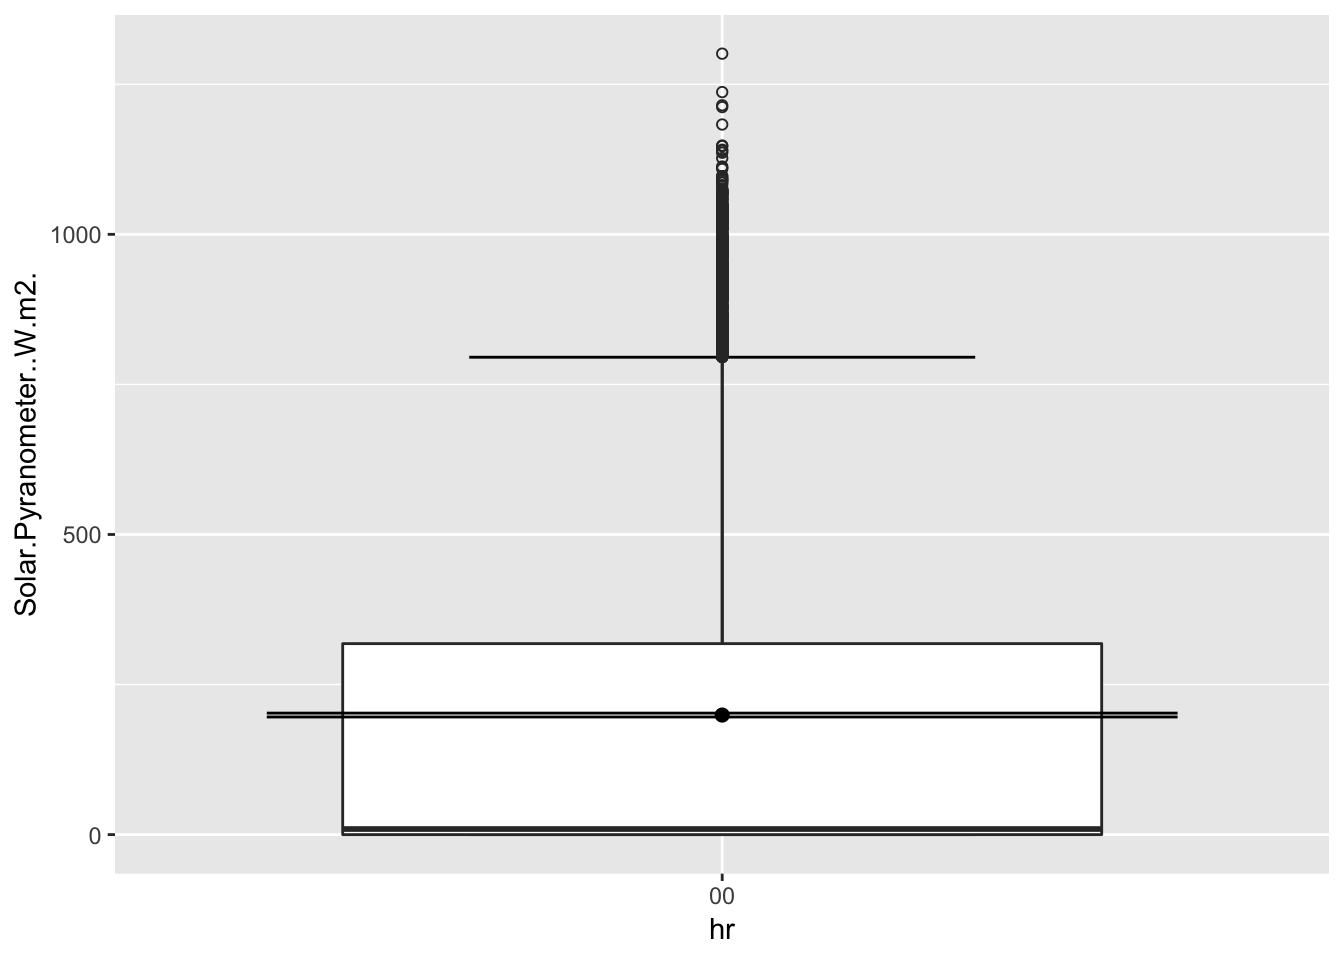
\includegraphics{Research_book_files/figure-latex/unnamed-chunk-7-1.pdf}

\begin{Shaded}
\begin{Highlighting}[]
\NormalTok{CampMuir_}\DecValTok{2017} \OperatorTok\StringTok{ }\KeywordTok{ggplot}\NormalTok{(}\KeywordTok{aes}\NormalTok{(date,Solar.Pyranometer..W.m2.)) }\OperatorTok{+}\StringTok{ }\KeywordTok{geom_point}\NormalTok{() }\OperatorTok{+}\StringTok{  }\KeywordTok{stat_smooth}\NormalTok{(}\DataTypeTok{se =} \OtherTok{TRUE}\NormalTok{) }\OperatorTok{+}\StringTok{ }\KeywordTok{ggtitle}\NormalTok{(}\StringTok{"Solar Radiation at CampMuir(10110 ft)"}\NormalTok{)}\OperatorTok{+}\StringTok{ }\KeywordTok{xlab}\NormalTok{(}\StringTok{"Date"}\NormalTok{) }\OperatorTok{+}\StringTok{ }\KeywordTok{ylab}\NormalTok{(}\StringTok{"Solar Irradiance(W/m^2)"}\NormalTok{)}
\end{Highlighting}
\end{Shaded}

\begin{verbatim}
## `geom_smooth()` using method = 'gam' and formula 'y ~ s(x, bs = "cs")'
\end{verbatim}

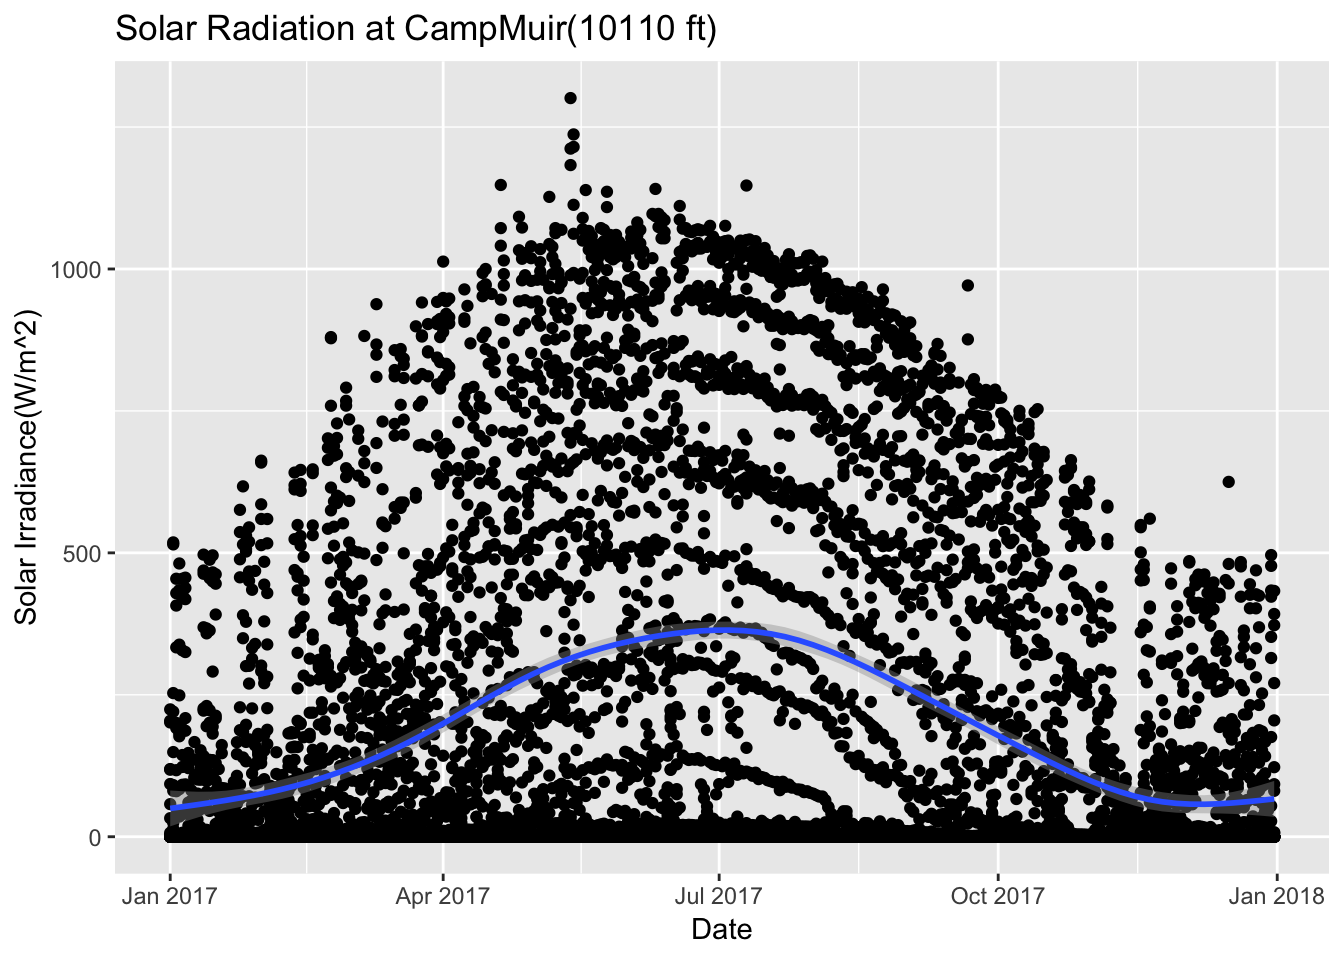
\includegraphics{Research_book_files/figure-latex/unnamed-chunk-7-2.pdf}

\begin{Shaded}
\begin{Highlighting}[]
\NormalTok{Sunriseupper_}\DecValTok{2017} \OperatorTok\StringTok{ }\KeywordTok{ggplot}\NormalTok{(}\KeywordTok{aes}\NormalTok{(date,Solar.Pyranometer..W.m2.)) }\OperatorTok{+}\StringTok{ }\KeywordTok{geom_point}\NormalTok{() }\OperatorTok{+}\StringTok{  }\KeywordTok{stat_smooth}\NormalTok{(}\DataTypeTok{se =} \OtherTok{TRUE}\NormalTok{) }\OperatorTok{+}\StringTok{ }\KeywordTok{ggtitle}\NormalTok{(}\StringTok{"Solar Radiation at Sunrise-Upper(6880 ft)"}\NormalTok{)}\OperatorTok{+}\StringTok{ }\KeywordTok{xlab}\NormalTok{(}\StringTok{"Date"}\NormalTok{) }\OperatorTok{+}\StringTok{ }\KeywordTok{ylab}\NormalTok{(}\StringTok{"Solar Irradiance(W/m^2)"}\NormalTok{)}
\end{Highlighting}
\end{Shaded}

\begin{verbatim}
## `geom_smooth()` using method = 'gam' and formula 'y ~ s(x, bs = "cs")'
\end{verbatim}

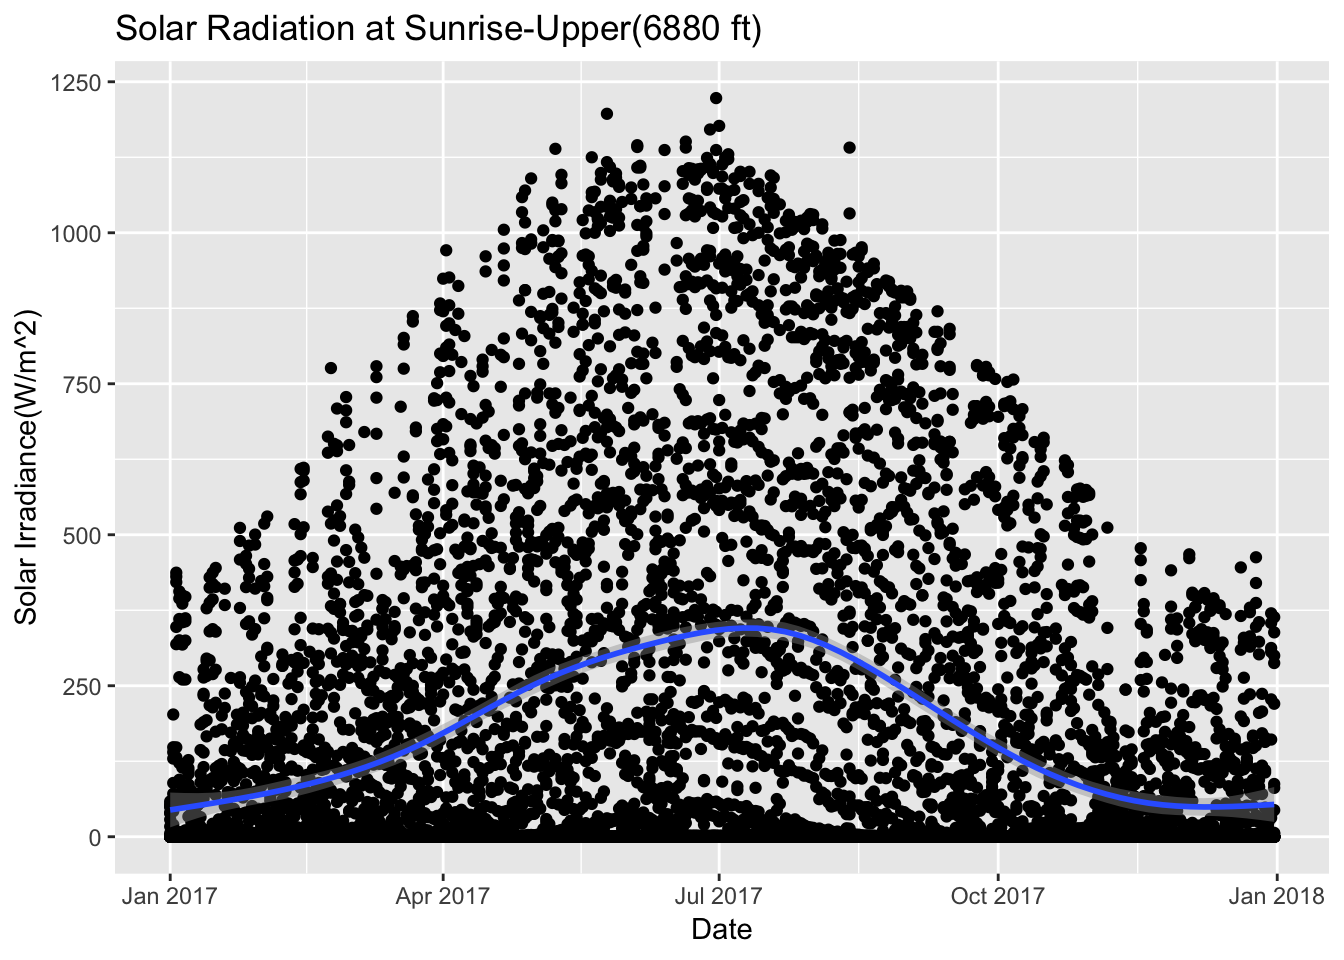
\includegraphics{Research_book_files/figure-latex/unnamed-chunk-7-3.pdf}

Feedback

Better to do it houry so that daily patterns do confound it. So, now we
have hourly solar radiation across all the sites.

\begin{Shaded}
\begin{Highlighting}[]
\NormalTok{## 4-28-2008}

\CommentTok{#}

\KeywordTok{ggplot}\NormalTok{(Paradise_}\DecValTok{2017}\NormalTok{, }\KeywordTok{aes}\NormalTok{(hr,Solar.Pyranometer..W.m2.))}\OperatorTok{+}
\StringTok{  }\KeywordTok{stat_boxplot}\NormalTok{( }\KeywordTok{aes}\NormalTok{(hr,Solar.Pyranometer..W.m2.), }
    \DataTypeTok{geom=}\StringTok{'errorbar'}\NormalTok{, }\DataTypeTok{linetype=}\DecValTok{1}\NormalTok{, }\DataTypeTok{width=}\FloatTok{0.5}\NormalTok{)}\OperatorTok{+}\StringTok{  }\CommentTok{#whiskers}
\StringTok{  }\KeywordTok{geom_boxplot}\NormalTok{( }\KeywordTok{aes}\NormalTok{(hr,Solar.Pyranometer..W.m2.),}\DataTypeTok{outlier.shape=}\DecValTok{1}\NormalTok{) }\OperatorTok{+}\StringTok{    }
\StringTok{  }\KeywordTok{stat_summary}\NormalTok{(}\DataTypeTok{fun.y=}\NormalTok{mean, }\DataTypeTok{geom=}\StringTok{"point"}\NormalTok{, }\DataTypeTok{size=}\DecValTok{2}\NormalTok{) }\OperatorTok{+}\StringTok{ }
\StringTok{  }\KeywordTok{stat_summary}\NormalTok{(}\DataTypeTok{fun.data =}\NormalTok{ mean_se, }\DataTypeTok{geom =} \StringTok{"errorbar"}\NormalTok{)}
\end{Highlighting}
\end{Shaded}

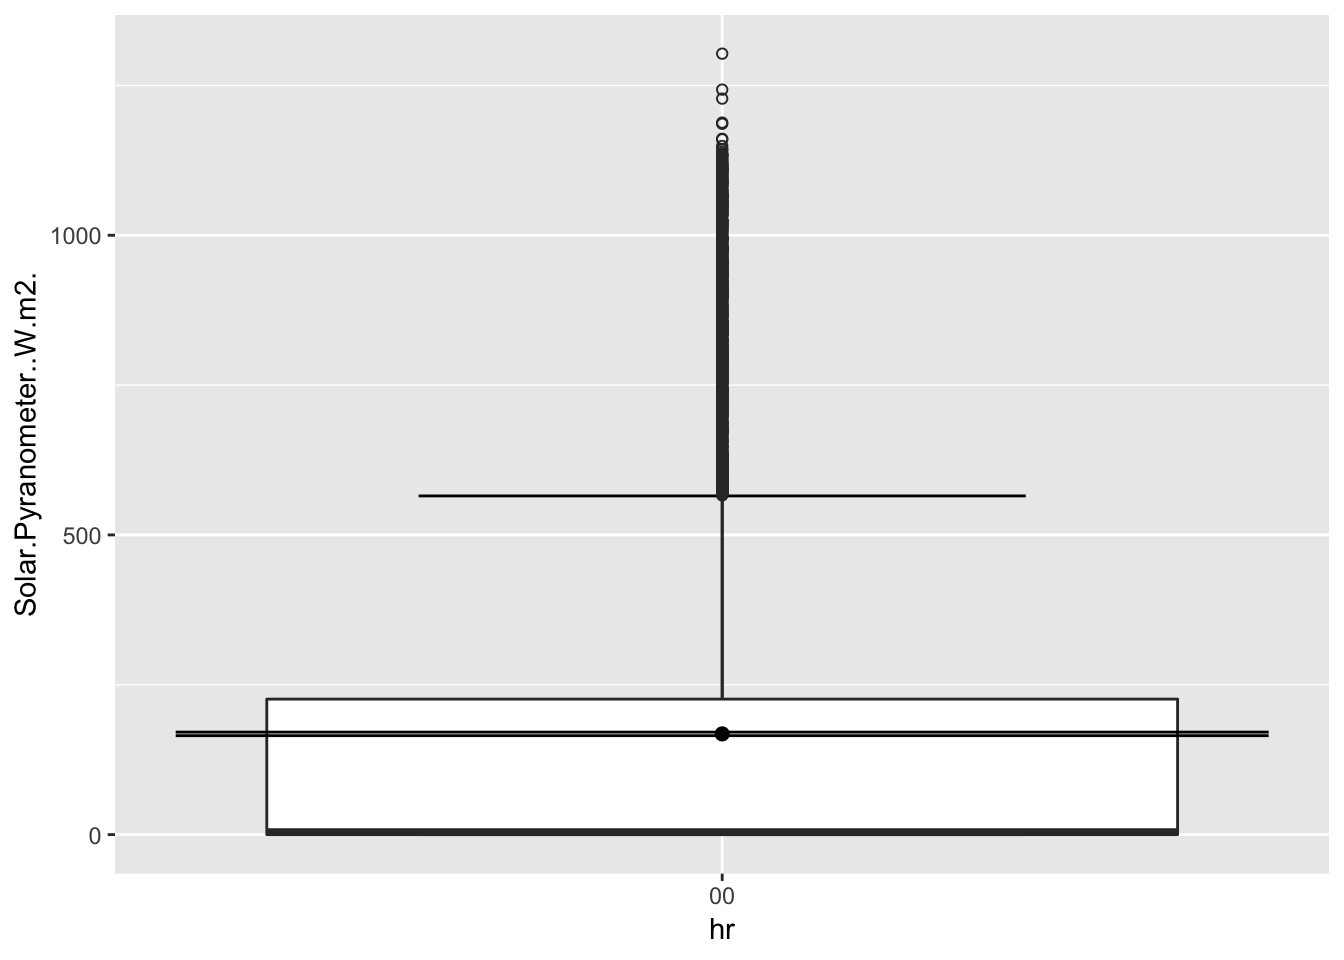
\includegraphics{Research_book_files/figure-latex/unnamed-chunk-8-1.pdf}

\begin{Shaded}
\begin{Highlighting}[]
 \KeywordTok{annotate}\NormalTok{(}\StringTok{"text"}\NormalTok{,}\DataTypeTok{x=}\DecValTok{20}\NormalTok{,}\DataTypeTok{y=}\DecValTok{55}\NormalTok{,}\DataTypeTok{label=}\StringTok{"wassup!"}\NormalTok{ , }\DataTypeTok{family=}\StringTok{"xkcd"}
\NormalTok{           )}
\end{Highlighting}
\end{Shaded}

\begin{verbatim}
## mapping: x = ~x, y = ~y 
## geom_text: na.rm = FALSE
## stat_identity: na.rm = FALSE
## position_identity
\end{verbatim}

\begin{Shaded}
\begin{Highlighting}[]
\NormalTok{## 4-28-2008}

\CommentTok{#}
\KeywordTok{ggplot}\NormalTok{(CampMuir_}\DecValTok{2017}\NormalTok{, }\KeywordTok{aes}\NormalTok{(hr,Solar.Pyranometer..W.m2.))}\OperatorTok{+}
\StringTok{  }\KeywordTok{stat_boxplot}\NormalTok{( }\KeywordTok{aes}\NormalTok{(hr,Solar.Pyranometer..W.m2.), }
    \DataTypeTok{geom=}\StringTok{'errorbar'}\NormalTok{, }\DataTypeTok{linetype=}\DecValTok{1}\NormalTok{, }\DataTypeTok{width=}\FloatTok{0.5}\NormalTok{)}\OperatorTok{+}\StringTok{  }\CommentTok{#whiskers}
\StringTok{  }\KeywordTok{geom_boxplot}\NormalTok{( }\KeywordTok{aes}\NormalTok{(hr,Solar.Pyranometer..W.m2.),}\DataTypeTok{outlier.shape=}\DecValTok{1}\NormalTok{) }\OperatorTok{+}\StringTok{    }
\StringTok{  }\KeywordTok{stat_summary}\NormalTok{(}\DataTypeTok{fun.y=}\NormalTok{mean, }\DataTypeTok{geom=}\StringTok{"point"}\NormalTok{, }\DataTypeTok{size=}\DecValTok{2}\NormalTok{) }\OperatorTok{+}\StringTok{ }
\StringTok{  }\KeywordTok{stat_summary}\NormalTok{(}\DataTypeTok{fun.data =}\NormalTok{ mean_se, }\DataTypeTok{geom =} \StringTok{"errorbar"}\NormalTok{)}
\end{Highlighting}
\end{Shaded}

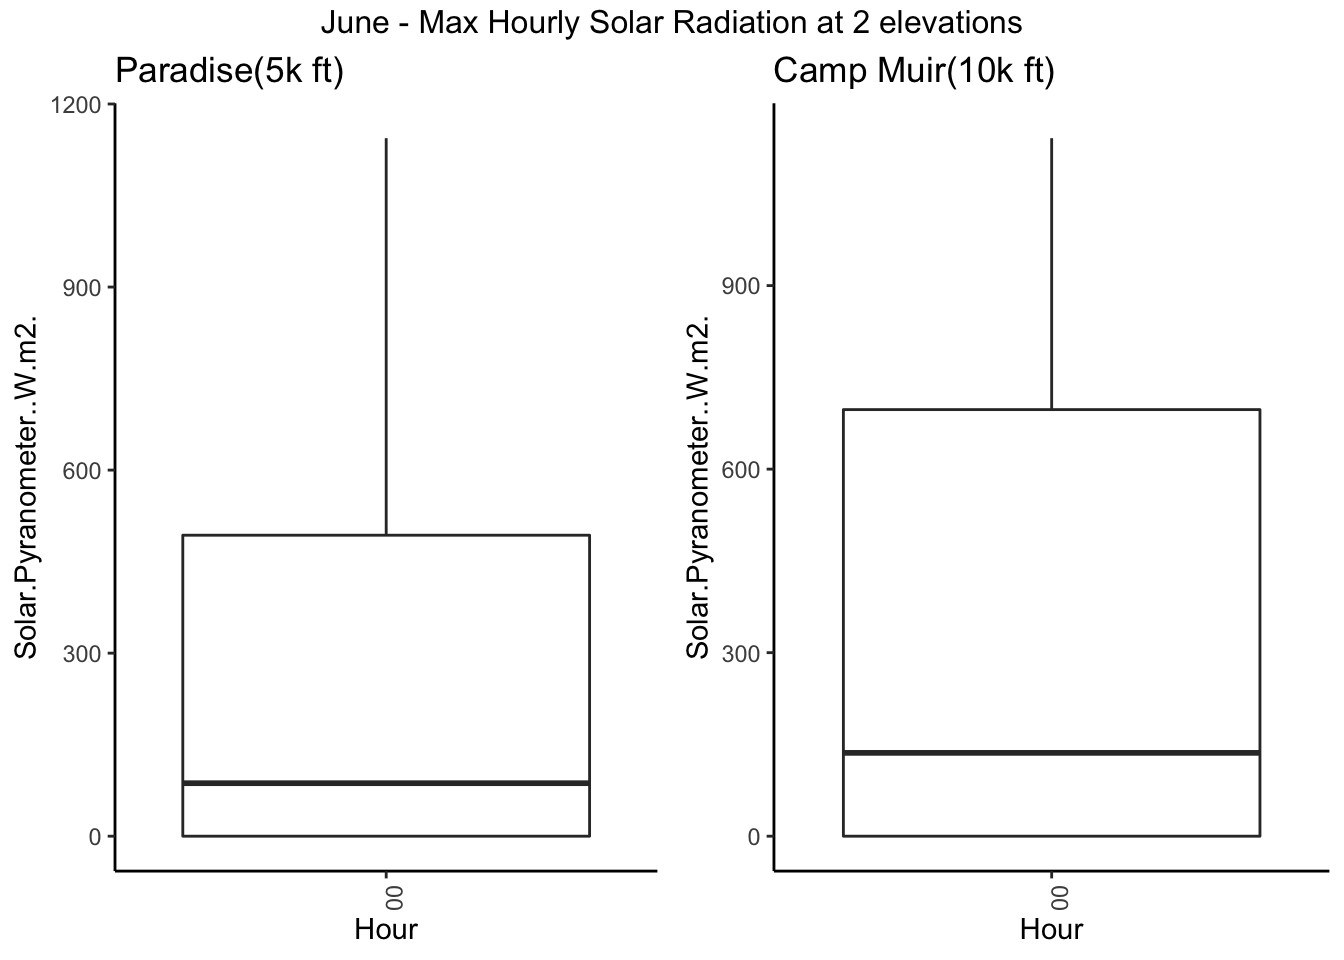
\includegraphics{Research_book_files/figure-latex/unnamed-chunk-9-1.pdf}

It does confirm that higher the sites, the solar radiation is slightly
higher.

\section{4-29-2008}\label{section-4}

Lets assume that solar radiation is infact more relevant at higher
elevations, so snowmelt would be at a faster rate at higher elevations.
Is snowmelt even at all the elevations ? Intuitively no as we often see
that peaks hold-on to snow longer. (Just aside discussion).

Here, the goal is to see if there is a difference in radiation recieved
at the sites. Reasoning being if the solar radiation recorded is
different, that would mean differemt growing degree days. Lets look for
June, July and August(JJA Summer). Summer solstice - June 21st.

\begin{Shaded}
\begin{Highlighting}[]
\NormalTok{## 4-29-2008}
\KeywordTok{library}\NormalTok{(gridExtra)}
\CommentTok{#}



\NormalTok{g1 <-}\StringTok{ }\NormalTok{Paradise_}\DecValTok{2017} \OperatorTok\StringTok{  }\KeywordTok{filter}\NormalTok{(month }\OperatorTok\StringTok{ }\KeywordTok{c}\NormalTok{(}\StringTok{'06'}\NormalTok{,}\StringTok{'07'}\NormalTok{,}\StringTok{'08'}\NormalTok{)) }\OperatorTok\StringTok{ }\KeywordTok{ggplot}\NormalTok{( }\KeywordTok{aes}\NormalTok{(hr,Solar.Pyranometer..W.m2.)) }\OperatorTok{+}\StringTok{ }\KeywordTok{geom_boxplot}\NormalTok{() }\OperatorTok{+}
\StringTok{    }\KeywordTok{stat_summary}\NormalTok{(}\DataTypeTok{colour =} \StringTok{"red"}\NormalTok{,}\DataTypeTok{size=}\FloatTok{0.5}\NormalTok{) }\OperatorTok{+}\StringTok{ }\KeywordTok{theme_classic}\NormalTok{() }\OperatorTok{+}\KeywordTok{theme}\NormalTok{(}\DataTypeTok{axis.text.x =} \KeywordTok{element_text}\NormalTok{(}\DataTypeTok{angle =} \DecValTok{90}\NormalTok{, }\DataTypeTok{hjust =} \DecValTok{1}\NormalTok{)) }\OperatorTok{+}\StringTok{     }\KeywordTok{xlab}\NormalTok{(}\StringTok{"Hour"}\NormalTok{) }\OperatorTok{+}\StringTok{ }\KeywordTok{ggtitle}\NormalTok{(}\StringTok{"Paradise(5k ft) "}\NormalTok{)}


\NormalTok{g2 <-}\StringTok{ }\NormalTok{CampMuir_}\DecValTok{2017} \OperatorTok\StringTok{  }\KeywordTok{filter}\NormalTok{(month }\OperatorTok\StringTok{ }\KeywordTok{c}\NormalTok{(}\StringTok{'06'}\NormalTok{,}\StringTok{'07'}\NormalTok{,}\StringTok{'08'}\NormalTok{)) }\OperatorTok\StringTok{ }\KeywordTok{ggplot}\NormalTok{( }\KeywordTok{aes}\NormalTok{(hr,Solar.Pyranometer..W.m2.)) }\OperatorTok{+}\StringTok{ }\KeywordTok{geom_boxplot}\NormalTok{() }\OperatorTok{+}
\StringTok{    }\KeywordTok{stat_summary}\NormalTok{(}\DataTypeTok{colour =} \StringTok{"red"}\NormalTok{,}\DataTypeTok{size=}\FloatTok{0.5}\NormalTok{) }\OperatorTok{+}\StringTok{ }\KeywordTok{theme_classic}\NormalTok{() }\OperatorTok{+}\KeywordTok{theme}\NormalTok{(}\DataTypeTok{axis.text.x =} \KeywordTok{element_text}\NormalTok{(}\DataTypeTok{angle =} \DecValTok{90}\NormalTok{, }\DataTypeTok{hjust =} \DecValTok{1}\NormalTok{)) }\OperatorTok{+}\StringTok{     }\KeywordTok{xlab}\NormalTok{(}\StringTok{"Hour"}\NormalTok{) }\OperatorTok{+}\StringTok{ }\KeywordTok{ggtitle}\NormalTok{(}\StringTok{"Camp Muir(10k ft) "}\NormalTok{)}


\KeywordTok{grid.arrange}\NormalTok{(g1, g2,}\DataTypeTok{ncol=}\DecValTok{2}\NormalTok{, }\DataTypeTok{top =} \StringTok{"JJA - Mean Hourly Solar Radiation at 2 elevations"}\NormalTok{)}
\end{Highlighting}
\end{Shaded}

\begin{verbatim}
## No summary function supplied, defaulting to `mean_se()
## No summary function supplied, defaulting to `mean_se()
\end{verbatim}

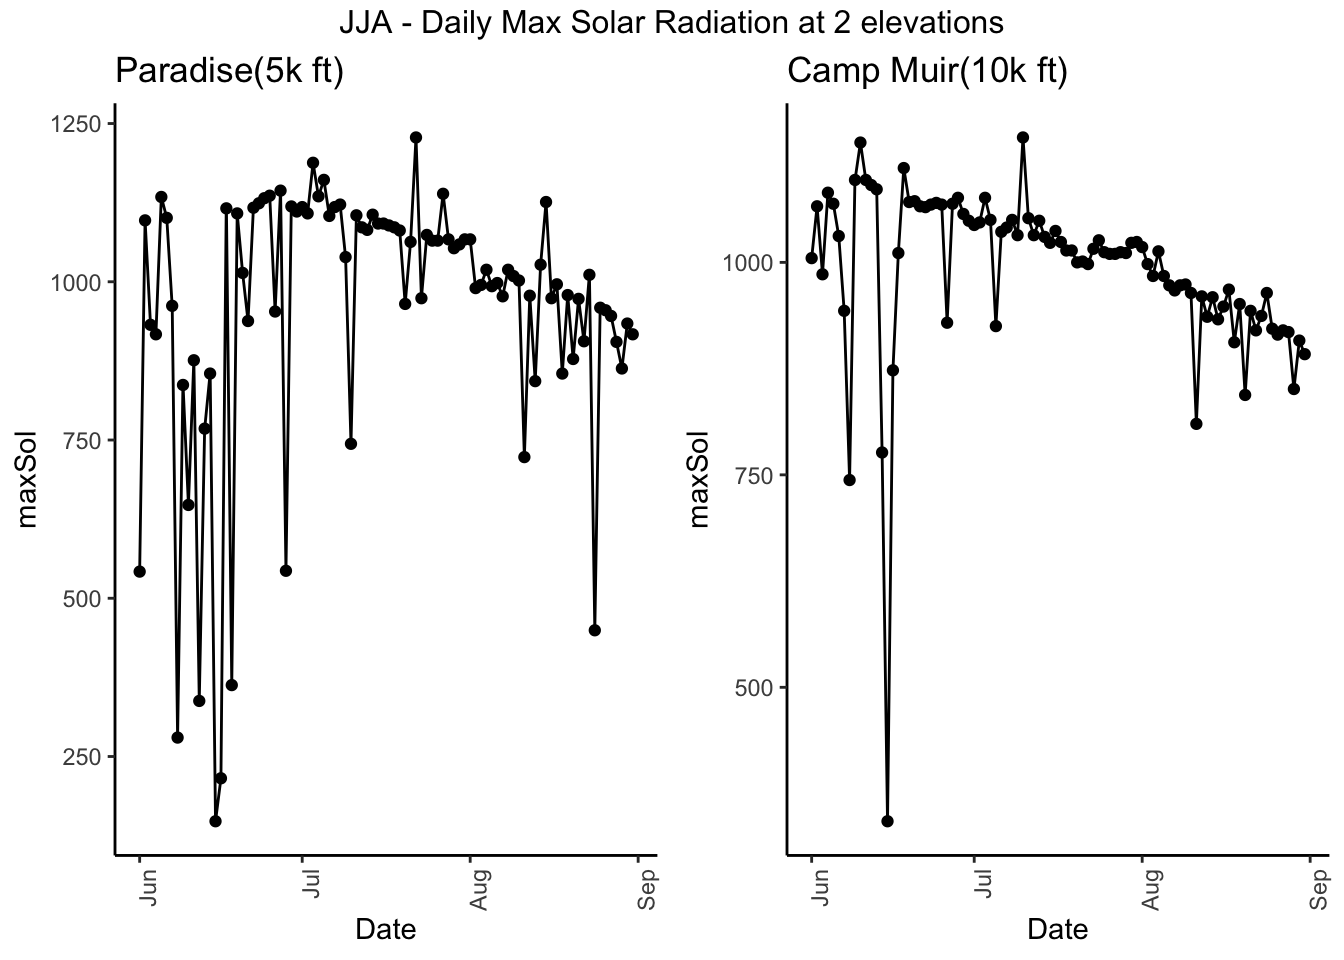
\includegraphics{Research_book_files/figure-latex/unnamed-chunk-10-1.pdf}

\begin{Shaded}
\begin{Highlighting}[]
\NormalTok{## 4-29-2008}
\KeywordTok{library}\NormalTok{(gridExtra)}
\CommentTok{#}



\NormalTok{g3 <-}\StringTok{ }\NormalTok{Paradise_}\DecValTok{2017} \OperatorTok\StringTok{  }\KeywordTok{filter}\NormalTok{(month }\OperatorTok\StringTok{ }\KeywordTok{c}\NormalTok{(}\StringTok{'06'}\NormalTok{)) }\OperatorTok\StringTok{ }\KeywordTok{ggplot}\NormalTok{( }\KeywordTok{aes}\NormalTok{(hr,Solar.Pyranometer..W.m2.)) }\OperatorTok{+}\StringTok{ }\KeywordTok{geom_boxplot}\NormalTok{() }\OperatorTok{+}
\StringTok{    }\KeywordTok{theme_classic}\NormalTok{() }\OperatorTok{+}\KeywordTok{theme}\NormalTok{(}\DataTypeTok{axis.text.x =} \KeywordTok{element_text}\NormalTok{(}\DataTypeTok{angle =} \DecValTok{90}\NormalTok{, }\DataTypeTok{hjust =} \DecValTok{1}\NormalTok{)) }\OperatorTok{+}\StringTok{     }\KeywordTok{xlab}\NormalTok{(}\StringTok{"Hour"}\NormalTok{) }\OperatorTok{+}\StringTok{ }\KeywordTok{ggtitle}\NormalTok{(}\StringTok{"Paradise(5k ft) "}\NormalTok{)}


\NormalTok{g4 <-}\StringTok{ }\NormalTok{CampMuir_}\DecValTok{2017} \OperatorTok\StringTok{  }\KeywordTok{filter}\NormalTok{(month }\OperatorTok\StringTok{ }\KeywordTok{c}\NormalTok{(}\StringTok{'06'}\NormalTok{)) }\OperatorTok\StringTok{ }\KeywordTok{ggplot}\NormalTok{( }\KeywordTok{aes}\NormalTok{(hr,Solar.Pyranometer..W.m2.)) }\OperatorTok{+}\StringTok{ }\KeywordTok{geom_boxplot}\NormalTok{() }\OperatorTok{+}
\StringTok{   }\KeywordTok{theme_classic}\NormalTok{() }\OperatorTok{+}\KeywordTok{theme}\NormalTok{(}\DataTypeTok{axis.text.x =} \KeywordTok{element_text}\NormalTok{(}\DataTypeTok{angle =} \DecValTok{90}\NormalTok{, }\DataTypeTok{hjust =} \DecValTok{1}\NormalTok{)) }\OperatorTok{+}\StringTok{     }\KeywordTok{xlab}\NormalTok{(}\StringTok{"Hour"}\NormalTok{) }\OperatorTok{+}\StringTok{ }\KeywordTok{ggtitle}\NormalTok{(}\StringTok{"Camp Muir(10k ft) "}\NormalTok{)}


\KeywordTok{grid.arrange}\NormalTok{(g3, g4,}\DataTypeTok{ncol=}\DecValTok{2}\NormalTok{, }\DataTypeTok{top =} \StringTok{"June - Max Hourly Solar Radiation at 2 elevations"}\NormalTok{)}
\end{Highlighting}
\end{Shaded}

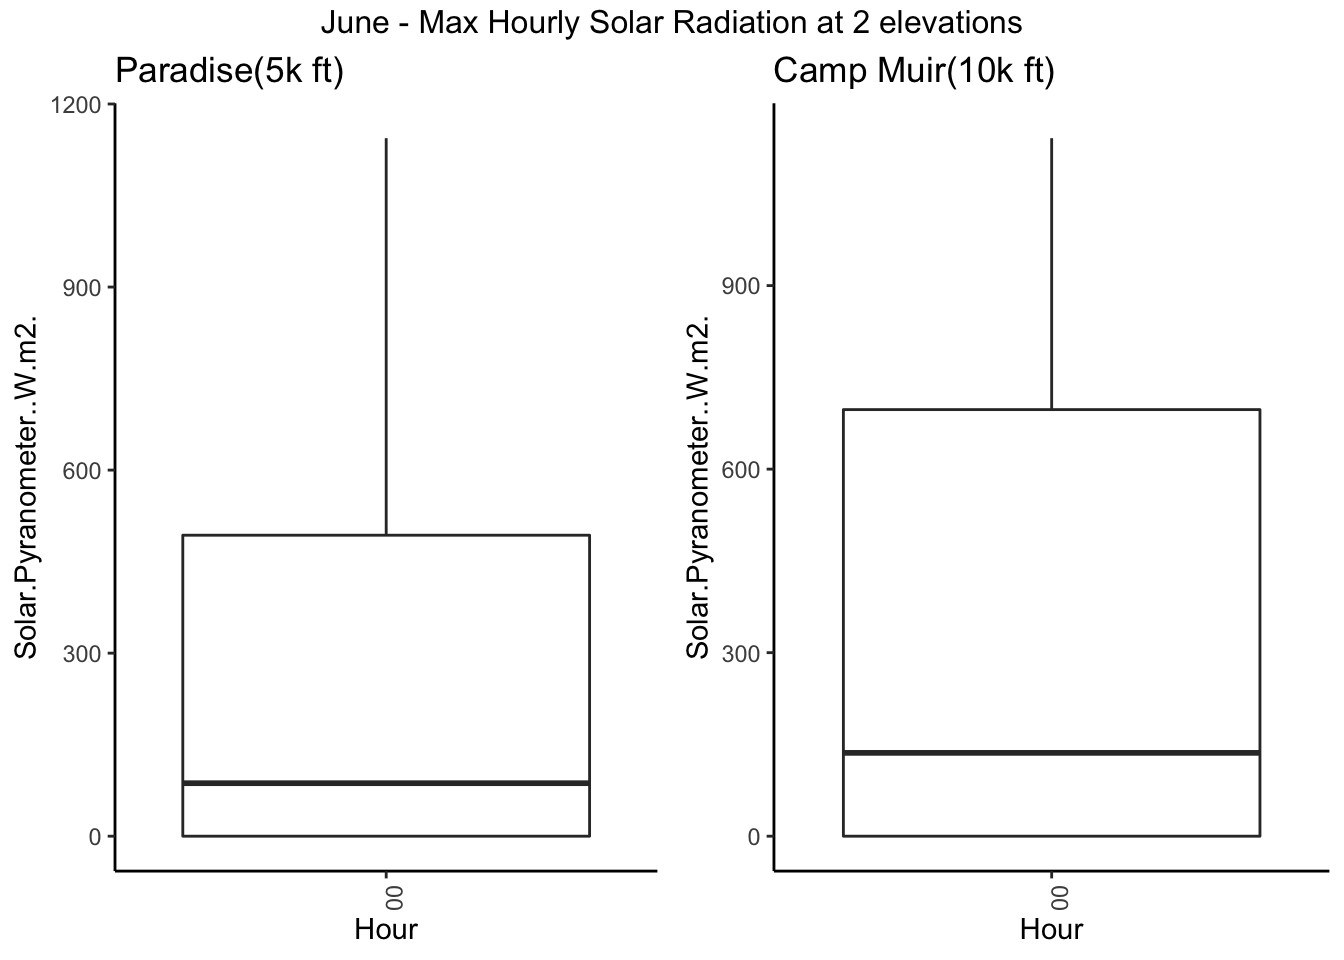
\includegraphics{Research_book_files/figure-latex/unnamed-chunk-11-1.pdf}

\begin{Shaded}
\begin{Highlighting}[]
\CommentTok{#ggplotly()}
\end{Highlighting}
\end{Shaded}

Lets check the daily max for each day in summer(JJA)

\begin{Shaded}
\begin{Highlighting}[]
\NormalTok{## 4-29-2008}
\KeywordTok{library}\NormalTok{(gridExtra)}
\CommentTok{#}



\NormalTok{g5 <-}\StringTok{ }\NormalTok{Paradise_}\DecValTok{2017} \OperatorTok\StringTok{  }\KeywordTok{filter}\NormalTok{(month }\OperatorTok\StringTok{ }\KeywordTok{c}\NormalTok{(}\StringTok{'06'}\NormalTok{,}\StringTok{'07'}\NormalTok{,}\StringTok{'08'}\NormalTok{)) }\OperatorTok\StringTok{ }\NormalTok{dplyr}\OperatorTok{::}\KeywordTok{group_by}\NormalTok{(date) }\OperatorTok
\StringTok{  }\NormalTok{dplyr}\OperatorTok{::}\KeywordTok{summarise}\NormalTok{(}\DataTypeTok{maxSol =} \KeywordTok{max}\NormalTok{(Solar.Pyranometer..W.m2.)) }\OperatorTok
\StringTok{  }\KeywordTok{ggplot}\NormalTok{( }\KeywordTok{aes}\NormalTok{(date,maxSol)) }\OperatorTok{+}\StringTok{ }\KeywordTok{geom_point}\NormalTok{() }\OperatorTok{+}\StringTok{ }\KeywordTok{geom_line}\NormalTok{() }\OperatorTok{+}
\StringTok{    }\KeywordTok{theme_classic}\NormalTok{() }\OperatorTok{+}\KeywordTok{theme}\NormalTok{(}\DataTypeTok{axis.text.x =} \KeywordTok{element_text}\NormalTok{(}\DataTypeTok{angle =} \DecValTok{90}\NormalTok{, }\DataTypeTok{hjust =} \DecValTok{1}\NormalTok{)) }\OperatorTok{+}\StringTok{     }\KeywordTok{xlab}\NormalTok{(}\StringTok{"Date"}\NormalTok{) }\OperatorTok{+}\StringTok{ }\KeywordTok{ggtitle}\NormalTok{(}\StringTok{"Paradise(5k ft) "}\NormalTok{)}


\NormalTok{g6 <-}\StringTok{ }\NormalTok{CampMuir_}\DecValTok{2017} \OperatorTok\StringTok{  }\KeywordTok{filter}\NormalTok{(month }\OperatorTok\StringTok{ }\KeywordTok{c}\NormalTok{(}\StringTok{'06'}\NormalTok{,}\StringTok{'07'}\NormalTok{,}\StringTok{'08'}\NormalTok{)) }\OperatorTok\StringTok{ }\NormalTok{dplyr}\OperatorTok{::}\KeywordTok{group_by}\NormalTok{(date) }\OperatorTok
\StringTok{  }\NormalTok{dplyr}\OperatorTok{::}\KeywordTok{summarise}\NormalTok{(}\DataTypeTok{maxSol =} \KeywordTok{max}\NormalTok{(Solar.Pyranometer..W.m2.)) }\OperatorTok
\StringTok{  }\KeywordTok{ggplot}\NormalTok{( }\KeywordTok{aes}\NormalTok{(date,maxSol)) }\OperatorTok{+}\StringTok{ }\KeywordTok{geom_point}\NormalTok{() }\OperatorTok{+}\StringTok{  }\KeywordTok{geom_line}\NormalTok{() }\OperatorTok{+}
\StringTok{    }\KeywordTok{theme_classic}\NormalTok{() }\OperatorTok{+}\KeywordTok{theme}\NormalTok{(}\DataTypeTok{axis.text.x =} \KeywordTok{element_text}\NormalTok{(}\DataTypeTok{angle =} \DecValTok{90}\NormalTok{, }\DataTypeTok{hjust =} \DecValTok{1}\NormalTok{)) }\OperatorTok{+}\StringTok{     }\KeywordTok{xlab}\NormalTok{(}\StringTok{"Date"}\NormalTok{) }\OperatorTok{+}\StringTok{ }\KeywordTok{ggtitle}\NormalTok{(}\StringTok{"Camp Muir(10k ft) "}\NormalTok{)}


\KeywordTok{grid.arrange}\NormalTok{(g5, g6,}\DataTypeTok{ncol=}\DecValTok{2}\NormalTok{, }\DataTypeTok{top =} \StringTok{"JJA - Daily Max Solar Radiation at 2 elevations"}\NormalTok{)}
\end{Highlighting}
\end{Shaded}

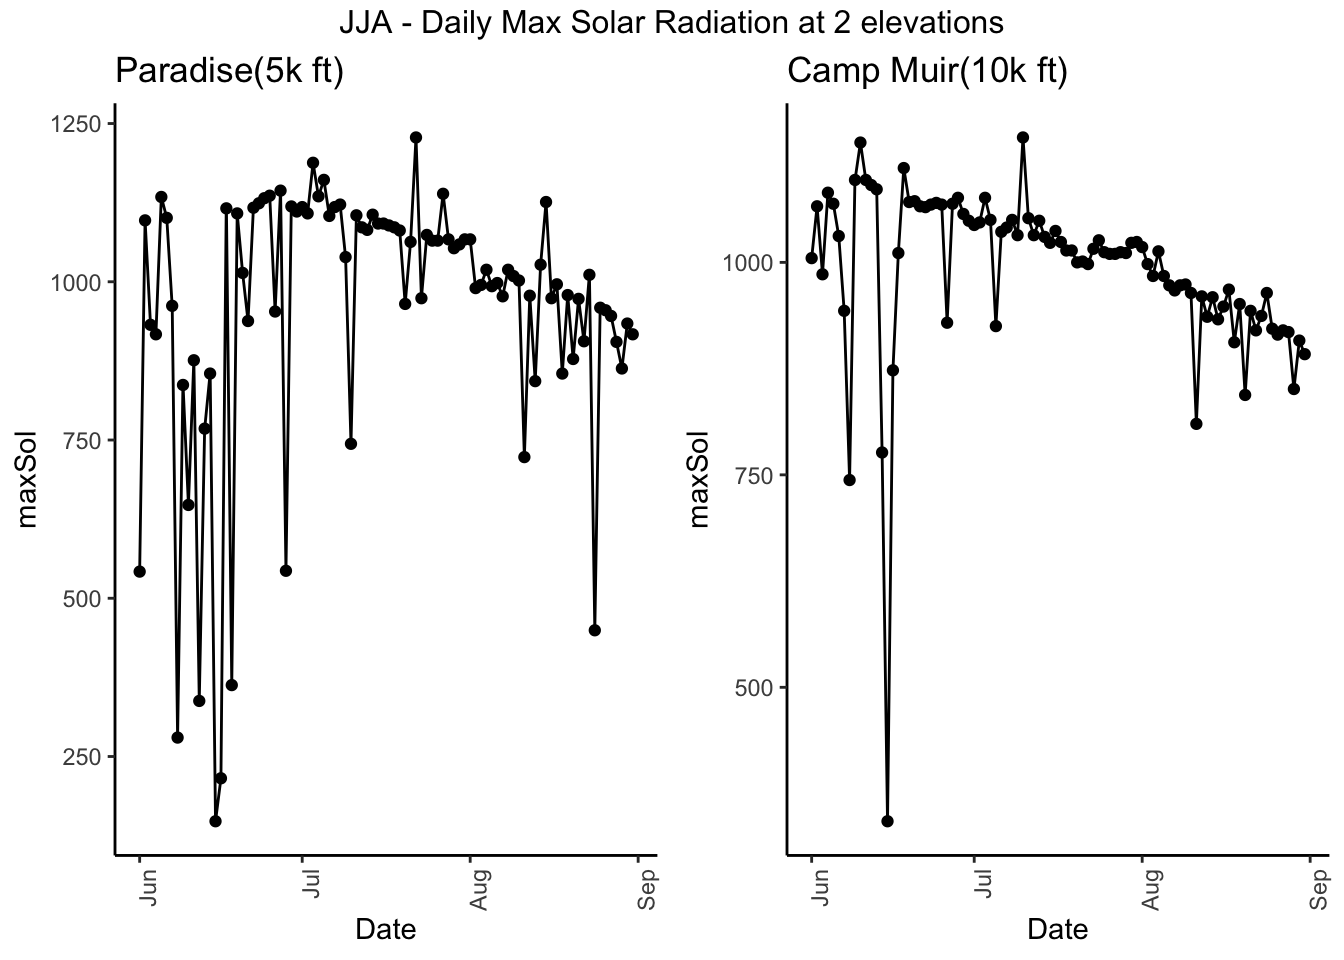
\includegraphics{Research_book_files/figure-latex/unnamed-chunk-12-1.pdf}

\begin{Shaded}
\begin{Highlighting}[]
\CommentTok{#ggplotly()}
\end{Highlighting}
\end{Shaded}

Compare wind and solar at two sites

\begin{Shaded}
\begin{Highlighting}[]
\NormalTok{## 4-29-2008}
\KeywordTok{library}\NormalTok{(gridExtra)}
\CommentTok{#}



\NormalTok{g5 <-}\StringTok{ }\NormalTok{Paradise_}\DecValTok{2017} \OperatorTok\StringTok{  }\KeywordTok{filter}\NormalTok{(month }\OperatorTok\StringTok{ }\KeywordTok{c}\NormalTok{(}\StringTok{'06'}\NormalTok{,}\StringTok{'07'}\NormalTok{,}\StringTok{'08'}\NormalTok{)) }\OperatorTok\StringTok{ }\NormalTok{dplyr}\OperatorTok{::}\KeywordTok{group_by}\NormalTok{(date) }\OperatorTok
\StringTok{  }\NormalTok{dplyr}\OperatorTok{::}\KeywordTok{summarise}\NormalTok{(}\DataTypeTok{maxSol =} \KeywordTok{max}\NormalTok{(Solar.Pyranometer..W.m2.),}\DataTypeTok{maxWind =} \KeywordTok{max}\NormalTok{(Wind.Speed.Average..mph.)) }\OperatorTok
\StringTok{  }\KeywordTok{ggplot}\NormalTok{() }\OperatorTok{+}\StringTok{ }\KeywordTok{geom_line}\NormalTok{(}\KeywordTok{aes}\NormalTok{(date,}\KeywordTok{log}\NormalTok{(maxSol),}\DataTypeTok{color=}\StringTok{'log Solar(W/m^2)'}\NormalTok{) ) }\OperatorTok{+}\StringTok{ }\KeywordTok{geom_line}\NormalTok{(}\KeywordTok{aes}\NormalTok{(date,maxWind,}\DataTypeTok{color=}\StringTok{'Wind(m/h)'}\NormalTok{)) }\OperatorTok{+}
\StringTok{    }\KeywordTok{theme_classic}\NormalTok{() }\OperatorTok{+}\KeywordTok{theme}\NormalTok{(}\DataTypeTok{axis.text.x =} \KeywordTok{element_text}\NormalTok{(}\DataTypeTok{angle =} \DecValTok{90}\NormalTok{, }\DataTypeTok{hjust =} \DecValTok{1}\NormalTok{)) }\OperatorTok{+}\StringTok{     }\KeywordTok{xlab}\NormalTok{(}\StringTok{"Date"}\NormalTok{) }\OperatorTok{+}\StringTok{ }\KeywordTok{ylab}\NormalTok{(}\StringTok{""}\NormalTok{) }\OperatorTok{+}\StringTok{ }\KeywordTok{ggtitle}\NormalTok{(}\StringTok{"Paradise(5k ft) "}\NormalTok{) }\OperatorTok{+}\StringTok{ }\KeywordTok{scale_color_discrete}\NormalTok{(}\DataTypeTok{name=}\StringTok{"Variable"}\NormalTok{)}


\NormalTok{g6 <-}\StringTok{ }\NormalTok{CampMuir_}\DecValTok{2017} \OperatorTok\StringTok{  }\KeywordTok{filter}\NormalTok{(month }\OperatorTok\StringTok{ }\KeywordTok{c}\NormalTok{(}\StringTok{'06'}\NormalTok{,}\StringTok{'07'}\NormalTok{,}\StringTok{'08'}\NormalTok{)) }\OperatorTok\StringTok{ }\NormalTok{dplyr}\OperatorTok{::}\KeywordTok{group_by}\NormalTok{(date) }\OperatorTok
\StringTok{  }\NormalTok{dplyr}\OperatorTok{::}\KeywordTok{summarise}\NormalTok{(}\DataTypeTok{maxSol =} \KeywordTok{max}\NormalTok{(Solar.Pyranometer..W.m2.),}\DataTypeTok{maxWind =} \KeywordTok{max}\NormalTok{(Wind.Speed.Average..mph.)) }\OperatorTok
\StringTok{  }\KeywordTok{ggplot}\NormalTok{() }\OperatorTok{+}\StringTok{ }\KeywordTok{geom_line}\NormalTok{(}\KeywordTok{aes}\NormalTok{(date,}\KeywordTok{log}\NormalTok{(maxSol),}\DataTypeTok{color=}\StringTok{'log Solar(W/m^2)'}\NormalTok{) ) }\OperatorTok{+}\StringTok{ }\KeywordTok{geom_line}\NormalTok{(}\KeywordTok{aes}\NormalTok{(date,maxWind,}\DataTypeTok{color=}\StringTok{'Wind(m/h)'}\NormalTok{)) }\OperatorTok{+}
\StringTok{    }\KeywordTok{theme_classic}\NormalTok{() }\OperatorTok{+}\KeywordTok{theme}\NormalTok{(}\DataTypeTok{axis.text.x =} \KeywordTok{element_text}\NormalTok{(}\DataTypeTok{angle =} \DecValTok{90}\NormalTok{, }\DataTypeTok{hjust =} \DecValTok{1}\NormalTok{)) }\OperatorTok{+}\StringTok{     }\KeywordTok{xlab}\NormalTok{(}\StringTok{"Date"}\NormalTok{) }\OperatorTok{+}\StringTok{ }\KeywordTok{ylab}\NormalTok{(}\StringTok{""}\NormalTok{) }\OperatorTok{+}\StringTok{ }\KeywordTok{ggtitle}\NormalTok{(}\StringTok{"Camp Muir(10k ft) "}\NormalTok{) }\OperatorTok{+}\StringTok{ }\KeywordTok{scale_color_discrete}\NormalTok{(}\DataTypeTok{name=}\StringTok{"Variable"}\NormalTok{)}


\KeywordTok{grid.arrange}\NormalTok{(g5, g6,}\DataTypeTok{ncol=}\DecValTok{2}\NormalTok{, }\DataTypeTok{top =} \StringTok{"JJA - Daily Max Solar and Max Wind(Avg)  at 2 elevations"}\NormalTok{)}
\end{Highlighting}
\end{Shaded}

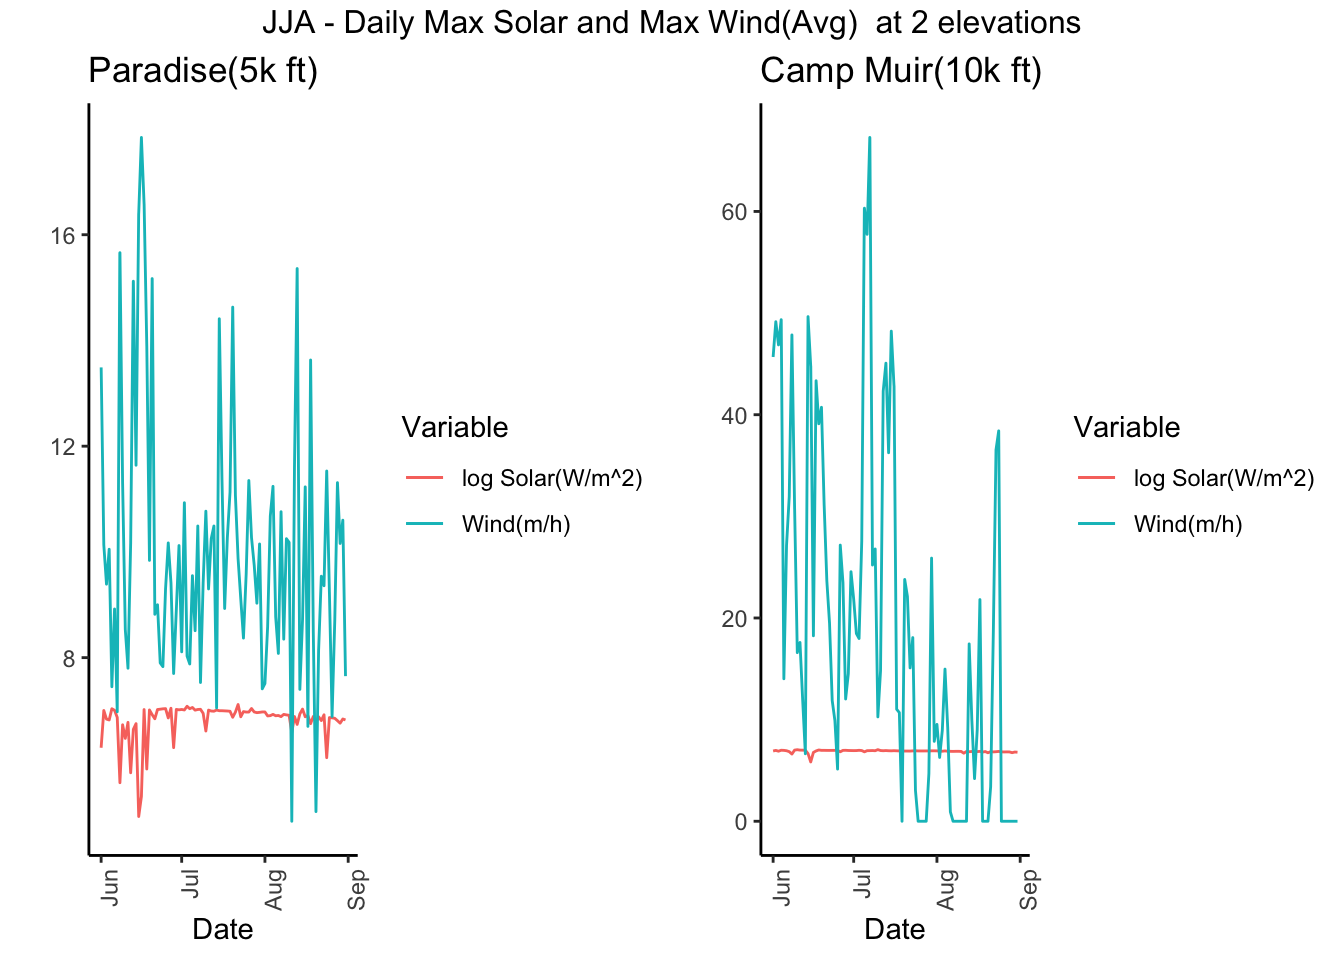
\includegraphics{Research_book_files/figure-latex/unnamed-chunk-13-1.pdf}

\begin{Shaded}
\begin{Highlighting}[]
\CommentTok{#ggplotly()}
\end{Highlighting}
\end{Shaded}

\section{5-21-2018}\label{section-5}

Wrangle the microclimate data

\begin{Shaded}
\begin{Highlighting}[]
\NormalTok{## 5-21-2018}
\NormalTok{mclim_}\DecValTok{2018}\NormalTok{<-}\StringTok{ }\KeywordTok{read.csv}\NormalTok{(}\StringTok{'./data/DATALOG.5.15.2018.csv'}\NormalTok{)}

\CommentTok{#ggplotly()}
\end{Highlighting}
\end{Shaded}

Look at the data

\begin{Shaded}
\begin{Highlighting}[]
\NormalTok{## 5-21-2018}
\KeywordTok{str}\NormalTok{(mclim_}\DecValTok{2018}\NormalTok{)}
\end{Highlighting}
\end{Shaded}

\begin{verbatim}
## 'data.frame':    326489 obs. of  4 variables:
##  $ X2018.5.8.16.35.01: Factor w/ 73277 levels "2018/5/10 0:00:03",..: 60336 60336 60336 60336 60336 60337 60338 60338 60338 60338 ...
##  $ X28CF6F0400008059 : Factor w/ 6 levels "287F5B04000080C5",..: 1 5 6 4 3 2 1 5 6 4 ...
##  $ X14.31            : num  14.8 14.4 14.8 14.3 14.1 ...
##  $ X4.14             : num  4.14 4.14 4.14 4.14 4.14 4.14 4.14 4.14 4.14 4.14 ...
\end{verbatim}

\begin{Shaded}
\begin{Highlighting}[]
\KeywordTok{names}\NormalTok{(mclim_}\DecValTok{2018}\NormalTok{) <-}\StringTok{ }\KeywordTok{c}\NormalTok{(}\StringTok{'time'}\NormalTok{,}\StringTok{'nodeid'}\NormalTok{,}\StringTok{'temp'}\NormalTok{,}\StringTok{'batt'}\NormalTok{)}
\NormalTok{mclim_}\DecValTok{2018}\OperatorTok{$}\NormalTok{time <-}\StringTok{ }\KeywordTok{as.POSIXct}\NormalTok{(mclim_}\DecValTok{2018}\OperatorTok{$}\NormalTok{time, }\StringTok{"%Y/%m/%d %H:%M:%S"}\NormalTok{)}
\end{Highlighting}
\end{Shaded}

Add Hour, month and day

\begin{Shaded}
\begin{Highlighting}[]
\NormalTok{## 5-21-2018}
\NormalTok{mclim_}\DecValTok{2018}\OperatorTok{$}\NormalTok{hr <-}\StringTok{ }\KeywordTok{hour}\NormalTok{(mclim_}\DecValTok{2018}\OperatorTok{$}\NormalTok{time)}
\NormalTok{mclim_}\DecValTok{2018}\OperatorTok{$}\NormalTok{day <-}\StringTok{ }\KeywordTok{day}\NormalTok{(mclim_}\DecValTok{2018}\OperatorTok{$}\NormalTok{time)}
\NormalTok{mclim_}\DecValTok{2018}\OperatorTok{$}\NormalTok{month<-}\StringTok{ }\KeywordTok{month}\NormalTok{(mclim_}\DecValTok{2018}\OperatorTok{$}\NormalTok{time)}
\end{Highlighting}
\end{Shaded}

Basic plot (May 10th)

\begin{Shaded}
\begin{Highlighting}[]
\NormalTok{## 5-21-2018}
\NormalTok{mclim_}\DecValTok{2018} \OperatorTok\StringTok{ }\KeywordTok{filter}\NormalTok{(}\KeywordTok{day}\NormalTok{(time) }\OperatorTok\StringTok{ '10'}\NormalTok{) }\OperatorTok
\KeywordTok{ggplot}\NormalTok{( }\KeywordTok{aes}\NormalTok{(time,temp,}\DataTypeTok{color =}\NormalTok{ nodeid)) }\OperatorTok{+}\StringTok{ }\KeywordTok{geom_line}\NormalTok{() }\OperatorTok{+}\StringTok{ }\KeywordTok{theme_minimal}\NormalTok{()}
\end{Highlighting}
\end{Shaded}

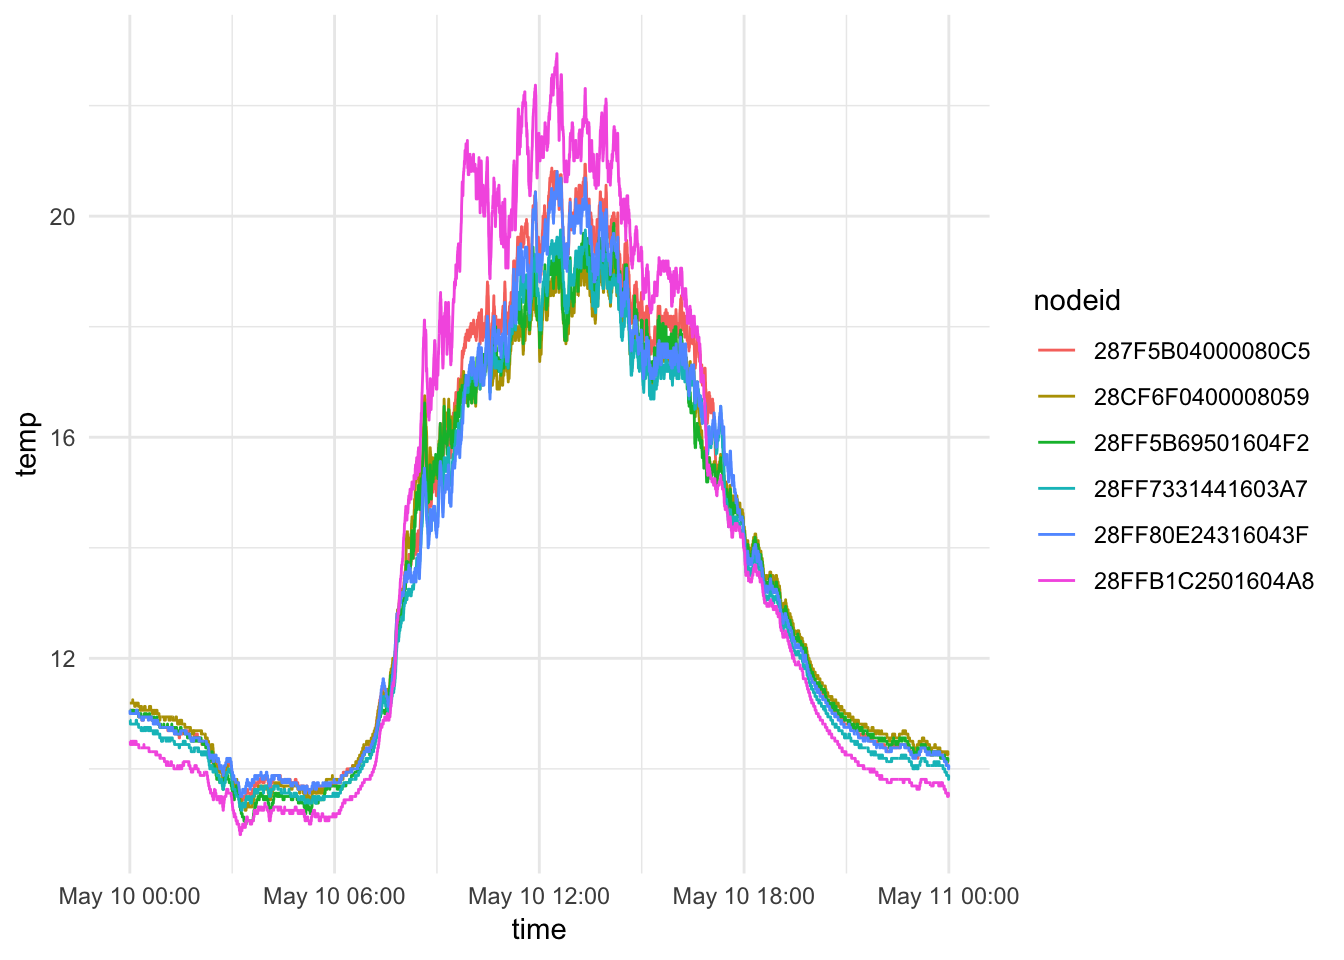
\includegraphics{Research_book_files/figure-latex/unnamed-chunk-17-1.pdf}

\begin{Shaded}
\begin{Highlighting}[]
\CommentTok{#ggplotly()}
\end{Highlighting}
\end{Shaded}

Whole week

\begin{Shaded}
\begin{Highlighting}[]
\NormalTok{## 5-21-2018}
\NormalTok{mclim_}\DecValTok{2018} \OperatorTok\StringTok{ }
\KeywordTok{ggplot}\NormalTok{( }\KeywordTok{aes}\NormalTok{(time,temp,}\DataTypeTok{color =}\NormalTok{ nodeid)) }\OperatorTok{+}\StringTok{ }\KeywordTok{geom_line}\NormalTok{()}
\end{Highlighting}
\end{Shaded}

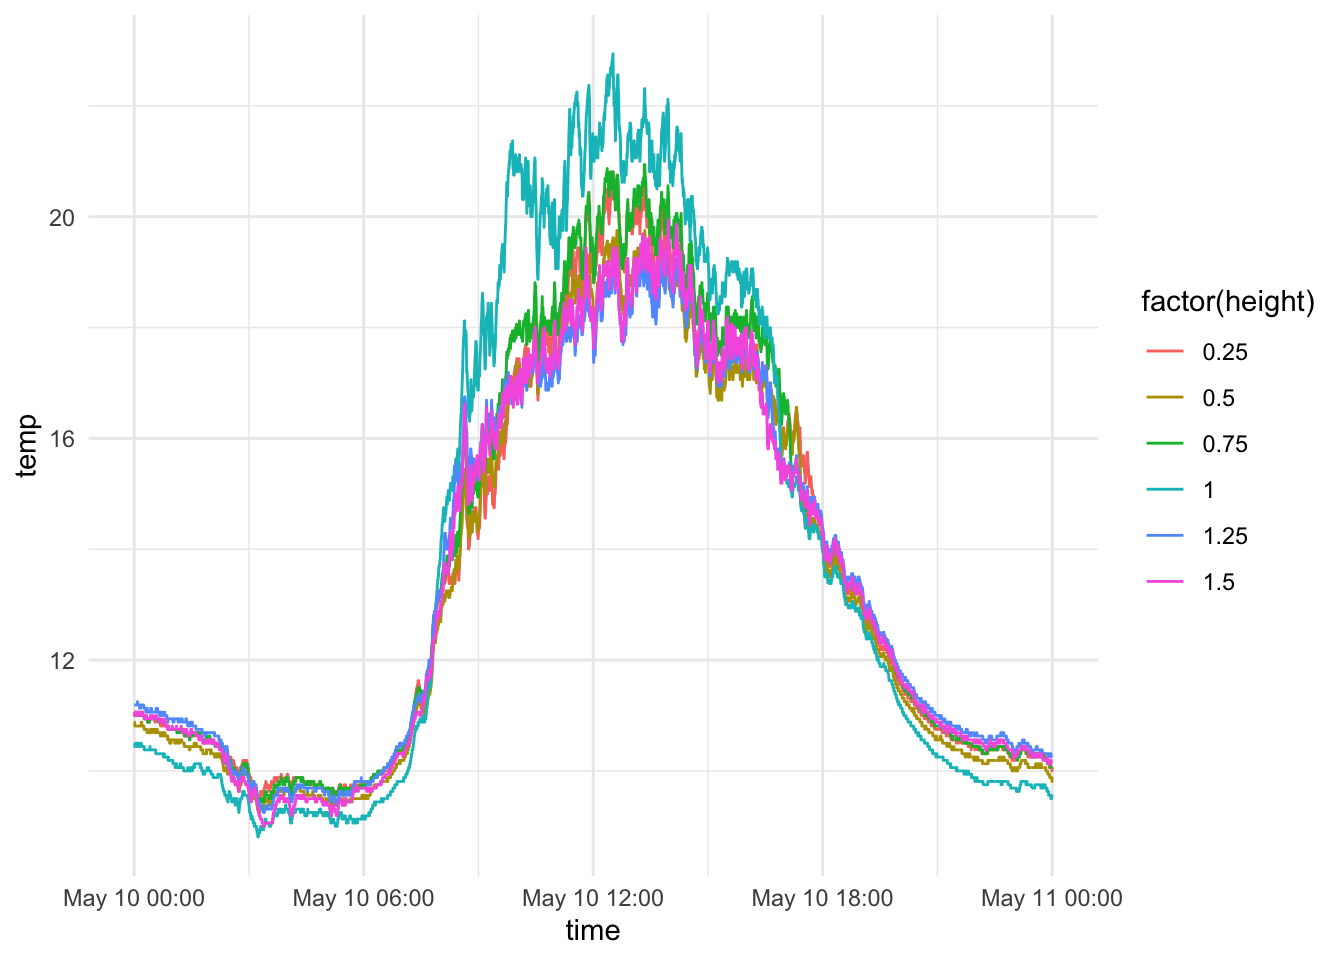
\includegraphics{Research_book_files/figure-latex/unnamed-chunk-18-1.pdf}

\begin{Shaded}
\begin{Highlighting}[]
\CommentTok{#ggplotly()}
\end{Highlighting}
\end{Shaded}

Add heights (Roghly .25 m apart)

\begin{Shaded}
\begin{Highlighting}[]
\NormalTok{mclim_}\DecValTok{2018}\OperatorTok{$}\NormalTok{height <-}\StringTok{ }\DecValTok{0}

\NormalTok{mclim_}\DecValTok{2018}\NormalTok{[mclim_}\DecValTok{2018}\OperatorTok{$}\NormalTok{nodeid}\OperatorTok{==}\StringTok{'28FF80E24316043F'}\NormalTok{ ,]}\OperatorTok{$}\NormalTok{height <-}\StringTok{ }\FloatTok{0.25}
\NormalTok{mclim_}\DecValTok{2018}\NormalTok{[mclim_}\DecValTok{2018}\OperatorTok{$}\NormalTok{nodeid}\OperatorTok{==}\StringTok{'28FF7331441603A7'}\NormalTok{ ,]}\OperatorTok{$}\NormalTok{height <-}\StringTok{ }\FloatTok{0.5}
\NormalTok{mclim_}\DecValTok{2018}\NormalTok{[mclim_}\DecValTok{2018}\OperatorTok{$}\NormalTok{nodeid}\OperatorTok{==}\StringTok{'287F5B04000080C5'}\NormalTok{ ,]}\OperatorTok{$}\NormalTok{height <-}\StringTok{ }\FloatTok{0.75}
\NormalTok{mclim_}\DecValTok{2018}\NormalTok{[mclim_}\DecValTok{2018}\OperatorTok{$}\NormalTok{nodeid}\OperatorTok{==}\StringTok{'28FFB1C2501604A8'}\NormalTok{ ,]}\OperatorTok{$}\NormalTok{height <-}\StringTok{ }\DecValTok{1}
\NormalTok{mclim_}\DecValTok{2018}\NormalTok{[mclim_}\DecValTok{2018}\OperatorTok{$}\NormalTok{nodeid}\OperatorTok{==}\StringTok{'28CF6F0400008059'}\NormalTok{ ,]}\OperatorTok{$}\NormalTok{height <-}\FloatTok{1.25}
\NormalTok{mclim_}\DecValTok{2018}\NormalTok{[mclim_}\DecValTok{2018}\OperatorTok{$}\NormalTok{nodeid}\OperatorTok{==}\StringTok{'28FF5B69501604F2'}\NormalTok{ ,]}\OperatorTok{$}\NormalTok{height <-}\StringTok{ }\FloatTok{1.5}
\end{Highlighting}
\end{Shaded}

Basic plot (May 10th) - By height

\begin{Shaded}
\begin{Highlighting}[]
\NormalTok{## 5-21-2018}
\NormalTok{mclim_}\DecValTok{2018} \OperatorTok\StringTok{ }\KeywordTok{filter}\NormalTok{(}\KeywordTok{day}\NormalTok{(time) }\OperatorTok\StringTok{ '10'}\NormalTok{) }\OperatorTok
\KeywordTok{ggplot}\NormalTok{( }\KeywordTok{aes}\NormalTok{(time,temp,}\DataTypeTok{color =} \KeywordTok{factor}\NormalTok{(height))) }\OperatorTok{+}\StringTok{ }\KeywordTok{geom_line}\NormalTok{() }\OperatorTok{+}\StringTok{ }\KeywordTok{theme_minimal}\NormalTok{()}
\end{Highlighting}
\end{Shaded}

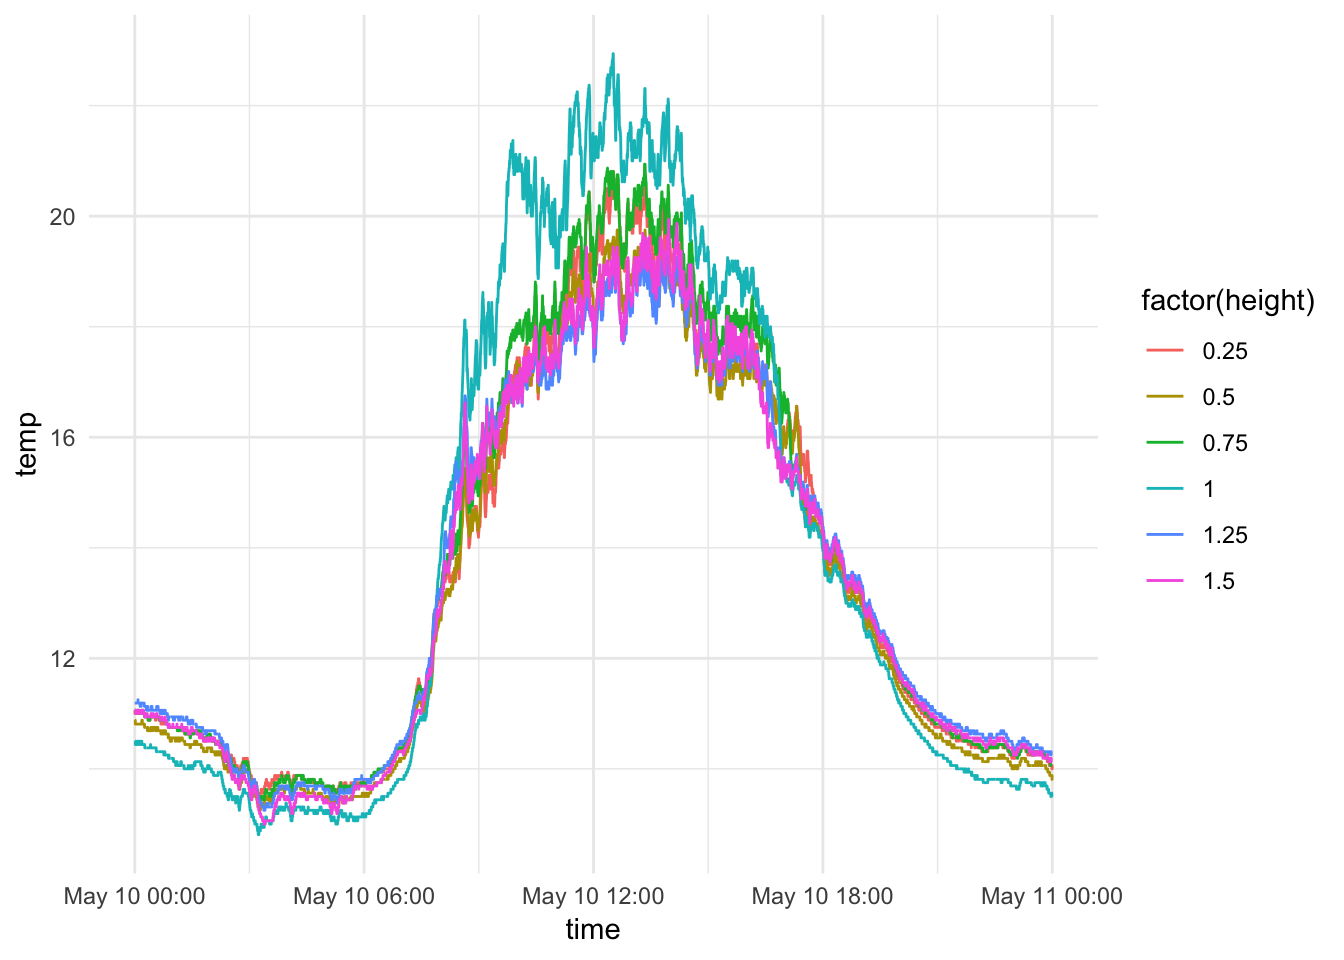
\includegraphics{Research_book_files/figure-latex/unnamed-chunk-20-1.pdf}

\begin{Shaded}
\begin{Highlighting}[]
\CommentTok{#ggplotly()}
\end{Highlighting}
\end{Shaded}

Add simulated wind profile

\begin{Shaded}
\begin{Highlighting}[]
\NormalTok{mclim_}\DecValTok{2018}\OperatorTok{$}\NormalTok{ws <-}\StringTok{ }\DecValTok{0}
\NormalTok{mclim_}\DecValTok{2018}\NormalTok{[mclim_}\DecValTok{2018}\OperatorTok{$}\NormalTok{nodeid}\OperatorTok{==}\StringTok{'287F5B04000080C5'}\NormalTok{,]}\OperatorTok{$}\NormalTok{ws <-}\StringTok{ }\FloatTok{4.34}
\NormalTok{mclim_}\DecValTok{2018}\NormalTok{[mclim_}\DecValTok{2018}\OperatorTok{$}\NormalTok{nodeid}\OperatorTok{==}\StringTok{'28FF80E24316043F'}\NormalTok{ ,]}\OperatorTok{$}\NormalTok{ws <-}\StringTok{ }\FloatTok{2.02}
\NormalTok{mclim_}\DecValTok{2018}\NormalTok{[mclim_}\DecValTok{2018}\OperatorTok{$}\NormalTok{nodeid}\OperatorTok{==}\StringTok{'28FFB1C2501604A8'}\NormalTok{ ,]}\OperatorTok{$}\NormalTok{ws <-}\StringTok{ }\FloatTok{5.20}
\NormalTok{mclim_}\DecValTok{2018}\NormalTok{[mclim_}\DecValTok{2018}\OperatorTok{$}\NormalTok{nodeid}\OperatorTok{==}\StringTok{'28FF7331441603A7'}\NormalTok{ ,]}\OperatorTok{$}\NormalTok{ws <-}\StringTok{ }\FloatTok{3.45}
\NormalTok{mclim_}\DecValTok{2018}\NormalTok{[mclim_}\DecValTok{2018}\OperatorTok{$}\NormalTok{nodeid}\OperatorTok{==}\StringTok{'28FF5B69501604F2'}\NormalTok{ ,]}\OperatorTok{$}\NormalTok{ws <-}\StringTok{ }\FloatTok{7.56}
\NormalTok{mclim_}\DecValTok{2018}\NormalTok{[mclim_}\DecValTok{2018}\OperatorTok{$}\NormalTok{nodeid}\OperatorTok{==}\StringTok{'28CF6F0400008059'}\NormalTok{ ,]}\OperatorTok{$}\NormalTok{ws <-}\FloatTok{6.54}
\end{Highlighting}
\end{Shaded}

Redo the plot by height

\begin{Shaded}
\begin{Highlighting}[]
\NormalTok{## 5-21-2018}
\NormalTok{mclim_}\DecValTok{2018} \OperatorTok\StringTok{ }\KeywordTok{filter}\NormalTok{(}\KeywordTok{day}\NormalTok{(time) }\OperatorTok\StringTok{ '10'}\NormalTok{, height }\OperatorTok\StringTok{ }\KeywordTok{c}\NormalTok{(}\FloatTok{0.25}\NormalTok{,}\DecValTok{1}\NormalTok{)) }\OperatorTok
\KeywordTok{ggplot}\NormalTok{( }\KeywordTok{aes}\NormalTok{(time,temp,}\DataTypeTok{color =} \KeywordTok{factor}\NormalTok{(height))) }\OperatorTok{+}\StringTok{ }\KeywordTok{geom_line}\NormalTok{() }\OperatorTok{+}\StringTok{ }\KeywordTok{theme_minimal}\NormalTok{()}
\end{Highlighting}
\end{Shaded}

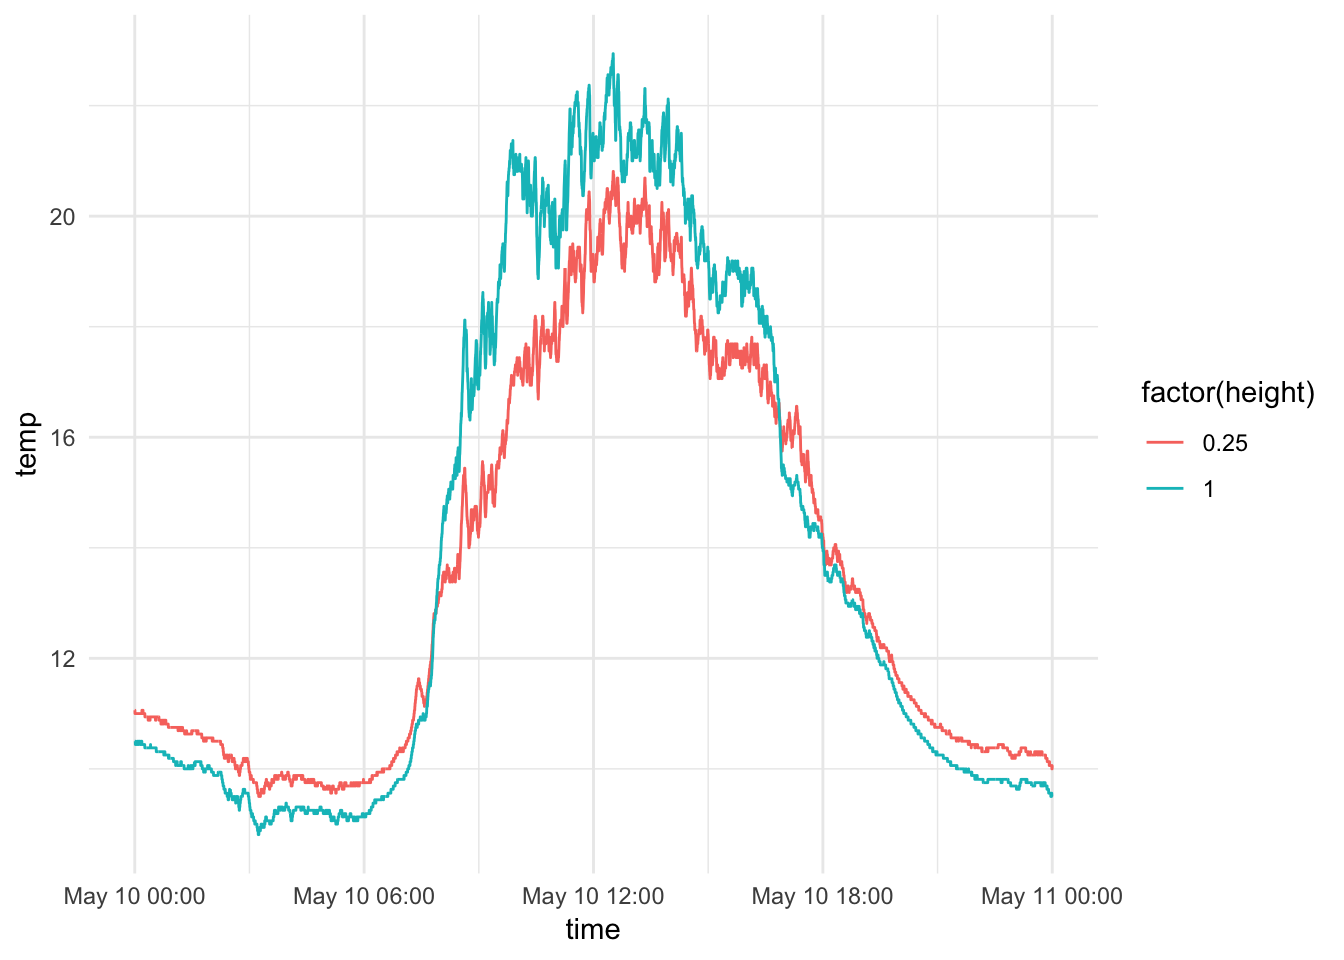
\includegraphics{Research_book_files/figure-latex/unnamed-chunk-22-1.pdf}

Redo the plot by height for Wind Speed

\begin{Shaded}
\begin{Highlighting}[]
\NormalTok{## 5-21-2018}
\NormalTok{mclim_}\DecValTok{2018} \OperatorTok\StringTok{ }\KeywordTok{filter}\NormalTok{(}\KeywordTok{day}\NormalTok{(time) }\OperatorTok\StringTok{ '10'}\NormalTok{, height }\OperatorTok\StringTok{ }\KeywordTok{c}\NormalTok{(}\FloatTok{0.25}\NormalTok{,}\FloatTok{0.5}\NormalTok{,}\FloatTok{0.75}\NormalTok{,}\DecValTok{1}\NormalTok{)) }\OperatorTok
\KeywordTok{ggplot}\NormalTok{( }\KeywordTok{aes}\NormalTok{(time,ws,}\DataTypeTok{color =} \KeywordTok{factor}\NormalTok{(height))) }\OperatorTok{+}\StringTok{ }\KeywordTok{geom_line}\NormalTok{() }\OperatorTok{+}\StringTok{ }\KeywordTok{theme_minimal}\NormalTok{()}
\end{Highlighting}
\end{Shaded}

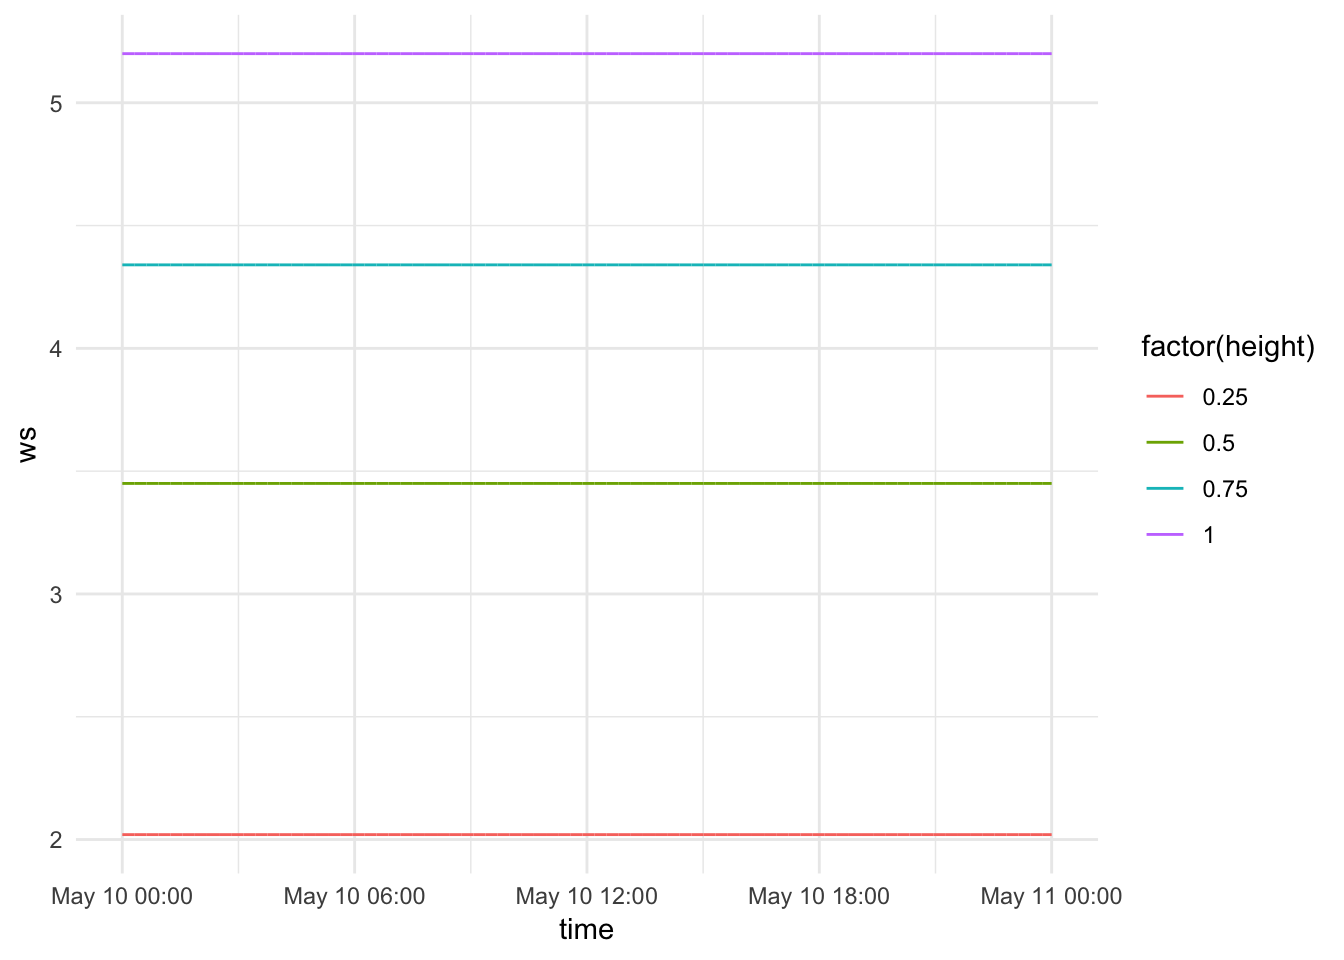
\includegraphics{Research_book_files/figure-latex/unnamed-chunk-23-1.pdf}

Calculate (Wind speed at any height = U\_star/K*log(Z/Z0))

Calculate zero plane displcement

\begin{Shaded}
\begin{Highlighting}[]
\CommentTok{#TODO - Do by each hour}
\NormalTok{zeroDM<-}\StringTok{ }\KeywordTok{lm}\NormalTok{(}\KeywordTok{log}\NormalTok{(mclim_}\DecValTok{2018}\OperatorTok{$}\NormalTok{height) }\OperatorTok{~}\StringTok{ }\NormalTok{mclim_}\DecValTok{2018}\OperatorTok{$}\NormalTok{ws)}
\NormalTok{zD <-}\StringTok{ }\KeywordTok{exp}\NormalTok{(zeroDM}\OperatorTok{$}\NormalTok{coeff[}\DecValTok{1}\NormalTok{])}
\CommentTok{#.16}
\end{Highlighting}
\end{Shaded}

Calculate roughness and Z*

\begin{Shaded}
\begin{Highlighting}[]
\CommentTok{#With zero plane dispacement}
\NormalTok{sRM<-}\StringTok{ }\KeywordTok{lm}\NormalTok{(mclim_}\DecValTok{2018}\OperatorTok{$}\NormalTok{ws }\OperatorTok{~}\StringTok{ }\KeywordTok{log}\NormalTok{(mclim_}\DecValTok{2018}\OperatorTok{$}\NormalTok{height}\OperatorTok{-}\NormalTok{zD))}

\NormalTok{srIntercept <-}\StringTok{ }\NormalTok{sRM}\OperatorTok{$}\NormalTok{coeff[}\DecValTok{1}\NormalTok{]}
\NormalTok{srSlope <-}\StringTok{ }\NormalTok{sRM}\OperatorTok{$}\NormalTok{coeff[}\DecValTok{2}\NormalTok{]}

\NormalTok{K=}\FloatTok{0.4} \CommentTok{# Von Karman constant}

\NormalTok{z0<-}\StringTok{  }\KeywordTok{exp}\NormalTok{(}\OperatorTok{-}\NormalTok{srIntercept}\OperatorTok{/}\NormalTok{srSlope) }\CommentTok{#0.04}
\NormalTok{U_star<-}\StringTok{  }\NormalTok{srSlope}\OperatorTok{*}\NormalTok{K}
\end{Highlighting}
\end{Shaded}

Repeat this for each site \#\# 7-21-2018

\begin{Shaded}
\begin{Highlighting}[]
\CommentTok{#With zero plane dispacement}
\KeywordTok{library}\NormalTok{(rgdal) }\CommentTok{#this package is necessary to import the .asc file in R.}
\KeywordTok{library}\NormalTok{(rasterVis) }\CommentTok{#this package has the function which allows the 3D plotting.}

\CommentTok{#set the path where the file is, and import it into R.}
\NormalTok{r=}\StringTok{ }\KeywordTok{raster}\NormalTok{(}\KeywordTok{paste}\NormalTok{(}\StringTok{"./data/rainier_2012_dtm_5_hs.tif"}\NormalTok{, }\DataTypeTok{sep=}\StringTok{""}\NormalTok{))}

\CommentTok{#visualize the raster in 3D}
\KeywordTok{plot}\NormalTok{(r,}\DataTypeTok{lit=}\OtherTok{TRUE}\NormalTok{)}
\end{Highlighting}
\end{Shaded}

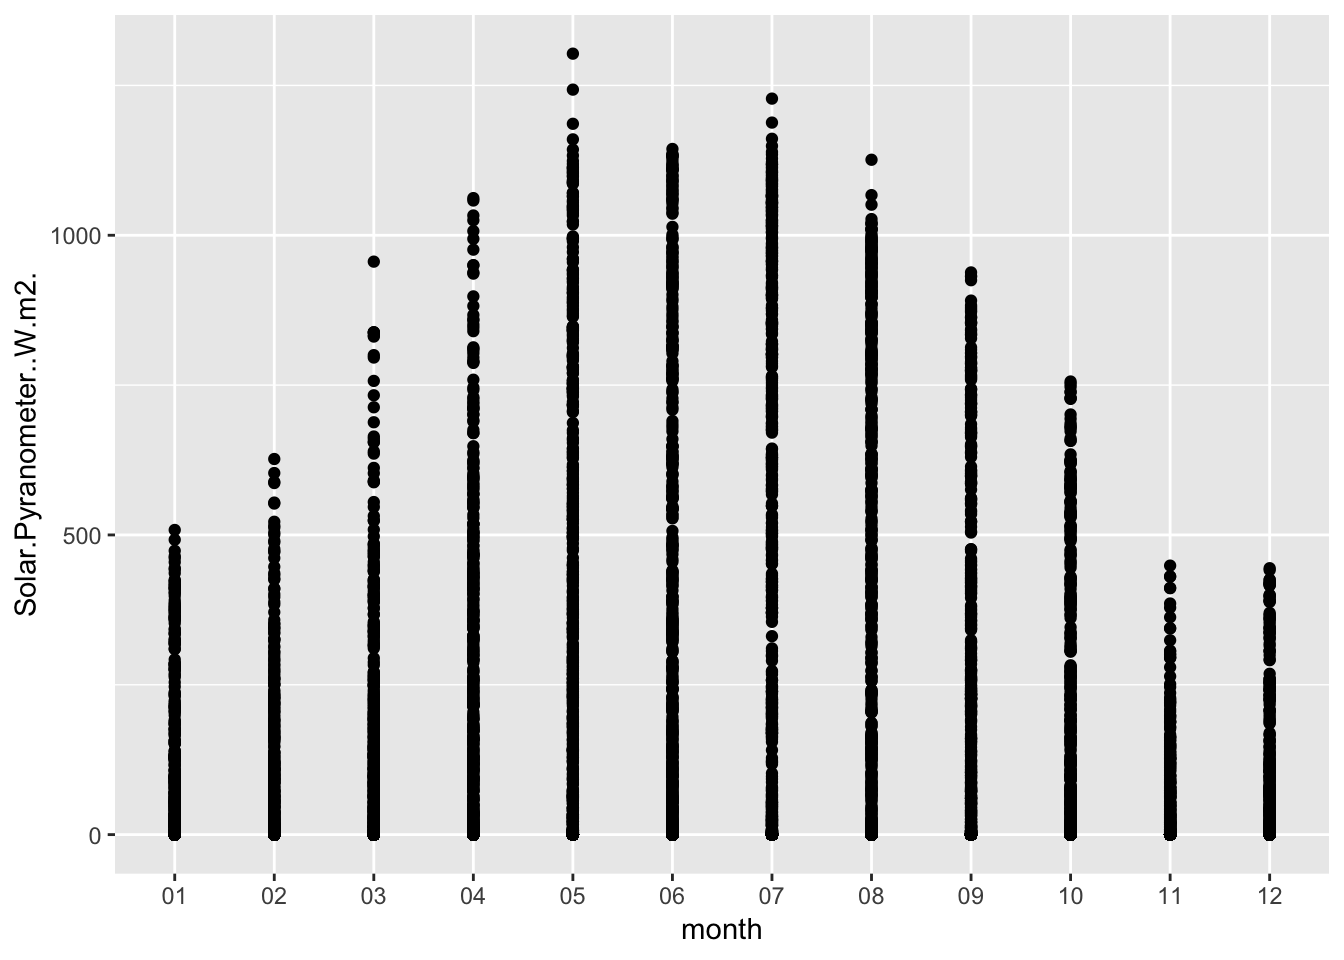
\includegraphics{Research_book_files/figure-latex/unnamed-chunk-26-1.pdf}

\begin{Shaded}
\begin{Highlighting}[]
\KeywordTok{library}\NormalTok{(tidyverse)}
\NormalTok{fs <-}\StringTok{ }\KeywordTok{list.files}\NormalTok{(}\DataTypeTok{path=}\StringTok{"./data"}\NormalTok{, }\DataTypeTok{pattern =} \StringTok{"rainier*"}\NormalTok{, }\DataTypeTok{full.names =} \OtherTok{TRUE}\NormalTok{)}

\NormalTok{r1 <-}\StringTok{ }\KeywordTok{raster}\NormalTok{(fs[}\DecValTok{1}\NormalTok{])}
\NormalTok{r1[] <-}\StringTok{ }\DecValTok{1}\OperatorTok{:}\KeywordTok{ncell}\NormalTok{(r1)}
\NormalTok{r2 <-}\StringTok{ }\KeywordTok{raster}\NormalTok{(fs[}\DecValTok{2}\NormalTok{])}
\NormalTok{r3 <-}\StringTok{ }\KeywordTok{raster}\NormalTok{(fs[}\DecValTok{3}\NormalTok{])}
\NormalTok{r4 <-}\StringTok{ }\KeywordTok{raster}\NormalTok{(fs[}\DecValTok{4}\NormalTok{])}
\KeywordTok{res}\NormalTok{(r2) <-}\StringTok{ }\KeywordTok{c}\NormalTok{(}\KeywordTok{xres}\NormalTok{(r1), }\KeywordTok{yres}\NormalTok{(r1))}
\NormalTok{r2[] <-}\StringTok{ }\DecValTok{1}\OperatorTok{:}\KeywordTok{ncell}\NormalTok{(r2)}
\NormalTok{r3[] <-}\StringTok{ }\DecValTok{1}\OperatorTok{:}\KeywordTok{ncell}\NormalTok{(r3)}
\NormalTok{r4[] <-}\StringTok{ }\DecValTok{1}\OperatorTok{:}\KeywordTok{ncell}\NormalTok{(r4)}

\NormalTok{x <-}\StringTok{ }\KeywordTok{list}\NormalTok{(r1, r2,r3,r4)}
\NormalTok{x}\OperatorTok{$}\NormalTok{filename <-}\StringTok{ 'test.tif'}
\NormalTok{x}\OperatorTok{$}\NormalTok{overwrite <-}\StringTok{ }\OtherTok{TRUE}
\NormalTok{m <-}\StringTok{ }\KeywordTok{do.call}\NormalTok{(merge, x)}
\end{Highlighting}
\end{Shaded}

\section{7-25-2018}\label{section-6}

Check the diurnal variation for summer, using Paradise as a proxy

\begin{Shaded}
\begin{Highlighting}[]
\NormalTok{Paradise_}\DecValTok{2017} \OperatorTok\StringTok{ }\KeywordTok{group_by}\NormalTok{(date,month,hr) }\OperatorTok\StringTok{ }\KeywordTok{ggplot}\NormalTok{(}\KeywordTok{aes}\NormalTok{(month,Solar.Pyranometer..W.m2.)) }\OperatorTok{+}\StringTok{ }\KeywordTok{geom_point}\NormalTok{() }
\end{Highlighting}
\end{Shaded}

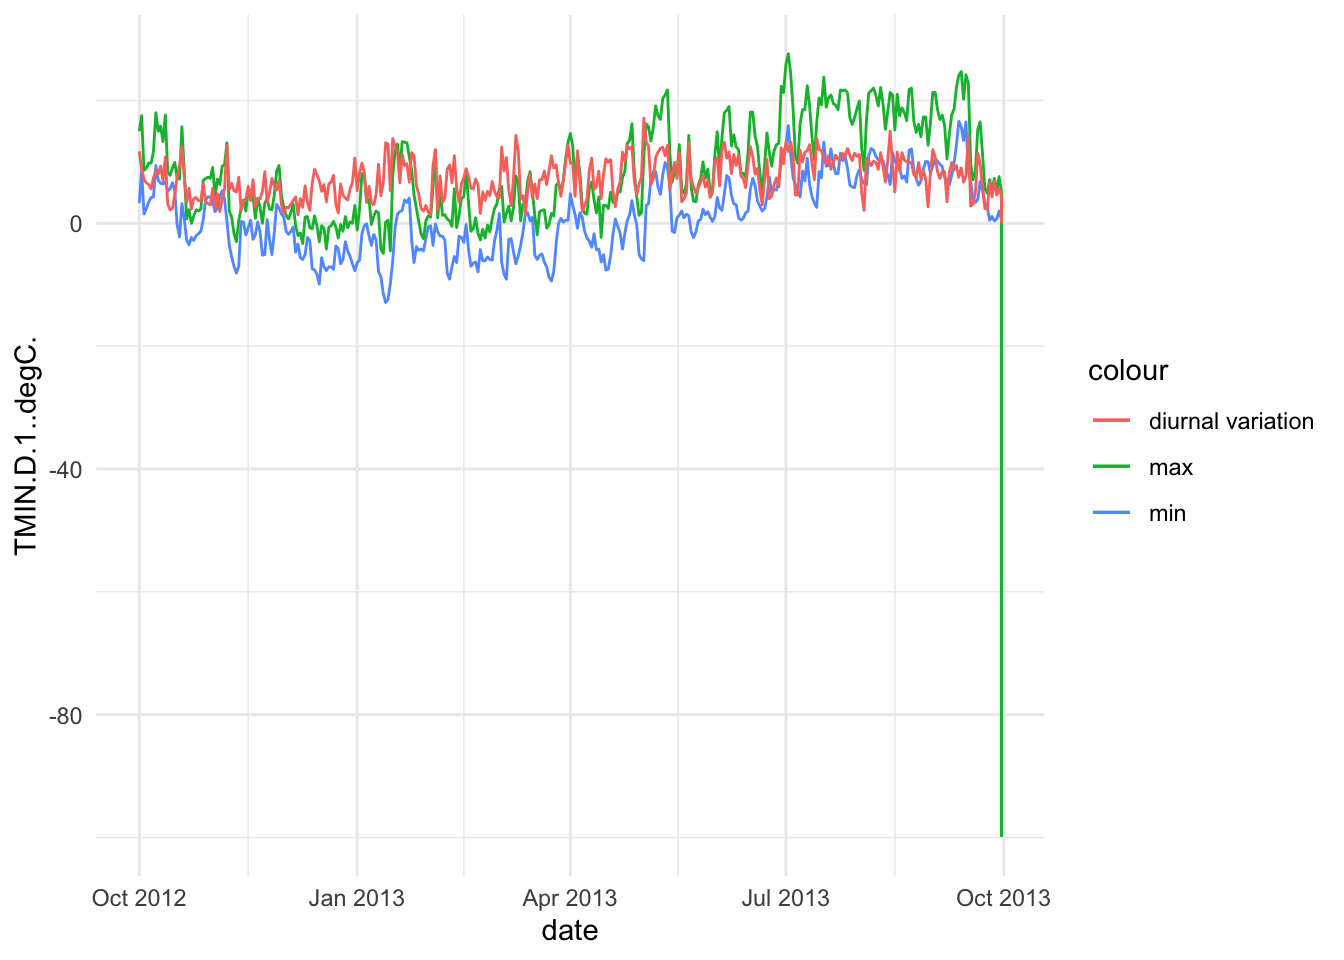
\includegraphics{Research_book_files/figure-latex/unnamed-chunk-27-1.pdf}

\begin{Shaded}
\begin{Highlighting}[]
\CommentTok{#.16}
\end{Highlighting}
\end{Shaded}

Use SNOTEL data from Paradise(Latitude: 46.78 Longitude: -121.74)

Check the diurnal variation for summer, using Paradise as a proxy

\begin{Shaded}
\begin{Highlighting}[]
\NormalTok{Paradise_Snotel_}\DecValTok{2013}\NormalTok{<-}\StringTok{ }\KeywordTok{read.csv}\NormalTok{(}\StringTok{'./data/679_STAND_WATERYEAR=2013.csv'}\NormalTok{)}
\NormalTok{Paradise_Snotel_}\DecValTok{2013}\OperatorTok{$}\NormalTok{date <-}\StringTok{ }\KeywordTok{as.Date}\NormalTok{(Paradise_Snotel_}\DecValTok{2013}\OperatorTok{$}\NormalTok{Date, }\StringTok{"%Y-%m-%d"}\NormalTok{)}
\NormalTok{Paradise_Snotel_}\DecValTok{2013}\OperatorTok{$}\NormalTok{month <-}\StringTok{ }\KeywordTok{strftime}\NormalTok{(Paradise_Snotel_}\DecValTok{2013}\OperatorTok{$}\NormalTok{Date,}\StringTok{'%m'}\NormalTok{)}

\NormalTok{Paradise_Snotel_}\DecValTok{2012}\NormalTok{<-}\StringTok{ }\KeywordTok{read.csv}\NormalTok{(}\StringTok{'./data/679_STAND_WATERYEAR=2012.csv'}\NormalTok{)}
\NormalTok{Paradise_Snotel_}\DecValTok{2012}\OperatorTok{$}\NormalTok{date <-}\StringTok{ }\KeywordTok{as.Date}\NormalTok{(Paradise_Snotel_}\DecValTok{2012}\OperatorTok{$}\NormalTok{Date, }\StringTok{"%Y-%m-%d"}\NormalTok{)}
\NormalTok{Paradise_Snotel_}\DecValTok{2012}\OperatorTok{$}\NormalTok{month <-}\StringTok{ }\KeywordTok{strftime}\NormalTok{(Paradise_Snotel_}\DecValTok{2012}\OperatorTok{$}\NormalTok{Date,}\StringTok{'%m'}\NormalTok{)}

\NormalTok{Paradise_Snotel_}\DecValTok{2011}\NormalTok{<-}\StringTok{ }\KeywordTok{read.csv}\NormalTok{(}\StringTok{'./data/679_STAND_WATERYEAR=2011.csv'}\NormalTok{)}
\NormalTok{Paradise_Snotel_}\DecValTok{2011}\OperatorTok{$}\NormalTok{date <-}\StringTok{ }\KeywordTok{as.Date}\NormalTok{(Paradise_Snotel_}\DecValTok{2011}\OperatorTok{$}\NormalTok{Date, }\StringTok{"%Y-%m-%d"}\NormalTok{)}
\NormalTok{Paradise_Snotel_}\DecValTok{2011}\OperatorTok{$}\NormalTok{month <-}\StringTok{ }\KeywordTok{strftime}\NormalTok{(Paradise_Snotel_}\DecValTok{2011}\OperatorTok{$}\NormalTok{Date,}\StringTok{'%m'}\NormalTok{)}

\NormalTok{Paradise_Snotel_}\DecValTok{2013} \OperatorTok\StringTok{ }\KeywordTok{group_by}\NormalTok{(date,month) }\OperatorTok\StringTok{ }\KeywordTok{mutate}\NormalTok{(}\DataTypeTok{diva=}\NormalTok{TMAX.D.}\DecValTok{1}\NormalTok{..degC.}\OperatorTok{-}\NormalTok{TMIN.D.}\DecValTok{1}\NormalTok{..degC.)}\OperatorTok\StringTok{ }\KeywordTok{ggplot}\NormalTok{() }\OperatorTok{+}\StringTok{ }\KeywordTok{geom_line}\NormalTok{(}\KeywordTok{aes}\NormalTok{(date,TMIN.D.}\DecValTok{1}\NormalTok{..degC.,}\DataTypeTok{colour=}\StringTok{'min'}\NormalTok{))  }\OperatorTok{+}\KeywordTok{geom_line}\NormalTok{(}\KeywordTok{aes}\NormalTok{(date,TMAX.D.}\DecValTok{1}\NormalTok{..degC.,}\DataTypeTok{colour=}\StringTok{'max'}\NormalTok{)) }\OperatorTok{+}\KeywordTok{geom_line}\NormalTok{(}\KeywordTok{aes}\NormalTok{(date,diva,}\DataTypeTok{colour=}\StringTok{'diurnal variation'}\NormalTok{))}\OperatorTok{+}\StringTok{ }\KeywordTok{theme_minimal}\NormalTok{()}
\end{Highlighting}
\end{Shaded}

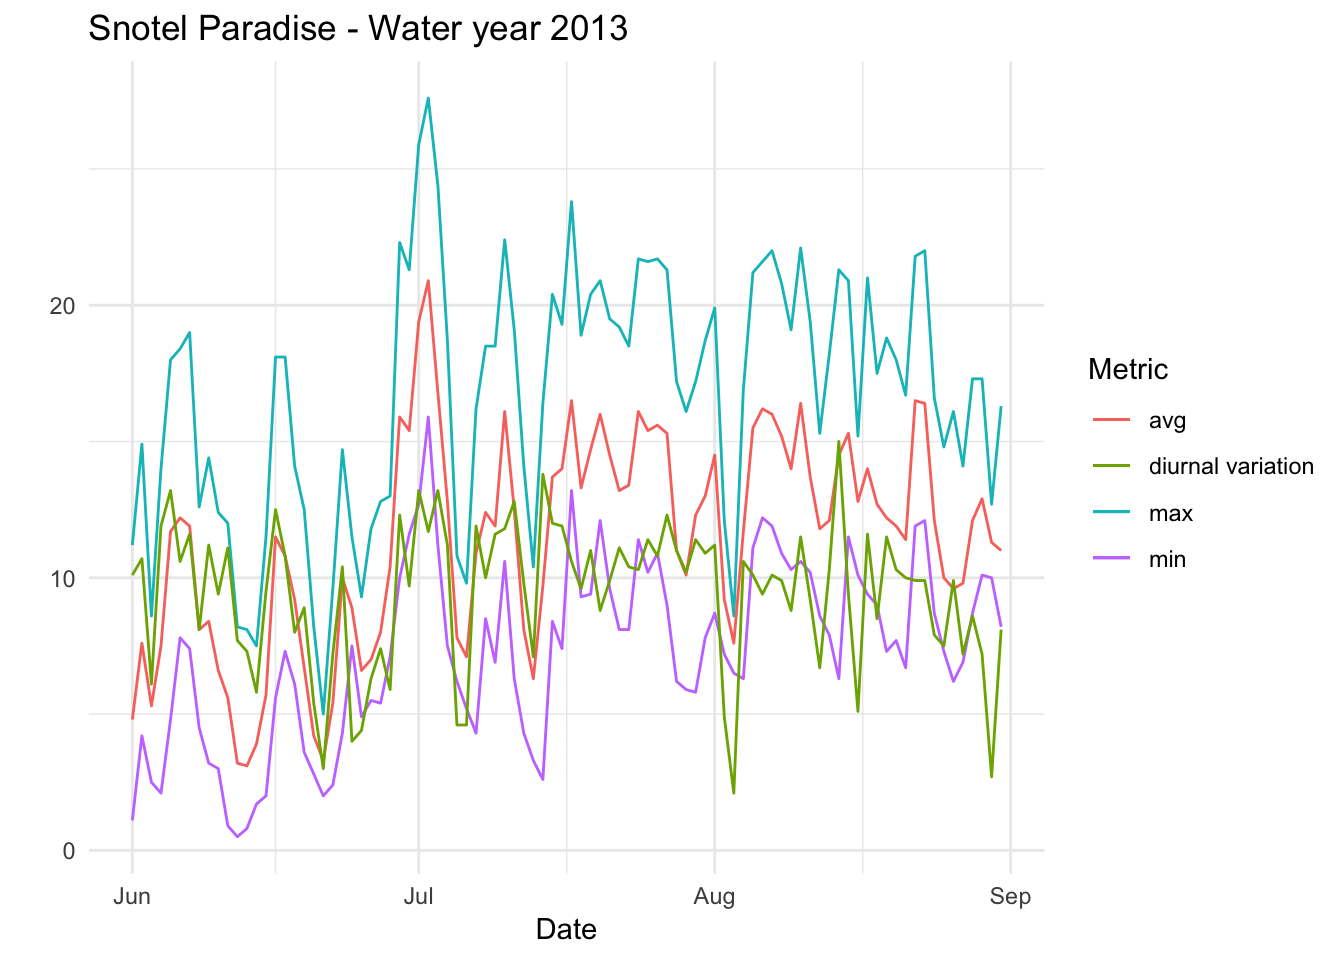
\includegraphics{Research_book_files/figure-latex/unnamed-chunk-28-1.pdf}

\begin{Shaded}
\begin{Highlighting}[]
\CommentTok{#.16}
\end{Highlighting}
\end{Shaded}

Only Summer

\begin{Shaded}
\begin{Highlighting}[]
\NormalTok{Paradise_Snotel_}\DecValTok{2013} \OperatorTok\StringTok{ }\KeywordTok{group_by}\NormalTok{(date,month) }\OperatorTok\StringTok{ }\KeywordTok{filter}\NormalTok{(}\KeywordTok{as.numeric}\NormalTok{(month) }\OperatorTok\StringTok{ }\KeywordTok{c}\NormalTok{(}\DecValTok{6}\NormalTok{,}\DecValTok{7}\NormalTok{,}\DecValTok{8}\NormalTok{)) }\OperatorTok\StringTok{ }\KeywordTok{mutate}\NormalTok{(}\DataTypeTok{diva=}\NormalTok{TMAX.D.}\DecValTok{1}\NormalTok{..degC.}\OperatorTok{-}\NormalTok{TMIN.D.}\DecValTok{1}\NormalTok{..degC.)}\OperatorTok\StringTok{ }\KeywordTok{ggplot}\NormalTok{() }\OperatorTok{+}\StringTok{ }\KeywordTok{geom_line}\NormalTok{(}\KeywordTok{aes}\NormalTok{(date,TMIN.D.}\DecValTok{1}\NormalTok{..degC.,}\DataTypeTok{colour=}\StringTok{'min'}\NormalTok{))  }\OperatorTok{+}\KeywordTok{geom_line}\NormalTok{(}\KeywordTok{aes}\NormalTok{(date,TMAX.D.}\DecValTok{1}\NormalTok{..degC.,}\DataTypeTok{colour=}\StringTok{'max'}\NormalTok{))}\OperatorTok{+}\KeywordTok{geom_line}\NormalTok{(}\KeywordTok{aes}\NormalTok{(date,TAVG.D.}\DecValTok{1}\NormalTok{..degC.,}\DataTypeTok{colour=}\StringTok{'avg'}\NormalTok{)) }\OperatorTok{+}\KeywordTok{geom_line}\NormalTok{(}\KeywordTok{aes}\NormalTok{(date,diva,}\DataTypeTok{colour=}\StringTok{'diurnal variation'}\NormalTok{))}\OperatorTok{+}\StringTok{ }\KeywordTok{theme_minimal}\NormalTok{() }\OperatorTok{+}\KeywordTok{xlab}\NormalTok{(}\StringTok{"Date"}\NormalTok{) }\OperatorTok{+}\StringTok{ }\KeywordTok{ylab}\NormalTok{(}\StringTok{""}\NormalTok{) }\OperatorTok{+}\StringTok{ }\KeywordTok{ggtitle}\NormalTok{(}\StringTok{"Snotel Paradise - Water year 2013 "}\NormalTok{) }\OperatorTok{+}\StringTok{ }\KeywordTok{scale_color_discrete}\NormalTok{(}\DataTypeTok{name=}\StringTok{"Metric"}\NormalTok{)}
\end{Highlighting}
\end{Shaded}

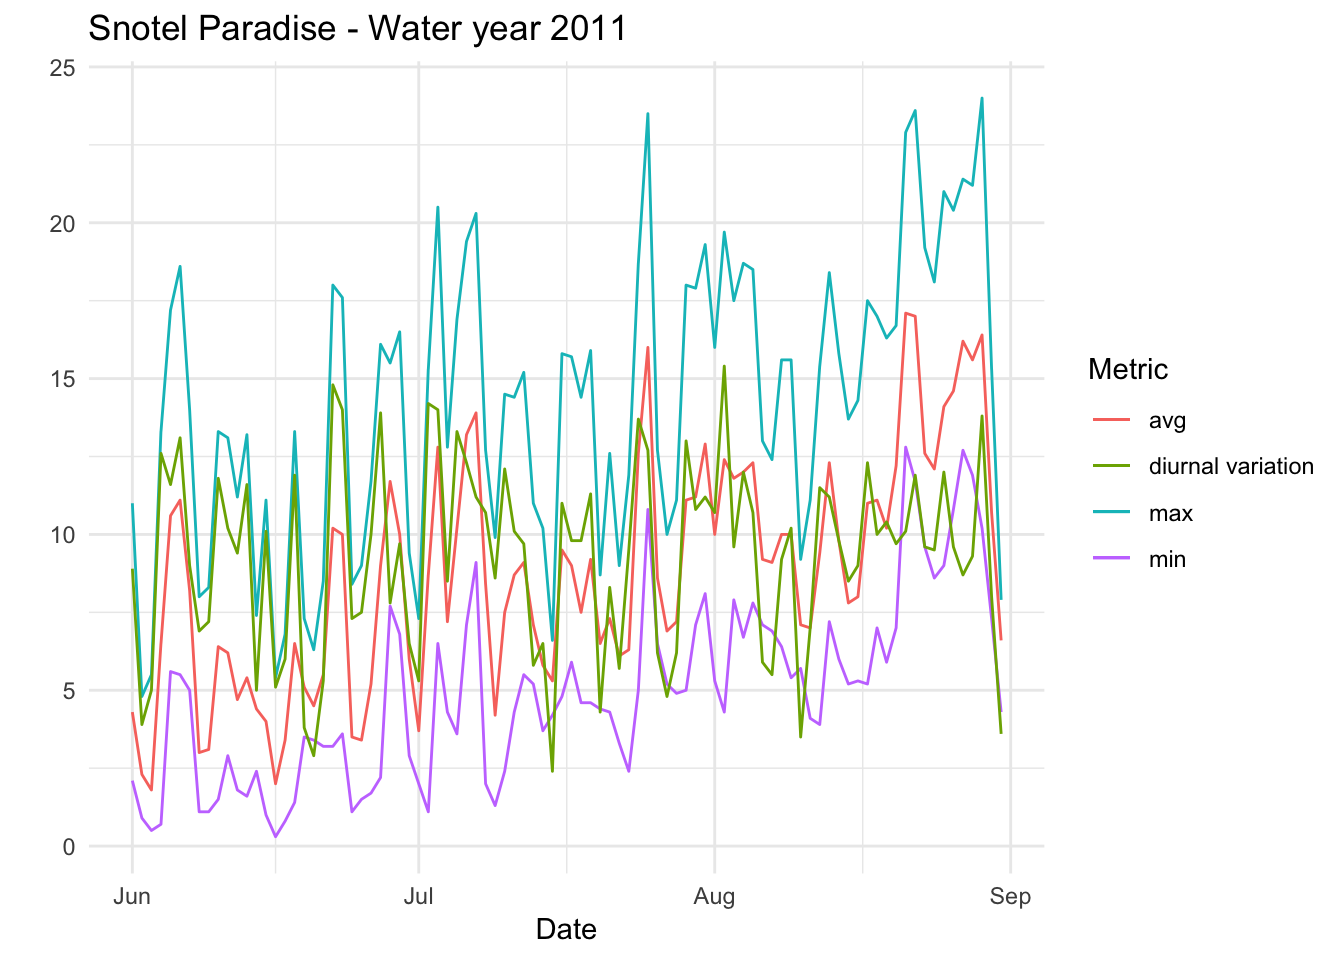
\includegraphics{Research_book_files/figure-latex/unnamed-chunk-29-1.pdf}

\begin{Shaded}
\begin{Highlighting}[]
\CommentTok{#.16}
\end{Highlighting}
\end{Shaded}

For 2012

\begin{Shaded}
\begin{Highlighting}[]
\NormalTok{Paradise_Snotel_}\DecValTok{2012} \OperatorTok\StringTok{ }\KeywordTok{group_by}\NormalTok{(date,month) }\OperatorTok\StringTok{ }\KeywordTok{filter}\NormalTok{(}\KeywordTok{as.numeric}\NormalTok{(month) }\OperatorTok\StringTok{ }\KeywordTok{c}\NormalTok{(}\DecValTok{6}\NormalTok{,}\DecValTok{7}\NormalTok{,}\DecValTok{8}\NormalTok{) }\OperatorTok{&}\StringTok{ }\NormalTok{TMIN.D.}\DecValTok{1}\NormalTok{..degC. }\OperatorTok{!=}\StringTok{ }\OperatorTok{-}\FloatTok{99.9}\NormalTok{) }\OperatorTok\StringTok{ }\KeywordTok{mutate}\NormalTok{(}\DataTypeTok{diva=}\NormalTok{TMAX.D.}\DecValTok{1}\NormalTok{..degC.}\OperatorTok{-}\NormalTok{TMIN.D.}\DecValTok{1}\NormalTok{..degC.)}\OperatorTok\StringTok{ }\KeywordTok{ggplot}\NormalTok{() }\OperatorTok{+}\StringTok{ }\KeywordTok{geom_line}\NormalTok{(}\KeywordTok{aes}\NormalTok{(date,TMIN.D.}\DecValTok{1}\NormalTok{..degC.,}\DataTypeTok{colour=}\StringTok{'min'}\NormalTok{))  }\OperatorTok{+}\KeywordTok{geom_line}\NormalTok{(}\KeywordTok{aes}\NormalTok{(date,TMAX.D.}\DecValTok{1}\NormalTok{..degC.,}\DataTypeTok{colour=}\StringTok{'max'}\NormalTok{))}\OperatorTok{+}\KeywordTok{geom_line}\NormalTok{(}\KeywordTok{aes}\NormalTok{(date,TAVG.D.}\DecValTok{1}\NormalTok{..degC.,}\DataTypeTok{colour=}\StringTok{'avg'}\NormalTok{)) }\OperatorTok{+}\KeywordTok{geom_line}\NormalTok{(}\KeywordTok{aes}\NormalTok{(date,diva,}\DataTypeTok{colour=}\StringTok{'diurnal variation'}\NormalTok{))}\OperatorTok{+}\StringTok{ }\KeywordTok{theme_minimal}\NormalTok{() }\OperatorTok{+}\KeywordTok{xlab}\NormalTok{(}\StringTok{"Date"}\NormalTok{) }\OperatorTok{+}\StringTok{ }\KeywordTok{ylab}\NormalTok{(}\StringTok{""}\NormalTok{) }\OperatorTok{+}\StringTok{ }\KeywordTok{ggtitle}\NormalTok{(}\StringTok{"Snotel Paradise - Water year 2012 "}\NormalTok{) }\OperatorTok{+}\StringTok{ }\KeywordTok{scale_color_discrete}\NormalTok{(}\DataTypeTok{name=}\StringTok{"Metric"}\NormalTok{)}
\end{Highlighting}
\end{Shaded}

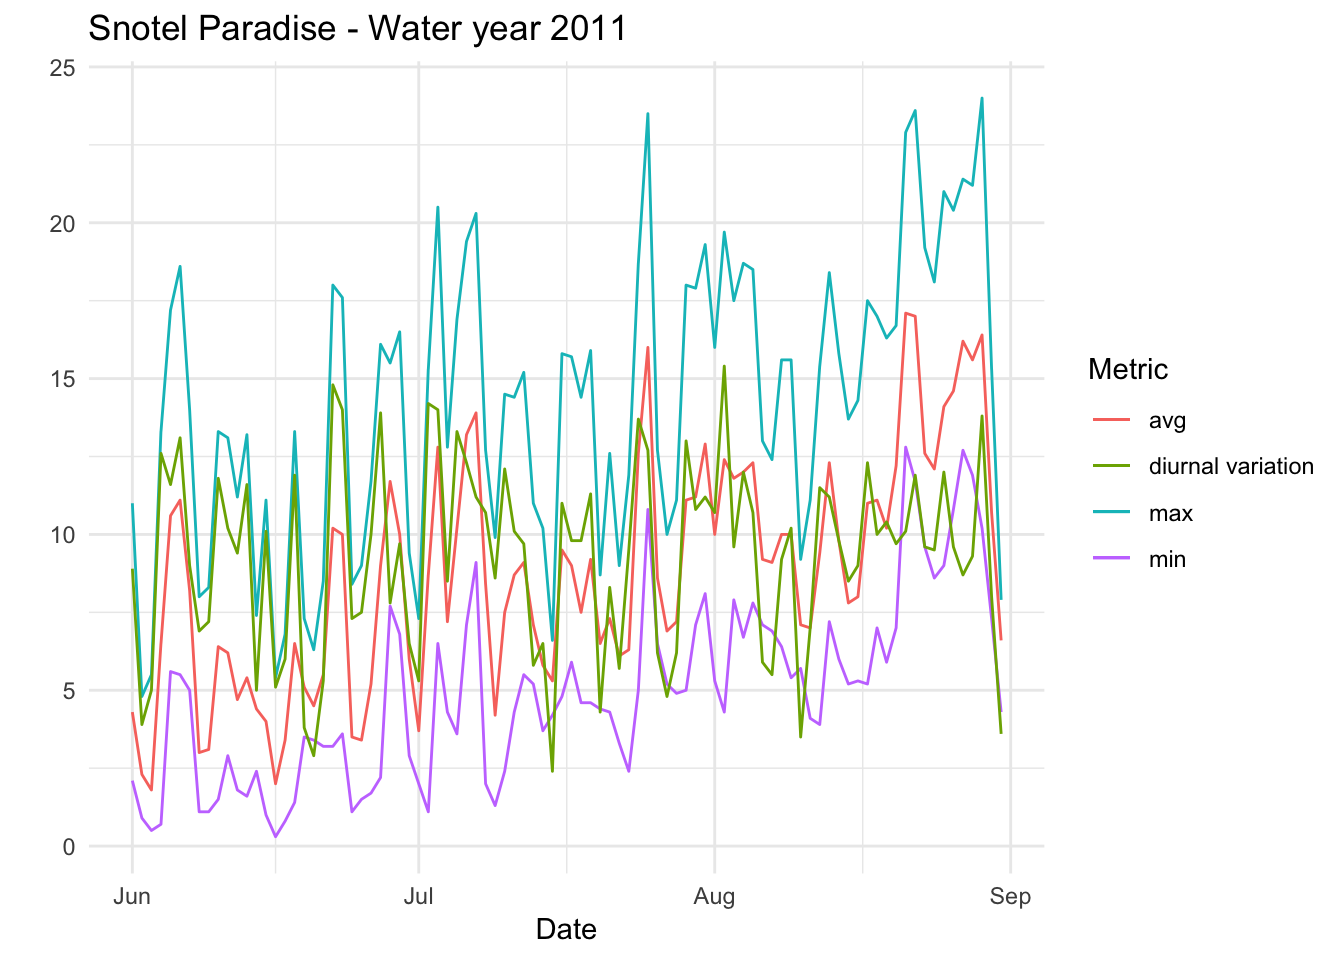
\includegraphics{Research_book_files/figure-latex/unnamed-chunk-30-1.pdf}

\begin{Shaded}
\begin{Highlighting}[]
\CommentTok{#.16}
\end{Highlighting}
\end{Shaded}

For 2011

\begin{Shaded}
\begin{Highlighting}[]
\NormalTok{Paradise_Snotel_}\DecValTok{2011} \OperatorTok\StringTok{ }\KeywordTok{group_by}\NormalTok{(date,month) }\OperatorTok\StringTok{ }\KeywordTok{filter}\NormalTok{(}\KeywordTok{as.numeric}\NormalTok{(month) }\OperatorTok\StringTok{ }\KeywordTok{c}\NormalTok{(}\DecValTok{6}\NormalTok{,}\DecValTok{7}\NormalTok{,}\DecValTok{8}\NormalTok{)) }\OperatorTok\StringTok{ }\KeywordTok{mutate}\NormalTok{(}\DataTypeTok{diva=}\NormalTok{TMAX.D.}\DecValTok{1}\NormalTok{..degC.}\OperatorTok{-}\NormalTok{TMIN.D.}\DecValTok{1}\NormalTok{..degC.)}\OperatorTok\StringTok{ }\KeywordTok{ggplot}\NormalTok{() }\OperatorTok{+}\StringTok{ }\KeywordTok{geom_line}\NormalTok{(}\KeywordTok{aes}\NormalTok{(date,TMIN.D.}\DecValTok{1}\NormalTok{..degC.,}\DataTypeTok{colour=}\StringTok{'min'}\NormalTok{))  }\OperatorTok{+}\KeywordTok{geom_line}\NormalTok{(}\KeywordTok{aes}\NormalTok{(date,TMAX.D.}\DecValTok{1}\NormalTok{..degC.,}\DataTypeTok{colour=}\StringTok{'max'}\NormalTok{))}\OperatorTok{+}\KeywordTok{geom_line}\NormalTok{(}\KeywordTok{aes}\NormalTok{(date,TAVG.D.}\DecValTok{1}\NormalTok{..degC.,}\DataTypeTok{colour=}\StringTok{'avg'}\NormalTok{)) }\OperatorTok{+}\KeywordTok{geom_line}\NormalTok{(}\KeywordTok{aes}\NormalTok{(date,diva,}\DataTypeTok{colour=}\StringTok{'diurnal variation'}\NormalTok{))}\OperatorTok{+}\StringTok{ }\KeywordTok{theme_minimal}\NormalTok{() }\OperatorTok{+}\KeywordTok{xlab}\NormalTok{(}\StringTok{"Date"}\NormalTok{) }\OperatorTok{+}\StringTok{ }\KeywordTok{ylab}\NormalTok{(}\StringTok{""}\NormalTok{) }\OperatorTok{+}\StringTok{ }\KeywordTok{ggtitle}\NormalTok{(}\StringTok{"Snotel Paradise - Water year 2011 "}\NormalTok{) }\OperatorTok{+}\StringTok{ }\KeywordTok{scale_color_discrete}\NormalTok{(}\DataTypeTok{name=}\StringTok{"Metric"}\NormalTok{)}
\end{Highlighting}
\end{Shaded}

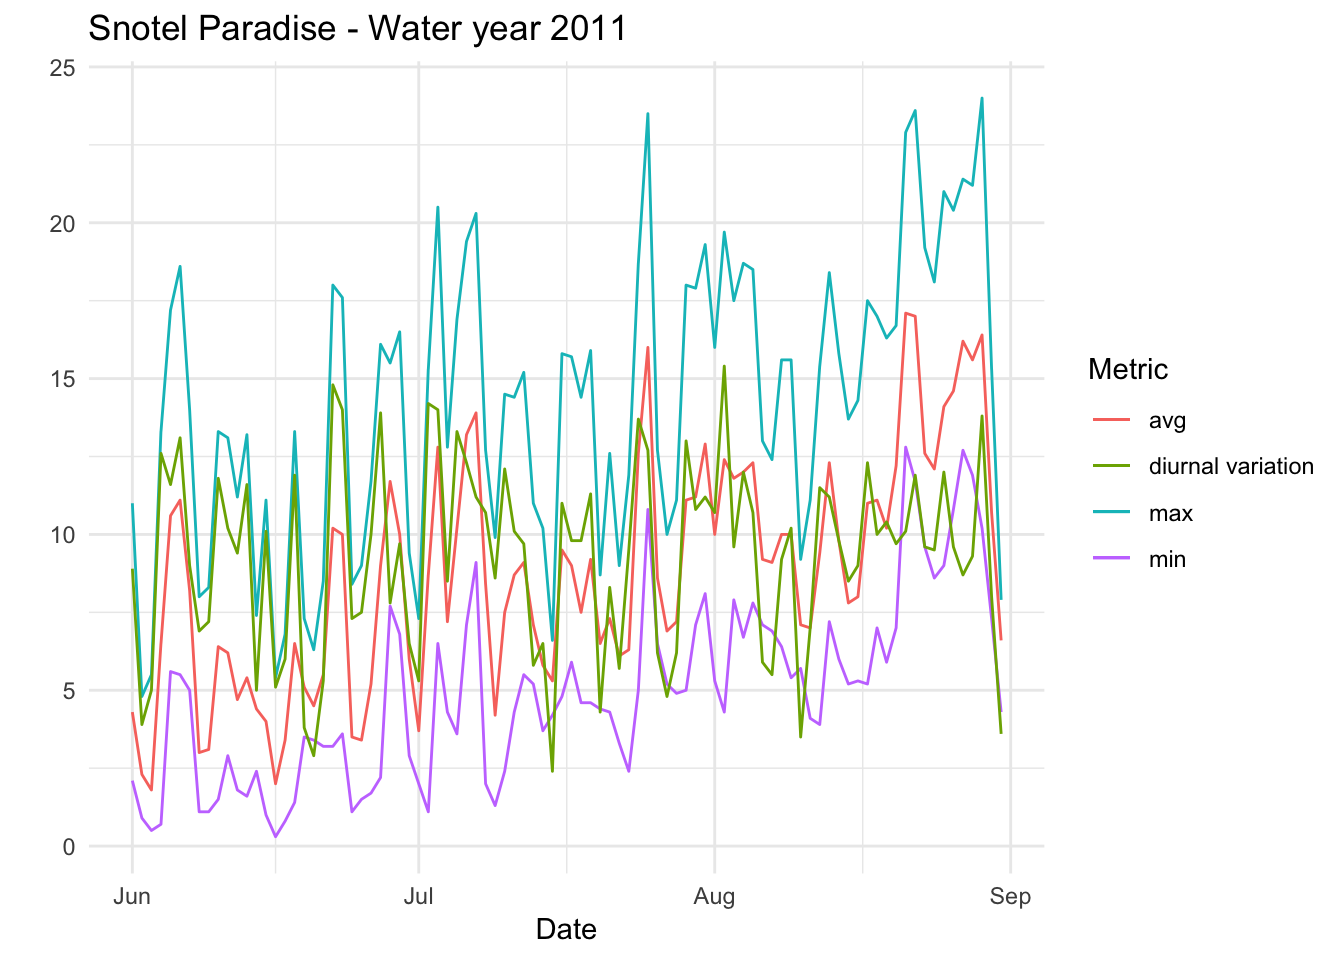
\includegraphics{Research_book_files/figure-latex/unnamed-chunk-31-1.pdf}

\begin{Shaded}
\begin{Highlighting}[]
\CommentTok{#.16}
\end{Highlighting}
\end{Shaded}

\section{7-26-2018}\label{section-7}

Lets look at the diurnal variation for three months, need to switch to
NWAC as Snotel does not provide hourly breakdown

\begin{Shaded}
\begin{Highlighting}[]
\NormalTok{Paradise_5400_}\DecValTok{2017}\NormalTok{<-}\StringTok{ }\KeywordTok{read.csv}\NormalTok{(}\StringTok{'./data/Paradise_5400_feet_2017.csv'}\NormalTok{)}
\NormalTok{Paradise_5400_}\DecValTok{2016}\NormalTok{<-}\StringTok{ }\KeywordTok{read.csv}\NormalTok{(}\StringTok{'./data/Paradise_5400_feet_2016.csv'}\NormalTok{)}
\NormalTok{Paradise_5400_}\DecValTok{2015}\NormalTok{<-}\StringTok{ }\KeywordTok{read.csv}\NormalTok{(}\StringTok{'./data/Paradise_5400_feet_2015.csv'}\NormalTok{)}

\NormalTok{Paradise_5400_}\DecValTok{2017}\OperatorTok{$}\NormalTok{date <-}\StringTok{ }\KeywordTok{as.Date}\NormalTok{(Paradise_5400_}\DecValTok{2017}\OperatorTok{$}\NormalTok{Date.Time..PST., }\StringTok{"%Y-%m-%d"}\NormalTok{)}
\NormalTok{Paradise_5400_}\DecValTok{2017}\OperatorTok{$}\NormalTok{datetime <-}\StringTok{ }\KeywordTok{as.Date}\NormalTok{(Paradise_5400_}\DecValTok{2017}\OperatorTok{$}\NormalTok{Date.Time..PST., }\StringTok{"%Y-%m-%d %H:%M"}\NormalTok{)}
\KeywordTok{library}\NormalTok{(lubridate)}
\KeywordTok{library}\NormalTok{(gridExtra)}
\NormalTok{Paradise_5400_}\DecValTok{2017}\OperatorTok{$}\NormalTok{hr <-lubridate}\OperatorTok{::}\KeywordTok{hour}\NormalTok{(lubridate}\OperatorTok{::}\KeywordTok{as_datetime}\NormalTok{(Paradise_5400_}\DecValTok{2017}\OperatorTok{$}\NormalTok{Date.Time..PST.))}
\NormalTok{Paradise_5400_}\DecValTok{2017}\OperatorTok{$}\NormalTok{min <-lubridate}\OperatorTok{::}\KeywordTok{minute}\NormalTok{(lubridate}\OperatorTok{::}\KeywordTok{as_datetime}\NormalTok{(Paradise_5400_}\DecValTok{2017}\OperatorTok{$}\NormalTok{Date.Time..PST.))}
\NormalTok{Paradise_5400_}\DecValTok{2017}\OperatorTok{$}\NormalTok{month <-}\StringTok{ }\KeywordTok{strftime}\NormalTok{(Paradise_5400_}\DecValTok{2017}\OperatorTok{$}\NormalTok{Date.Time..PST.,}\StringTok{'%m'}\NormalTok{)}
\NormalTok{Paradise_5400_}\DecValTok{2017}\OperatorTok{$}\NormalTok{day <-}\KeywordTok{strftime}\NormalTok{(Paradise_5400_}\DecValTok{2017}\OperatorTok{$}\NormalTok{Date.Time..PST.,}\StringTok{'%d'}\NormalTok{)}

\NormalTok{Paradise9<-}\StringTok{ }\NormalTok{Paradise_5400_}\DecValTok{2017} \OperatorTok\StringTok{ }\KeywordTok{group_by}\NormalTok{(date,month,day,hr) }\OperatorTok\StringTok{ }\KeywordTok{filter}\NormalTok{(}\KeywordTok{as.numeric}\NormalTok{(month) }\OperatorTok\StringTok{ }\KeywordTok{c}\NormalTok{(}\DecValTok{7}\NormalTok{,}\DecValTok{8}\NormalTok{,}\DecValTok{9}\NormalTok{) }\OperatorTok{&}\StringTok{ }\KeywordTok{as.numeric}\NormalTok{(day) }\OperatorTok\StringTok{ }\KeywordTok{c}\NormalTok{(}\DecValTok{9}\NormalTok{) ) }\OperatorTok\StringTok{  }\KeywordTok{ggplot}\NormalTok{() }\OperatorTok{+}\StringTok{  }\KeywordTok{geom_line}\NormalTok{(}\KeywordTok{aes}\NormalTok{(}\KeywordTok{as.numeric}\NormalTok{(hr),Temperature..deg.F.,}\DataTypeTok{group=}\NormalTok{month,}\DataTypeTok{color=}\NormalTok{month)) }\OperatorTok{+}\StringTok{ }\KeywordTok{theme_minimal}\NormalTok{() }\OperatorTok{+}\KeywordTok{xlab}\NormalTok{(}\StringTok{"Hour"}\NormalTok{) }\OperatorTok{+}\StringTok{ }\KeywordTok{ylab}\NormalTok{(}\StringTok{"Temperature"}\NormalTok{) }\OperatorTok{+}\StringTok{ }\KeywordTok{ggtitle}\NormalTok{(}\StringTok{"Paradise 5400 NWAC - Calendar year 2017  - 9th day"}\NormalTok{) }\OperatorTok{+}\StringTok{ }\KeywordTok{scale_color_discrete}\NormalTok{(}\DataTypeTok{name=}\StringTok{"Month"}\NormalTok{)}
\NormalTok{Paradise16<-}\StringTok{ }\NormalTok{Paradise_5400_}\DecValTok{2017} \OperatorTok\StringTok{ }\KeywordTok{group_by}\NormalTok{(date,month,day,hr) }\OperatorTok\StringTok{ }\KeywordTok{filter}\NormalTok{(}\KeywordTok{as.numeric}\NormalTok{(month) }\OperatorTok\StringTok{ }\KeywordTok{c}\NormalTok{(}\DecValTok{7}\NormalTok{,}\DecValTok{8}\NormalTok{,}\DecValTok{9}\NormalTok{) }\OperatorTok{&}\StringTok{ }\KeywordTok{as.numeric}\NormalTok{(day) }\OperatorTok\StringTok{ }\KeywordTok{c}\NormalTok{(}\DecValTok{16}\NormalTok{) ) }\OperatorTok\StringTok{  }\KeywordTok{ggplot}\NormalTok{() }\OperatorTok{+}\StringTok{  }\KeywordTok{geom_line}\NormalTok{(}\KeywordTok{aes}\NormalTok{(}\KeywordTok{as.numeric}\NormalTok{(hr),Temperature..deg.F.,}\DataTypeTok{group=}\NormalTok{month,}\DataTypeTok{color=}\NormalTok{month)) }\OperatorTok{+}\StringTok{ }\KeywordTok{theme_minimal}\NormalTok{() }\OperatorTok{+}\KeywordTok{xlab}\NormalTok{(}\StringTok{"Hour"}\NormalTok{) }\OperatorTok{+}\StringTok{ }\KeywordTok{ylab}\NormalTok{(}\StringTok{"Temperature"}\NormalTok{) }\OperatorTok{+}\StringTok{ }\KeywordTok{ggtitle}\NormalTok{(}\StringTok{"Paradise 5400 NWAC - Calendar year 2017  - 16th day"}\NormalTok{) }\OperatorTok{+}\StringTok{ }\KeywordTok{scale_color_discrete}\NormalTok{(}\DataTypeTok{name=}\StringTok{"Month"}\NormalTok{)}
\NormalTok{Paradise23<-}\StringTok{ }\NormalTok{Paradise_5400_}\DecValTok{2017} \OperatorTok\StringTok{ }\KeywordTok{group_by}\NormalTok{(date,month,day,hr) }\OperatorTok\StringTok{ }\KeywordTok{filter}\NormalTok{(}\KeywordTok{as.numeric}\NormalTok{(month) }\OperatorTok\StringTok{ }\KeywordTok{c}\NormalTok{(}\DecValTok{7}\NormalTok{,}\DecValTok{8}\NormalTok{,}\DecValTok{9}\NormalTok{) }\OperatorTok{&}\StringTok{ }\KeywordTok{as.numeric}\NormalTok{(day) }\OperatorTok\StringTok{ }\KeywordTok{c}\NormalTok{(}\DecValTok{23}\NormalTok{) ) }\OperatorTok\StringTok{  }\KeywordTok{ggplot}\NormalTok{() }\OperatorTok{+}\StringTok{  }\KeywordTok{geom_line}\NormalTok{(}\KeywordTok{aes}\NormalTok{(}\KeywordTok{as.numeric}\NormalTok{(hr),Temperature..deg.F.,}\DataTypeTok{group=}\NormalTok{month,}\DataTypeTok{color=}\NormalTok{month)) }\OperatorTok{+}\StringTok{ }\KeywordTok{theme_minimal}\NormalTok{() }\OperatorTok{+}\KeywordTok{xlab}\NormalTok{(}\StringTok{"Hour"}\NormalTok{) }\OperatorTok{+}\StringTok{ }\KeywordTok{ylab}\NormalTok{(}\StringTok{"Temperature"}\NormalTok{) }\OperatorTok{+}\StringTok{ }\KeywordTok{ggtitle}\NormalTok{(}\StringTok{"Paradise 5400 NWAC - Calendar year 2017  - 23rd day"}\NormalTok{) }\OperatorTok{+}\StringTok{ }\KeywordTok{scale_color_discrete}\NormalTok{(}\DataTypeTok{name=}\StringTok{"Month"}\NormalTok{)}

\KeywordTok{grid.arrange}\NormalTok{(Paradise9,Paradise16,Paradise23)}
\end{Highlighting}
\end{Shaded}

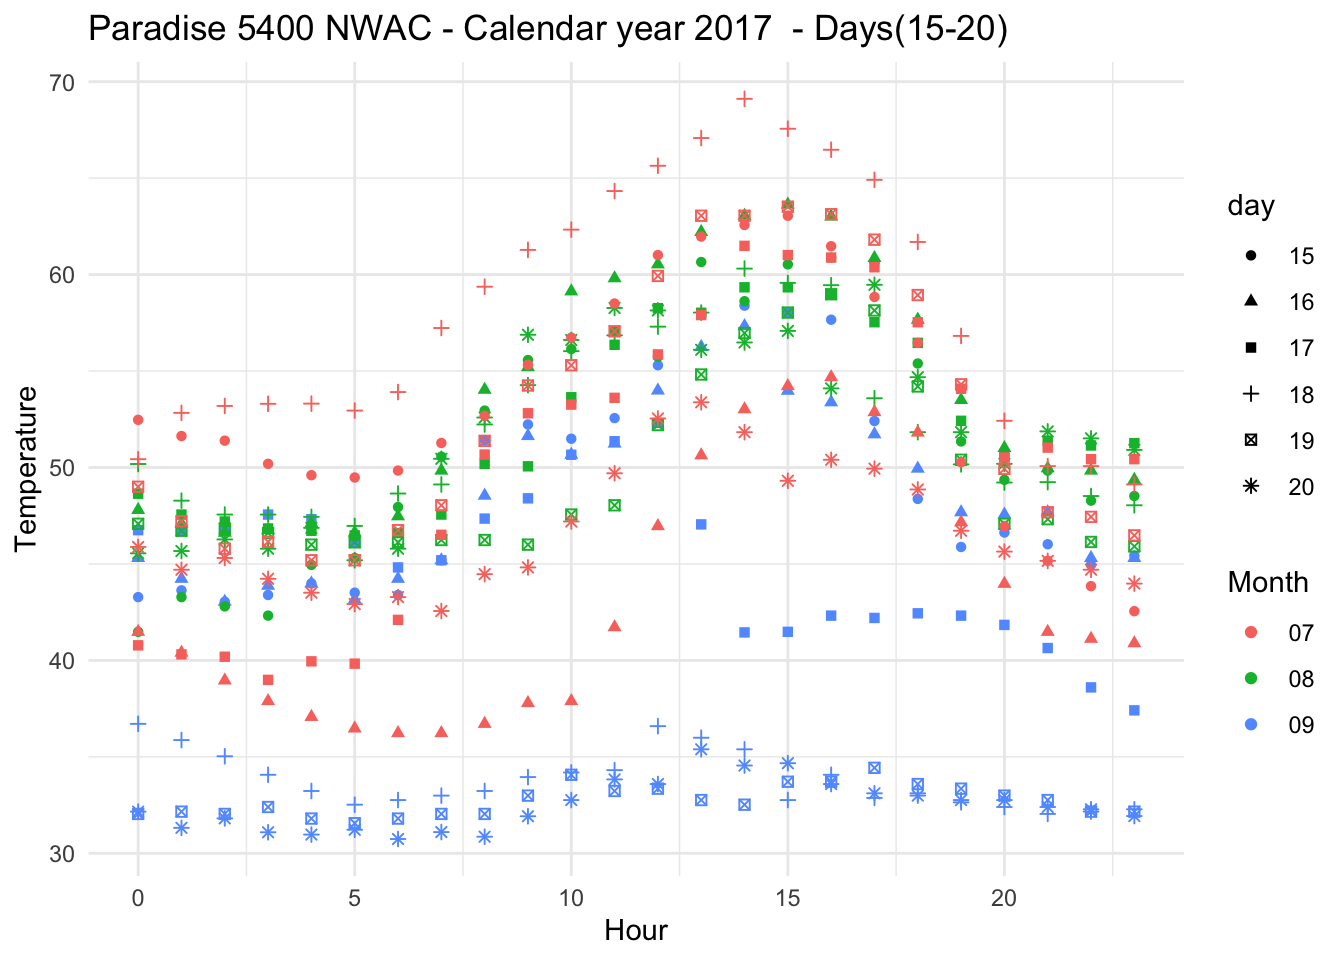
\includegraphics{Research_book_files/figure-latex/unnamed-chunk-32-1.pdf}

Days overlapping eath other

\begin{Shaded}
\begin{Highlighting}[]
\NormalTok{Paradise_5400_}\DecValTok{2017} \OperatorTok\StringTok{ }\KeywordTok{group_by}\NormalTok{(date,month,day,hr) }\OperatorTok\StringTok{ }\KeywordTok{filter}\NormalTok{(}\KeywordTok{as.numeric}\NormalTok{(month) }\OperatorTok\StringTok{ }\KeywordTok{c}\NormalTok{(}\DecValTok{7}\NormalTok{,}\DecValTok{8}\NormalTok{,}\DecValTok{9}\NormalTok{) }\OperatorTok{&}\StringTok{ }\KeywordTok{as.numeric}\NormalTok{(day) }\OperatorTok\StringTok{ }\KeywordTok{c}\NormalTok{(}\DecValTok{15}\NormalTok{,}\DecValTok{16}\NormalTok{,}\DecValTok{17}\NormalTok{,}\DecValTok{18}\NormalTok{,}\DecValTok{19}\NormalTok{,}\DecValTok{20}\NormalTok{) ) }\OperatorTok\StringTok{  }\KeywordTok{ggplot}\NormalTok{() }\OperatorTok{+}\StringTok{  }\KeywordTok{geom_point}\NormalTok{(}\KeywordTok{aes}\NormalTok{(}\KeywordTok{as.numeric}\NormalTok{(hr),Temperature..deg.F.,}\DataTypeTok{shape=}\NormalTok{day,}\DataTypeTok{group=}\DecValTok{7}\NormalTok{,}\DataTypeTok{color=}\NormalTok{month)) }\OperatorTok{+}\StringTok{ }\KeywordTok{theme_minimal}\NormalTok{() }\OperatorTok{+}\KeywordTok{xlab}\NormalTok{(}\StringTok{"Hour"}\NormalTok{) }\OperatorTok{+}\StringTok{ }\KeywordTok{ylab}\NormalTok{(}\StringTok{"Temperature"}\NormalTok{) }\OperatorTok{+}\StringTok{ }\KeywordTok{ggtitle}\NormalTok{(}\StringTok{"Paradise 5400 NWAC - Calendar year 2017  - Days(15-20) "}\NormalTok{) }\OperatorTok{+}\StringTok{ }\KeywordTok{scale_color_discrete}\NormalTok{(}\DataTypeTok{name=}\StringTok{"Month"}\NormalTok{)}
\end{Highlighting}
\end{Shaded}

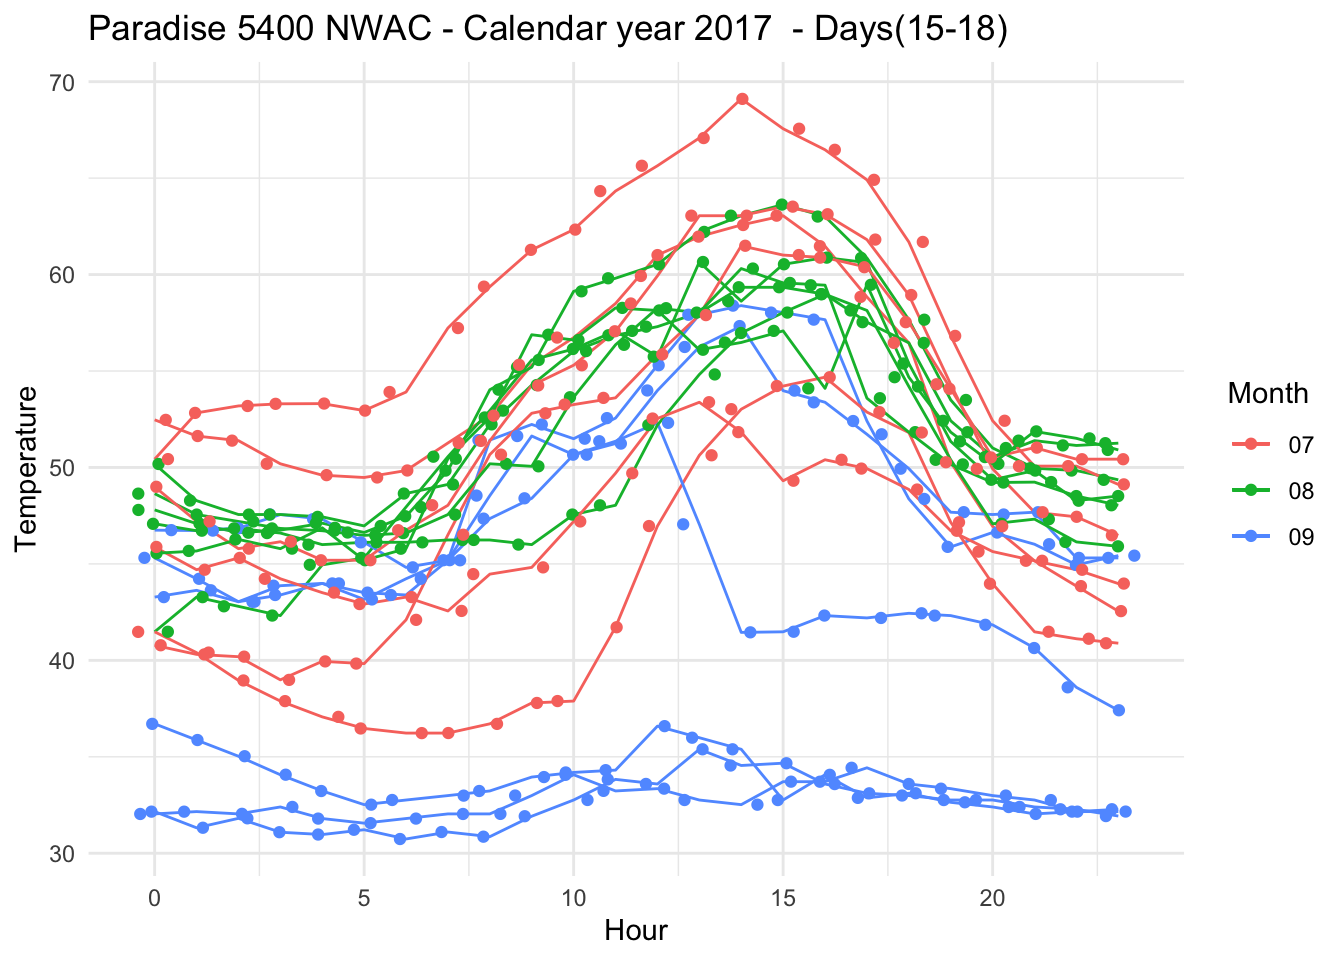
\includegraphics{Research_book_files/figure-latex/unnamed-chunk-33-1.pdf}

Removing symbols, each line representing different day of the month

\begin{Shaded}
\begin{Highlighting}[]
\NormalTok{Paradise_5400_}\DecValTok{2017} \OperatorTok\StringTok{ }\KeywordTok{group_by}\NormalTok{(date,month,day,hr) }\OperatorTok\StringTok{ }\KeywordTok{filter}\NormalTok{(}\KeywordTok{as.numeric}\NormalTok{(month) }\OperatorTok\StringTok{ }\KeywordTok{c}\NormalTok{(}\DecValTok{7}\NormalTok{,}\DecValTok{8}\NormalTok{,}\DecValTok{9}\NormalTok{) }\OperatorTok{&}\StringTok{ }\KeywordTok{as.numeric}\NormalTok{(day) }\OperatorTok\StringTok{ }\KeywordTok{c}\NormalTok{(}\DecValTok{15}\NormalTok{,}\DecValTok{16}\NormalTok{,}\DecValTok{17}\NormalTok{,}\DecValTok{18}\NormalTok{,}\DecValTok{19}\NormalTok{,}\DecValTok{20}\NormalTok{) ) }\OperatorTok\StringTok{ }\KeywordTok{ggplot}\NormalTok{(}\KeywordTok{aes}\NormalTok{(}\DataTypeTok{x =}\NormalTok{ hr, }\DataTypeTok{y =}\NormalTok{ Temperature..deg.F.,}\DataTypeTok{color=}\NormalTok{month)) }\OperatorTok{+}\StringTok{ }\KeywordTok{geom_line}\NormalTok{(}\DataTypeTok{data =} \KeywordTok{subset}\NormalTok{(Paradise_5400_}\DecValTok{2017}\NormalTok{,month }\OperatorTok\StringTok{ }\KeywordTok{c}\NormalTok{(}\StringTok{"07"}\NormalTok{) }\OperatorTok{&}\StringTok{ }\NormalTok{day }\OperatorTok\StringTok{ }\KeywordTok{c}\NormalTok{(}\StringTok{"15"}\NormalTok{)  ))}\OperatorTok{+}\StringTok{ }\KeywordTok{geom_line}\NormalTok{(}\DataTypeTok{data =} \KeywordTok{subset}\NormalTok{(Paradise_5400_}\DecValTok{2017}\NormalTok{,month }\OperatorTok\StringTok{ }\KeywordTok{c}\NormalTok{(}\StringTok{"08"}\NormalTok{) }\OperatorTok{&}\StringTok{ }\NormalTok{day }\OperatorTok\StringTok{ }\KeywordTok{c}\NormalTok{(}\StringTok{"15"}\NormalTok{)  ))}\OperatorTok{+}\StringTok{ }\KeywordTok{geom_line}\NormalTok{(}\DataTypeTok{data =} \KeywordTok{subset}\NormalTok{(Paradise_5400_}\DecValTok{2017}\NormalTok{,month }\OperatorTok\StringTok{ }\KeywordTok{c}\NormalTok{(}\StringTok{"09"}\NormalTok{) }\OperatorTok{&}\StringTok{ }\NormalTok{day }\OperatorTok\StringTok{ }\KeywordTok{c}\NormalTok{(}\StringTok{"15"}\NormalTok{)  ))  }\OperatorTok{+}
\KeywordTok{geom_line}\NormalTok{(}\DataTypeTok{data =} \KeywordTok{subset}\NormalTok{(Paradise_5400_}\DecValTok{2017}\NormalTok{,month }\OperatorTok\StringTok{ }\KeywordTok{c}\NormalTok{(}\StringTok{"07"}\NormalTok{) }\OperatorTok{&}\StringTok{ }\NormalTok{day }\OperatorTok\StringTok{ }\KeywordTok{c}\NormalTok{(}\StringTok{"16"}\NormalTok{)  ))}\OperatorTok{+}\StringTok{ }\KeywordTok{geom_line}\NormalTok{(}\DataTypeTok{data =} \KeywordTok{subset}\NormalTok{(Paradise_5400_}\DecValTok{2017}\NormalTok{,month }\OperatorTok\StringTok{ }\KeywordTok{c}\NormalTok{(}\StringTok{"08"}\NormalTok{) }\OperatorTok{&}\StringTok{ }\NormalTok{day }\OperatorTok\StringTok{ }\KeywordTok{c}\NormalTok{(}\StringTok{"16"}\NormalTok{)  ))}\OperatorTok{+}\StringTok{ }\KeywordTok{geom_line}\NormalTok{(}\DataTypeTok{data =} \KeywordTok{subset}\NormalTok{(Paradise_5400_}\DecValTok{2017}\NormalTok{,month }\OperatorTok\StringTok{ }\KeywordTok{c}\NormalTok{(}\StringTok{"09"}\NormalTok{) }\OperatorTok{&}\StringTok{ }\NormalTok{day }\OperatorTok\StringTok{ }\KeywordTok{c}\NormalTok{(}\StringTok{"16"}\NormalTok{)  ))  }\OperatorTok{+}
\KeywordTok{geom_line}\NormalTok{(}\DataTypeTok{data =} \KeywordTok{subset}\NormalTok{(Paradise_5400_}\DecValTok{2017}\NormalTok{,month }\OperatorTok\StringTok{ }\KeywordTok{c}\NormalTok{(}\StringTok{"07"}\NormalTok{) }\OperatorTok{&}\StringTok{ }\NormalTok{day }\OperatorTok\StringTok{ }\KeywordTok{c}\NormalTok{(}\StringTok{"17"}\NormalTok{)  ))}\OperatorTok{+}\StringTok{ }\KeywordTok{geom_line}\NormalTok{(}\DataTypeTok{data =} \KeywordTok{subset}\NormalTok{(Paradise_5400_}\DecValTok{2017}\NormalTok{,month }\OperatorTok\StringTok{ }\KeywordTok{c}\NormalTok{(}\StringTok{"08"}\NormalTok{) }\OperatorTok{&}\StringTok{ }\NormalTok{day }\OperatorTok\StringTok{ }\KeywordTok{c}\NormalTok{(}\StringTok{"17"}\NormalTok{)  ))}\OperatorTok{+}\StringTok{ }\KeywordTok{geom_line}\NormalTok{(}\DataTypeTok{data =} \KeywordTok{subset}\NormalTok{(Paradise_5400_}\DecValTok{2017}\NormalTok{,month }\OperatorTok\StringTok{ }\KeywordTok{c}\NormalTok{(}\StringTok{"09"}\NormalTok{) }\OperatorTok{&}\StringTok{ }\NormalTok{day }\OperatorTok\StringTok{ }\KeywordTok{c}\NormalTok{(}\StringTok{"17"}\NormalTok{)  ))  }\OperatorTok{+}\StringTok{  }
\KeywordTok{geom_line}\NormalTok{(}\DataTypeTok{data =} \KeywordTok{subset}\NormalTok{(Paradise_5400_}\DecValTok{2017}\NormalTok{,month }\OperatorTok\StringTok{ }\KeywordTok{c}\NormalTok{(}\StringTok{"07"}\NormalTok{) }\OperatorTok{&}\StringTok{ }\NormalTok{day }\OperatorTok\StringTok{ }\KeywordTok{c}\NormalTok{(}\StringTok{"18"}\NormalTok{)  ))}\OperatorTok{+}\StringTok{ }\KeywordTok{geom_line}\NormalTok{(}\DataTypeTok{data =} \KeywordTok{subset}\NormalTok{(Paradise_5400_}\DecValTok{2017}\NormalTok{,month }\OperatorTok\StringTok{ }\KeywordTok{c}\NormalTok{(}\StringTok{"08"}\NormalTok{) }\OperatorTok{&}\StringTok{ }\NormalTok{day }\OperatorTok\StringTok{ }\KeywordTok{c}\NormalTok{(}\StringTok{"18"}\NormalTok{)  ))}\OperatorTok{+}\StringTok{ }\KeywordTok{geom_line}\NormalTok{(}\DataTypeTok{data =} \KeywordTok{subset}\NormalTok{(Paradise_5400_}\DecValTok{2017}\NormalTok{,month }\OperatorTok\StringTok{ }\KeywordTok{c}\NormalTok{(}\StringTok{"09"}\NormalTok{) }\OperatorTok{&}\StringTok{ }\NormalTok{day }\OperatorTok\StringTok{ }\KeywordTok{c}\NormalTok{(}\StringTok{"18"}\NormalTok{)  ))  }\OperatorTok{+}\StringTok{  }
\KeywordTok{geom_line}\NormalTok{(}\DataTypeTok{data =} \KeywordTok{subset}\NormalTok{(Paradise_5400_}\DecValTok{2017}\NormalTok{,month }\OperatorTok\StringTok{ }\KeywordTok{c}\NormalTok{(}\StringTok{"07"}\NormalTok{) }\OperatorTok{&}\StringTok{ }\NormalTok{day }\OperatorTok\StringTok{ }\KeywordTok{c}\NormalTok{(}\StringTok{"19"}\NormalTok{)  ))}\OperatorTok{+}\StringTok{ }\KeywordTok{geom_line}\NormalTok{(}\DataTypeTok{data =} \KeywordTok{subset}\NormalTok{(Paradise_5400_}\DecValTok{2017}\NormalTok{,month }\OperatorTok\StringTok{ }\KeywordTok{c}\NormalTok{(}\StringTok{"08"}\NormalTok{) }\OperatorTok{&}\StringTok{ }\NormalTok{day }\OperatorTok\StringTok{ }\KeywordTok{c}\NormalTok{(}\StringTok{"19"}\NormalTok{)  ))}\OperatorTok{+}\StringTok{ }\KeywordTok{geom_line}\NormalTok{(}\DataTypeTok{data =} \KeywordTok{subset}\NormalTok{(Paradise_5400_}\DecValTok{2017}\NormalTok{,month }\OperatorTok\StringTok{ }\KeywordTok{c}\NormalTok{(}\StringTok{"09"}\NormalTok{) }\OperatorTok{&}\StringTok{ }\NormalTok{day }\OperatorTok\StringTok{ }\KeywordTok{c}\NormalTok{(}\StringTok{"19"}\NormalTok{)  ))  }\OperatorTok{+}\StringTok{ }
\KeywordTok{geom_line}\NormalTok{(}\DataTypeTok{data =} \KeywordTok{subset}\NormalTok{(Paradise_5400_}\DecValTok{2017}\NormalTok{,month }\OperatorTok\StringTok{ }\KeywordTok{c}\NormalTok{(}\StringTok{"07"}\NormalTok{) }\OperatorTok{&}\StringTok{ }\NormalTok{day }\OperatorTok\StringTok{ }\KeywordTok{c}\NormalTok{(}\StringTok{"20"}\NormalTok{)  ))}\OperatorTok{+}\StringTok{ }\KeywordTok{geom_line}\NormalTok{(}\DataTypeTok{data =} \KeywordTok{subset}\NormalTok{(Paradise_5400_}\DecValTok{2017}\NormalTok{,month }\OperatorTok\StringTok{ }\KeywordTok{c}\NormalTok{(}\StringTok{"08"}\NormalTok{) }\OperatorTok{&}\StringTok{ }\NormalTok{day }\OperatorTok\StringTok{ }\KeywordTok{c}\NormalTok{(}\StringTok{"20"}\NormalTok{)  ))}\OperatorTok{+}\StringTok{ }\KeywordTok{geom_line}\NormalTok{(}\DataTypeTok{data =} \KeywordTok{subset}\NormalTok{(Paradise_5400_}\DecValTok{2017}\NormalTok{,month }\OperatorTok\StringTok{ }\KeywordTok{c}\NormalTok{(}\StringTok{"09"}\NormalTok{) }\OperatorTok{&}\StringTok{ }\NormalTok{day }\OperatorTok\StringTok{ }\KeywordTok{c}\NormalTok{(}\StringTok{"20"}\NormalTok{)  ))  }\OperatorTok{+}\StringTok{    }
\KeywordTok{theme_minimal}\NormalTok{() }\OperatorTok{+}\StringTok{ }\KeywordTok{xlab}\NormalTok{(}\StringTok{"Hour"}\NormalTok{) }\OperatorTok{+}\StringTok{ }\KeywordTok{ylab}\NormalTok{(}\StringTok{"Temperature"}\NormalTok{) }\OperatorTok{+}\StringTok{ }\KeywordTok{ggtitle}\NormalTok{(}\StringTok{"Paradise 5400 NWAC - Calendar year 2017  - Days(15-18) "}\NormalTok{) }\OperatorTok{+}\StringTok{ }\KeywordTok{scale_color_discrete}\NormalTok{(}\DataTypeTok{name=}\StringTok{"Month"}\NormalTok{)}\OperatorTok{+}\KeywordTok{geom_jitter}\NormalTok{()}
\end{Highlighting}
\end{Shaded}

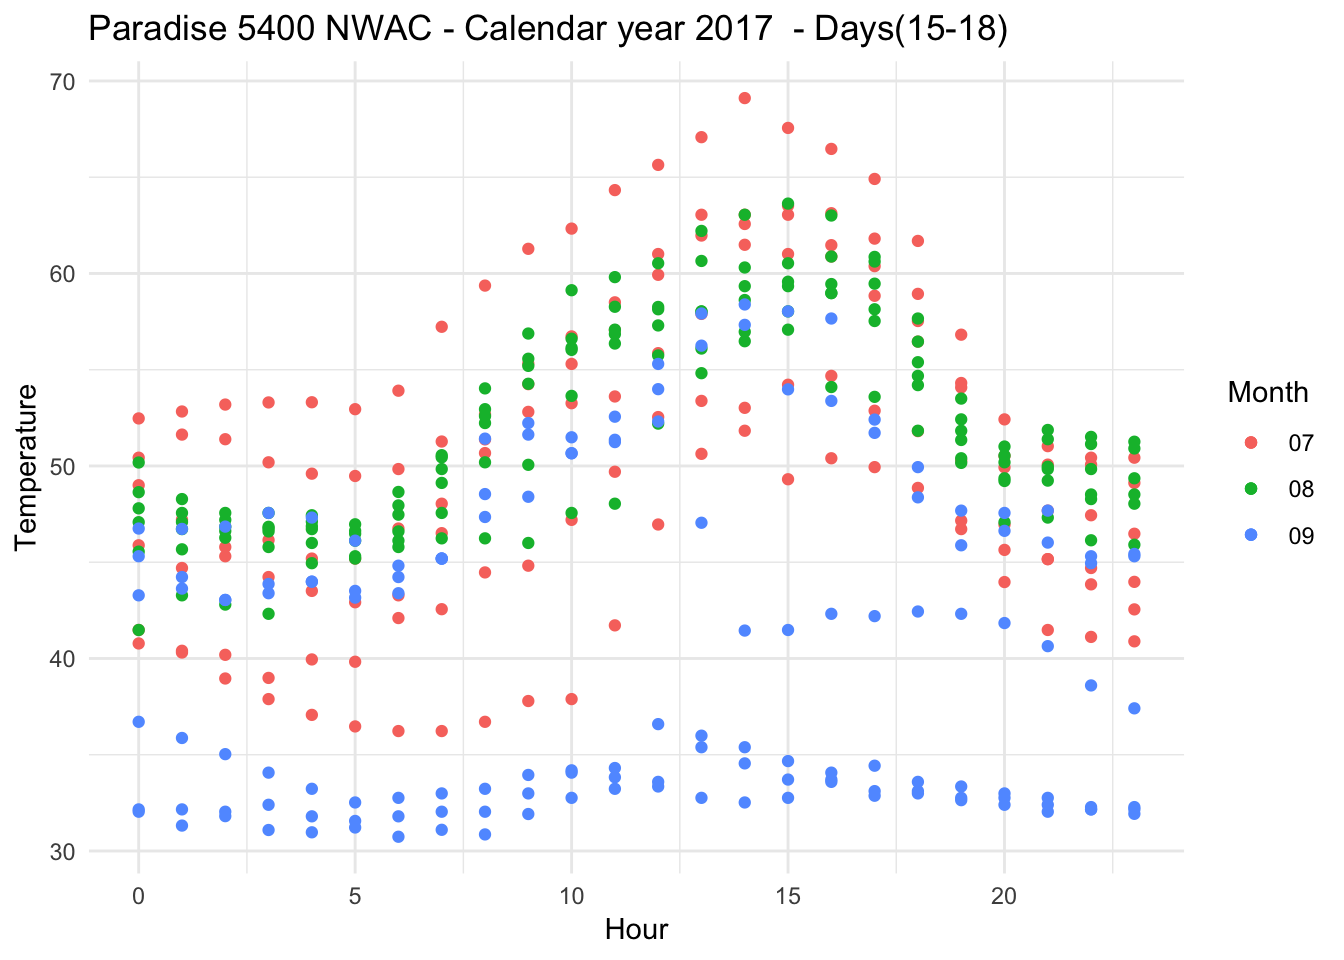
\includegraphics{Research_book_files/figure-latex/unnamed-chunk-34-1.pdf}

Removing symbols, point plot

\begin{Shaded}
\begin{Highlighting}[]
\NormalTok{Paradise_5400_}\DecValTok{2017} \OperatorTok\StringTok{ }\KeywordTok{group_by}\NormalTok{(date,month,day,hr) }\OperatorTok\StringTok{ }\KeywordTok{filter}\NormalTok{(}\KeywordTok{as.numeric}\NormalTok{(month) }\OperatorTok\StringTok{ }\KeywordTok{c}\NormalTok{(}\DecValTok{7}\NormalTok{,}\DecValTok{8}\NormalTok{,}\DecValTok{9}\NormalTok{) }\OperatorTok{&}\StringTok{ }\KeywordTok{as.numeric}\NormalTok{(day) }\OperatorTok\StringTok{ }\KeywordTok{c}\NormalTok{(}\DecValTok{15}\NormalTok{,}\DecValTok{16}\NormalTok{,}\DecValTok{17}\NormalTok{,}\DecValTok{18}\NormalTok{,}\DecValTok{19}\NormalTok{,}\DecValTok{20}\NormalTok{) ) }\OperatorTok\StringTok{ }\KeywordTok{ggplot}\NormalTok{(}\KeywordTok{aes}\NormalTok{(}\DataTypeTok{x =}\NormalTok{ hr, }\DataTypeTok{y =}\NormalTok{ Temperature..deg.F.,}\DataTypeTok{color=}\NormalTok{month)) }\OperatorTok{+}\StringTok{ }\KeywordTok{geom_point}\NormalTok{(}\DataTypeTok{data =} \KeywordTok{subset}\NormalTok{(Paradise_5400_}\DecValTok{2017}\NormalTok{,month }\OperatorTok\StringTok{ }\KeywordTok{c}\NormalTok{(}\StringTok{"07"}\NormalTok{) }\OperatorTok{&}\StringTok{ }\NormalTok{day }\OperatorTok\StringTok{ }\KeywordTok{c}\NormalTok{(}\StringTok{"15"}\NormalTok{,}\StringTok{"16"}\NormalTok{,}\StringTok{"17"}\NormalTok{,}\StringTok{"18"}\NormalTok{,}\StringTok{"19"}\NormalTok{,}\StringTok{"20"}\NormalTok{)))}\OperatorTok{+}\StringTok{ }\KeywordTok{geom_point}\NormalTok{(}\DataTypeTok{data =} \KeywordTok{subset}\NormalTok{(Paradise_5400_}\DecValTok{2017}\NormalTok{,month }\OperatorTok\StringTok{ }\KeywordTok{c}\NormalTok{(}\StringTok{"08"}\NormalTok{) }\OperatorTok{&}\StringTok{ }\NormalTok{day }\OperatorTok\StringTok{ }\KeywordTok{c}\NormalTok{(}\StringTok{"15"}\NormalTok{,}\StringTok{"16"}\NormalTok{,}\StringTok{"17"}\NormalTok{,}\StringTok{"18"}\NormalTok{,}\StringTok{"19"}\NormalTok{,}\StringTok{"20"}\NormalTok{)  ))}\OperatorTok{+}\StringTok{ }\KeywordTok{geom_point}\NormalTok{(}\DataTypeTok{data =} \KeywordTok{subset}\NormalTok{(Paradise_5400_}\DecValTok{2017}\NormalTok{,month }\OperatorTok\StringTok{ }\KeywordTok{c}\NormalTok{(}\StringTok{"09"}\NormalTok{) }\OperatorTok{&}\StringTok{ }\NormalTok{day }\OperatorTok\StringTok{ }\KeywordTok{c}\NormalTok{(}\StringTok{"15"}\NormalTok{,}\StringTok{"16"}\NormalTok{,}\StringTok{"17"}\NormalTok{,}\StringTok{"18"}\NormalTok{,}\StringTok{"19"}\NormalTok{,}\StringTok{"20"}\NormalTok{)  ))  }\OperatorTok{+}\KeywordTok{theme_minimal}\NormalTok{() }\OperatorTok{+}\KeywordTok{xlab}\NormalTok{(}\StringTok{"Hour"}\NormalTok{) }\OperatorTok{+}\StringTok{ }\KeywordTok{ylab}\NormalTok{(}\StringTok{"Temperature"}\NormalTok{) }\OperatorTok{+}\StringTok{ }\KeywordTok{ggtitle}\NormalTok{(}\StringTok{"Paradise 5400 NWAC - Calendar year 2017  - Days(15-18) "}\NormalTok{) }\OperatorTok{+}\StringTok{ }\KeywordTok{scale_color_discrete}\NormalTok{(}\DataTypeTok{name=}\StringTok{"Month"}\NormalTok{)}
\end{Highlighting}
\end{Shaded}

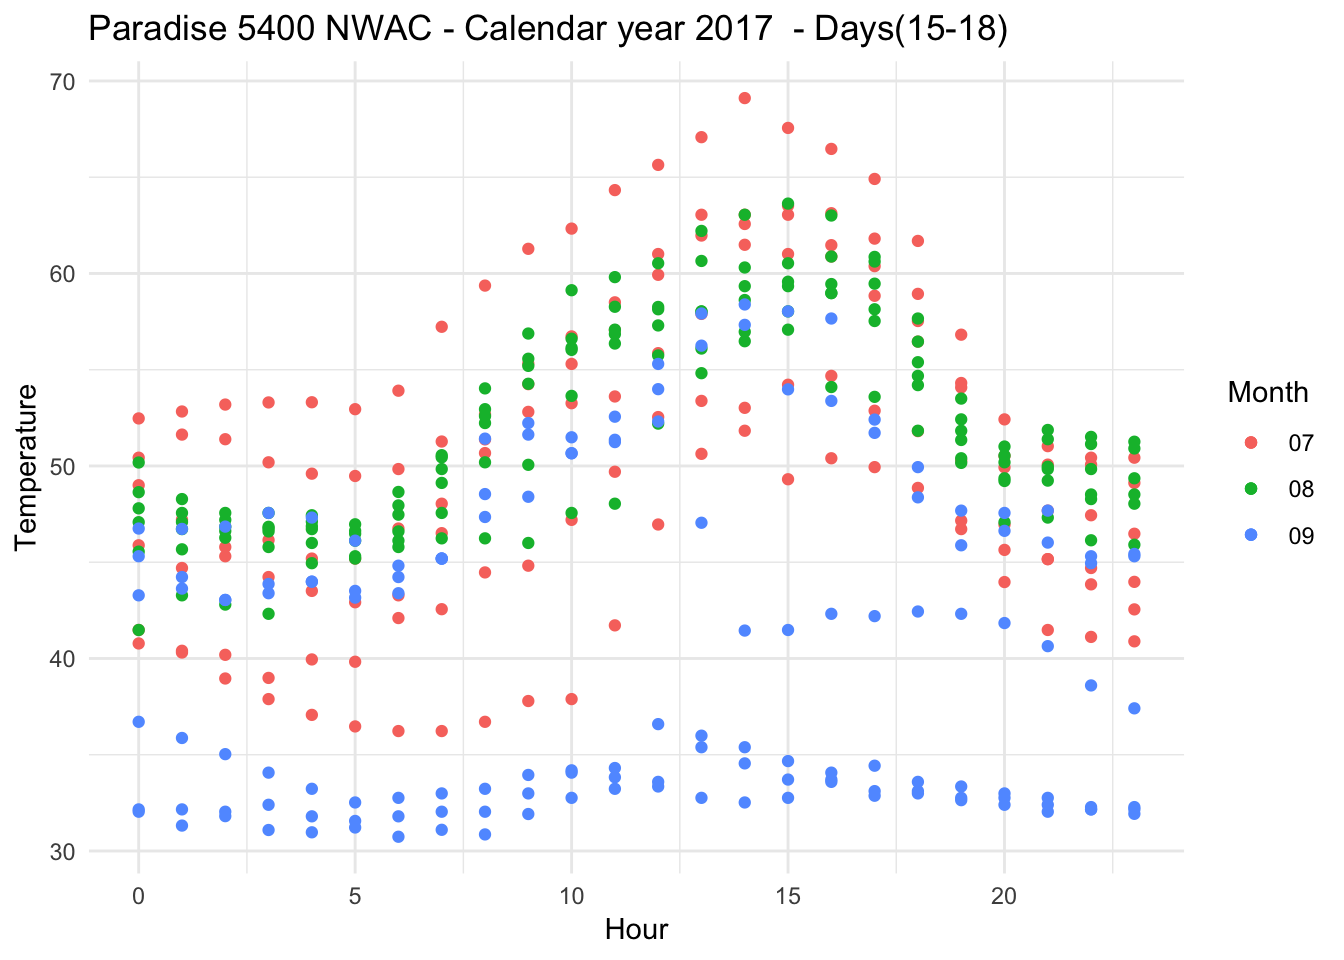
\includegraphics{Research_book_files/figure-latex/unnamed-chunk-35-1.pdf}

\bibliography{book.bib,packages.bib}


\end{document}
